\documentclass[12pt,titlepage,headsepline]{article}
\usepackage[english,ngerman]{babel}
\usepackage[utf8]{inputenc}
\usepackage[a4paper,lmargin={3cm},rmargin={3cm},
tmargin={4cm},bmargin = {3cm}]{geometry}
\usepackage{amsmath}
\usepackage{amssymb}
\usepackage{dsfont}
\usepackage{xcolor}
\usepackage{interval}
\usepackage{ntheorem}
\usepackage{shuffle}
\usepackage{graphicx}
\usepackage{algorithm}
\usepackage{algpseudocode}
\usepackage[style=numeric,sorting=none]{biblatex}
\usepackage[]{listofsymbols}
\usepackage{subfigure}
\usepackage{tabularx}
\usepackage{alphalph}
\renewcommand*{\thesubfigure}{%
\alphalph{\value{subfigure}}%
}%
\usepackage{booktabs}
\usepackage{fancyhdr}

\pagestyle{fancy}
\fancyhf{}
\rhead{\leftmark}

\renewcommand{\baselinestretch}{1.2}
\newtheorem{definition}{Definition}[section]
\newtheorem{theorem}{Theorem}[section]
\newtheorem*{theorem-non}{Theorem}
\newtheorem{corollary}[theorem]{Korollar}
\newtheorem*{corollary-non}{Korollar}
\newtheorem{lemma}[theorem]{Lemma}
\newtheorem*{lemma-non}{Lemma}
\newtheorem*{beweis}{Beweis}
\newtheorem*{beweis-non}{Beweis}
\newtheorem{beispiel}[definition]{Beispiel}
\newtheorem*{beispiel-non}{Beispiel}
\newtheorem*{bemerkung*}{Bemerkung}

\graphicspath{ {../pics/} }
\addbibresource{masterarbeit.bib}



\begin{document}

    \begin{titlepage}
      \begin{center}
        %\vspace*{1cm}
        
\includegraphics[width=0.3\textwidth]{TU.png}\\
        Technische Universität Berlin \\
        Fakultät II - Mathematik und Naturwissenschaften\\
        Institut für Mathematik

        \vspace{1.5cm}
        \LARGE
        \textbf{Optimales Stoppen mit der Signaturmethode}

        \vspace{1.5cm}
        \Huge
        \textbf{Masterarbeit}

        \vspace{1cm}
        \small
        \text{vorgelegt von}

        \large
        \textbf{Zhongdi Xu}

        \vspace{4cm}

        \small{\scshape
        \begin{tabular}{rl}
         Matrikelnummer: & 357376 \\
         Studiengang: & Mathematik M.Sc.\\
         Erstgutachter: & Dr. habil. Sebastian Riedel\\
         Zweitgutachter: & Prof. Dr. Peter Friz \\
         Abgabe am: & 30.09.2021\\
         \end{tabular}
        }

      \end{center}
    \end{titlepage}
    \newpage
    \tableofcontents
    \newpage

    \section*{Eidesstattliche Erklärung}
    \thispagestyle{empty}
    Hiermit erkläre ich, dass ich die vorliegende Arbeit selbstständig und eigenhändig sowie ohne unerlaubte fremde Hilfe und ausschließlich unter Verwendung der aufgeführten Quellen und Hilfsmittel angefertigt habe.

    \vspace{0.5cm}
    \hfill\break
    Berlin, den

    \vspace{1cm}
    \hfill\break
    $\ldots\ldots\ldots\ldots\ldots\ldots\ldots\ldots\ldots\ldots\ldots\ldots\ldots\ldots$
    \hfill\break
    Unterschrift
    \newpage

    \section*{Dankesagung}
    \thispagestyle{empty}
    An dieser Stelle möchte ich mich bei all denjenigen bedanken, die mich während der Anfertigung dieser Masterarbeit unterstützt und motiviert haben.
    \hfill\break
    Zuerst gebührt mein Dank Herr Dr. Sebastian Riedel und Prof. Dr. Jochen Diehl, die meine Masterarbeit betreut und begutachtet haben. Für die hilfreichen Anregungen und die konstruktive Kritik bei der Erstellung dieser Arbeit möchte ich mich herzlich bedanken.
    \hfill\break
    Ebenfalls möchte ich mich bei meinem Vorgesetzten Dr. Dmitri Topaj bedanken, der mir mit viel Geduld, Interesse und Hilfsbereitschaft zur Seite stand.
    \hfill\break
    % Außerdem möchte ich Anna Fried für das Korrekturlesen meiner Masterarbeit danken.
    % \hfill\break
    Abschließend möchte ich mich bei meiner Frau Qi Gao und meinen Eltern bedanken, die mir mein Studium durch ihre Unterstützung ermöglicht haben und stets ein offenes Ohr für mich hatten.

    \newpage

    \begin{otherlanguage}{english}
      \begin{abstract}
        In dieser Arbeit untersuchen wir zwei neue Methoden für das optimale Stoppen, die \textit{Signaturmethode} und \textit{Hybridmethode}. Beide Methoden sind durch die Signatur vom Rough Path inspiriert worden, womit man die Signatur Stoppzeit hergeleitet hat. Im Vergleich zu den konventionellen Ergebnissen für das optimale Stoppen benötigen wir von dem Prozess weder die Martingaleigenschaft noch, dass der Prozess markovisch ist. Die einzige Voraussetzung ist es, dass der Prozess ein geometrische Rough Path ist. Für die numerische Untersuchung verwenden wir die fraktionale Brownsche Bewegung als das Testobjekt und die Resultate aus \cite{becker_deep_2019} als Benchmark. Die numerische Ergebnisse zeigen, dass die Signaturmethode zwar in der Berechnung deutlich schneller ist, jedoch eine geringe Präzision als die Hybridmethode aufweist.
      \end{abstract}
    \end{otherlanguage}
    \newpage

    \begin{otherlanguage}{english}
      \begin{abstract}
        In this thesis we investigate two new methods for optimal stopping problem, the \textit{signature method} and \textit{hybrid method}. Both methods were inspired by the signature from the Rough Path, which was used to derive the signature stopping time. Compared to the conventional results for optimal stopping problem, we neither need the martingale property of the process nor that the process is Markovian. The only requirement is that the process be a geometric rough path. For the numerical investigation we use the fractional Brownian motion as the test object and the results from \cite{becker_deep_2019} as the benchmark. The numerical results show that the signature method is significantly faster in the calculation, but has a lower precision than the hybrid method.
      \end{abstract}
    \end{otherlanguage}
    \newpage

    \pagestyle{fancy}
    \fancyhf{}
    \rhead{\leftmark}
    \lhead{Zhongdi Xu}
    \cfoot{\thepage}

    \section{Einleitung}
    Das optimale Stoppen \cite{peskir_optimal_2006} für Zufallsprozesse hat seine Wichtigkeit in der Physik, dem Ingenieurwesen und in der Finanzmathematik. Dabei sei $(\Omega,\mathcal{F},(\mathcal{F}_t)_{t\geq 0},\mathbb{P})$ ein gefilterter Wahrscheinlichkeitsraum und $X=(X_t)_{t\geq 0}$ ein adaptierter stochastischer Prozess bezüglich der Filtration $(\mathcal{F}_t)_{t\geq 0}$. Ein Prozess $X_t$ heißt adaptiert, wenn $X_t$ $\mathcal{F}_t$-messbar für alle $t \geq 0 $ ist. Die Klasse aller Stoppzeiten $\tau$ auf dieser Filtration ist gegeben durch
    $\mathcal{T}_T$ mit $T \in [0,T]$. Wir wissen aus der Stochastik, dass die Stoppzeiten Zufallsvariablen sind mit den Eigenschaften
    $0 \leq \tau \leq T$, $\tau(\omega)< \infty$ fast sicher und $\{\omega : \tau(\omega) \leq t\} \in \mathcal{F}_t$ für alle $t\geq 0$.
    \hfill\break
    Für das optimale Stoppen suchen wir nach dem maximalen Erwartungswert von $X$:
    \begin{align*}
      V = \underset{\tau \in \mathcal{T}_T}{max} \ \mathbb{E}[X_{\tau}]
    \end{align*}
    und die Stoppzeit $\tau^* \in \mathcal{T}_T$, in der das Supremum erreicht wird, falls diese existiert.
    \hfill\break
    %Für adaptierter Prozess $X_t$ nennen wir das optimale Stoppen für $V$ das \textit{Standardproblem} und andernfalls nennen wir es das \textit{Nicht-Standardproblem}. Die allgemeinte optimales Stoppen Theorie ist für Standardprobleme gut erforscht, so dass man bei den Nicht-Standardproblemen diese auf die Standardprobleme zurückführen, um sie zu lösen.
    \hfill\break
    Für das Lösen des optimale Stoppens gibt es zwei klassische Ansätze aus der Stochastik: der Martingalansatz und der Markovsche Ansatz. In dem Martingalansatz löst man das optimale Stoppen mit zwei Methoden, die Rückwärtsinduktion und das Essentielle Supremum. Die Methode der Rückwärtsinduktion funktioniert im diskreten Fall wie folgt: sei $(\Omega,\mathcal{F},(\mathcal{F}_n)_{n \leq N},\mathbb{P})$ ein gefilterter Wahrscheinlichkeitsraum mit $\mathcal{F}_0 \subseteq \mathcal{F}_1 \subseteq \ldots \subseteq \mathcal{F}_N \subseteq \mathcal{F}$ und eine Zufallsfolge $X_0,X_1,\ldots,X_N$ mit:
    \begin{align*}
      \mathbb{E}[X_n] < \infty \quad \textup{für alle} \quad n=1,\ldots,N.
    \end{align*}
    Das Problem $V = \underset{\tau \in \mathcal{T}_N}{max} \ \mathbb{E}[X_{\tau}]$ mit der Klasse der ganzzahligen Stoppzeiten lösen wir mit der Rückwärtsinduktion, indem wir eine zusätzliche Zufallsfolge $W_1,\ldots,W_N$ rückwärts konstruieren:
    \begin{align*}
      W_N &= X_N \\
      W_n &= max(X_n,\mathbb{E}[X_{n+1} \lvert \mathcal{F}_n]),
    \end{align*}
    welche den maximalen möglichen Wert im Zeitpunkt $n$ reflektiert. Für $n=N$ stoppen wir sofort und erhalten den Wert $W_N = X_N$. Für $n<N$ können wir die Wahl treffen, zu stoppen oder fortzusetzen. Wenn wir stoppen, dann ist der Wert $X_n$ und wenn wir weitergehen, ist der Wert $\mathbb{E}[X_{n+1} \lvert \mathcal{F}_n]$. Darauf basierend betrachten wir für die optimale Stoppzeit den folgenden Kandidaten:
    \begin{align*}
      \tau^* = inf\{k \leq N : W_k = X_k \},
    \end{align*}
    d.h. wir stoppen an dem Zeitpunkt, wo der maximale mögliche Wert den Wert von $X$ zu dem Zeitpunkt nicht überschreitet. Für die so definierte Stoppzeit hat man bewiesen, dass diese eine optimale Stoppzeit und sogar die kleinste optimale Stoppzeit ist. Für den Prozess $(W_n)_{n\leq N}$ hat man die Supermartingaleigenschaft gezeigt. Zusätzlich ist $(W_n)_{n\leq N}$ das kleinste Supermartingal, welches den Prozess $(X_n)_{n\leq N}$ dominiert. Man hat auch gezeigt, dass $(W_{n \wedge \tau^*})_{n\leq N}$ ein Martingal ist.
    \hfill\break
    Die Methode des essentiellen Supremums erweitert die Rückwärtsinduktion. Dabei betrachten wir das Problem in der stetigen Zeit:
    \begin{align*}
      V_t^T = \underset{t\leq \tau \leq T}{sup} \mathbb{E}[X_{\tau}].
    \end{align*}
    Wir lösen es mithilfe einer Snell-Envelope $(W_t)\_{t\geq 0}$ von dem Prozess $X$. Für die Konstruktion fordern wir zwei Bedingung an $X$: 1. $(X_t)_{t \geq 0}$ soll ein rechtsstetiger Prozess mit linksseitigem Grenzwert. 2. $\mathbb{E}[\underset{0\leq t \leq T}{sup} \lvert X_t \rvert] < \infty$ sein. Dann ist die Snell-Envelope als das kleinste rechtsstetige Supermartingal konstruiert, welches $X$ dominiert:
    \begin{align*}
      W_t = \underset{\tau \geq t}{ess \ sup} \mathbb{E}[G_{\tau} \lvert \mathcal{F}_t].
    \end{align*}
    Dazu definieren wir die Markov-Zeit $\tau^*_t = inf\{u \geq t : W_u = X_u \}$ mit $inf \varnothing = \infty$. Man hat bewiesen, dass die so definierte Markov-Zeit eine optimale Stoppzeit für $V_t$ ist und zwar die kleinste. Mit $(W_{u\wedge \tau^*_t})_{u\geq t}$ erhalten wir ein rechtsstetiges Martingal.

    \hfill\break
    In dem markovschen Ansatz geht man davon aus, dass der Prozess $X_t$ eine markovsche Repräsentation besitzt, d.h. es existiert einen stark markovschen Prozess $Y_t$, so dass
    \begin{align*}
      X_t(\omega) = g(t,Y_t(\omega))
    \end{align*}
    mit einer messbarer Funktion $g(t,x)$ für alle $t\geq 0 $ fast sicher gilt.
    Wir betrachten hier den Wahrscheinlichkeitsraum $(\Omega,\mathcal{F},\mathbb{P}_x)$, wobei hier $x \in \mathbb{R}^d$, $\mathbb{P}_x (X_0 = x)=1$ und $x \mapsto \mathbb{P}_x(A)$ messbar für alle $A \in \mathcal{F}$. Das optimale Stoppen schreiben wir um:
    \begin{align*}
      V(x) = \underset{\tau \in \mathcal{T}}{sup} \mathbb{E}_x[g(X_{\tau})],
    \end{align*}
    wobei $\mathcal{T}$ die Klasse der $\mathbb{P}_x$ fast sicher endlichen Stoppzeiten auf der von $X$ erzeugten Filtration $\mathcal{F}_t^X=\sigma(X_s : s \leq t)$ ist und $g$ die Gain-Funktion. Wir führen zwei Mengen ein: die Menge für die Fortsetzung $F = \{x\in \mathbb{R}^d : V(x) > g(x) \}$ und die Menge für das Stoppen $S= \{x\in \mathbb{R}^d : V(x) = g(x) \}$. Als den Kandidaten für die optimale Stoppzeit betrachten wir $\tau_S = inf \{t \geq 0 : X_t \in S\}$.

    \hfill\break
    In unserer Arbeit verwenden den Signatur Ansatz aus der Rough Path Theorie. Dabei setzen wir nur voraus, dass der zugrundeliegende stochastische Prozess ein \textit{geometrsicher Rough Path} ist. Dies beinhaltet sowohl die Martingale und die markovsche Prozesse als auch die nicht-markovsche Prozesse. Die Idee von \cite{bayer_optimal_2020} ist es, dass man die Signatur Stoppzeit für das optimale Stoppen anwendet. Wir werden sehen, dass das Ersetzen der \textit{normalen} Stoppzeit durch die Signatur Stoppzeit den Wert vom Erwartungswert des betrachteten Prozesses nicht verändert. Wir betrachten die Eintrittszeiten als Stoppzeiten in dieser Arbeit.
    \hfill\break
    In der numerische Implementierung untersuchen wir zwei neue Methoden für das optimale Stoppen für nicht markovsche Prozesse. Die Kernidee beider Methoden ist die Verwendung der Signatur Stoppzeit. Aus dem Resultat von \cite{bayer_optimal_2020}:
    \begin{align}\label{eqn: bayer_result}
      \underset{l \in T((\mathbb{R}^{1+d})^*)}{sup} \ \mathbb{E}[Y_{\tau_l \land T}] = \underset{\tau \in \mathcal{S}}{sup} \ \mathbb{E}[Y_{\tau \land T}]
    \end{align}
    mit $\tau_l := inf \ \bigg\{ t \in [0,T] : \langle l,\hat{\mathbb{X}}^{<\infty}_{0,t}\rangle \geq 1 \bigg\}$ hat man die Gleichheit zwischen dem maximalen Erwartungswert, bestimmt durch die Signatur Stoppzeit, und dem theoretisch maximalen Erwartungswert.
    \hfill\break
    Damit man das Polynom $l \in T((\mathbb{R})^*)$ für die Definition der Klasse für die Stoppzeiten von Rough Paths verwenden kann, führte man die Signatur Stopp Police und die randomisierten Signatur Stoppzeiten ein. Es wurde gezeigt, dass die Gleichung (\ref{eqn: bayer_result}) auch mit der Klasse der randomisierten Stoppzeiten gilt.
    \hfill\break
    Beider Methoden unterscheiden sich in der Bestimmung des Polynoms $l$. In der Signaturmethode generieren wir zufällige Stichproben für den getesteten Prozess, berechnen für jede Stichprobe die Signatur mit einem festen Niveau $N$ und lösen das lineare Gleichungssystem $\langle l,\hat{\mathbb{X}}^{\leq N}_{0,t}\rangle = 1$. In der Hybridmethode orientieren wir uns an \cite{becker_deep_2019}, indem wir die Stoppzeit mithilfe von optimalen Stoppentscheidungen $f_n^l := \mathds{1}_{ \{ \langle l, \hat{\mathbb{X}}^{\leq N}_{0,t_n}  \rangle \geq 1 \} }$ in den einzelnen Schritten $t_n$ zerlegen, die jeweils durch die Maximierung des Funktionals:
    \begin{align*}
      l_n^* = \underset{l \in \mathcal{T}((\mathbb{R}^{1+d})^*)}{argmax} \ \mathbb{E}[g(t_n, Y_{t_n})F_n^l(\hat{\mathbb{X}}^{\leq N})+g(\tau_{n+1},Y_{\tau_{n+1}})(1-F_n^l(\hat{\mathbb{X}}^{\leq N})) ]
    \end{align*}
    mit Monte Carlo Approximation bestimmt sind. $F_n^l(\hat{\mathbb{X}}^{\leq N}) = \psi( \langle l, \hat{\mathbb{X}}^{\leq N}_{0,t_n} \rangle - 1)$ ist die Approximation für $f_n^l$ mit der logistischer Funktion $\psi$, damit wir die gradientenbasierte Optimierungsmethoden verwenden können. Die optimale Stoppzeit ist gegeben durch
    \begin{align*}
      \tau^* := \sum_{n=1}^K t_nf_n^{l_n}(\hat{\mathbb{X}}^{\leq N})\prod_{j=0}^{n-1}(1-f_j^{l_j}(\hat{\mathbb{X}}^{\leq N}))
    \end{align*}
    \hfill\break
    Wir teilen die gleiche theoretische Resultate wie in \cite{bayer_optimal_2020}. In der Arbeit hat man das optimale Stoppen mit Rough Path zunächst die Gleichung (\ref{eqn: bayer_result}) linearisiert:
    \begin{align}\label{eqn: bayer_linearisation}
       \underset{\tau \in \mathcal{S}}{sup} \ \mathbb{E}[Y_{\tau \land T}] &= \underset{l \in T((\mathbb{R}^{1+d})^*)}{sup} \ \mathbb{E}[Y_{\tau_l \land T}] \\
       &= \underset{l \in T((\mathbb{R}^{1+d})^*)}{sup} \ \mathbb{E}[\int_0^T exp(-\int_0^t \langle l,\hat{\mathbb{X}}^{<\infty}_{0,t}\rangle ^2 ds) dY_t] + \mathbb{E}[Y_0].
    \end{align}
    Um das Problem in dieser Form lösen zu können, linearisiert man $exp(-\int_0^t \langle l,\hat{\mathbb{X}}^{<\infty}_{0,t}\rangle ^2 ds)$. Dazu führte man das \textit{Expoential Shuffle} ein. Das Expoential Shuffle definiert man als $exp^{\shuffle}(l):=exp(a_0)exp^{\shuffle}(\tilde{l})$, wobei $a_0\varnothing + \tilde{l} = l \in T(V^*)$ mit
    $\langle \tilde{l}, \mathds{1} \rangle = 0$ und $exp^{\shuffle}(\tilde{l}) = \sum_{r=0}^{\infty}\frac{1}{r!}\tilde{l}^{\shuffle r}$ ist. Damit lässt sich die rechte Seite der Gleichung (\ref{eqn: bayer_linearisation}) durch das Expoential Shuffle beschreiben und mit der Stoppzeit
    $S = S_{\kappa}=inf\{t \geq 0 : \lVert \hat{\mathbb{X}} \rVert_{p-var;[0,t]} \geq \kappa\}\wedge T$
    erreicht man die Konvergenz gegen den optimalen Wert \cite{bayer_optimal_2020,Prop.6.5}:
    \begin{align*}
      \underset{\tau \in \mathcal{S}}{sup} \ \mathbb{E}[Y_{\tau \land T}] = \underset{\kappa \rightarrow \infty}{lim} \underset{K \rightarrow \infty}{lim} \underset{N \rightarrow \infty}{lim} \underset{\lvert l \rvert + deg(l) \leq K)}{sup} \ \mathbb{E}[\int_0^{S_{\kappa}} \langle exp^{\shuffle}(-(l \shuffle l)\textcolor{blue}{1},\hat{\mathbb{X}}^{\leq N}_{0,t}\rangle dY_t] + \mathbb{E}[Y_0].
    \end{align*}
    \hfill\break
    Im Kapitel 2 unserer Arbeit wird die Kurzfassung für die Rough Path Theorie vorgestellt, die für das Grundverständnis dieser Arbeit dient. Für interessierte Leser sind die entsprechenden Stellen an vertiefende Literaturen verwiesen. Wir führen zunächst die Tensoralgebra und die notwendigen Operationen für das Polynom $l$ ein, denn die Signaturen sind Elemente aus der Tensoralgebra. Wir stellen auch vor, dass es zwischen der Basis von der Tensoralgebra $T(V^*)$ und dem Raum der Wörter einen Isomorphismus exisiert, welchen die Einführung von dem Polynom motiviert. Im Anschluss präsentieren wir den p-geometrischen Rough Path als den p-schwach geometrischen Rough Path in der abgeschlossenen Menge, worin die durch $\lfloor p \rfloor$ abgeschnittenen Signaturen von den stückweise glatten Pfaden liegen. Danach kommt das optimale Stoppen mit Rough Path, wo wir das Konzept und die wichtige Theoreme und Resultate aus \cite{bayer_optimal_2020} erläutern. Insbesondere gehen wir auf die Herleitung der Signatur Stoppzeit ein.
    Im Kapitel 3 erläutern wir die Kernidee von \cite{becker_deep_2019}, welche uns die Entwicklung der Hybridmethode motiviert hat. Dabei erläutern wir die Struktur der Stoppzeit, das Konzept mit der Stoppentscheidung sowie die Konvergenzanalyse für das tiefneuronale Netzwerk. Die Konzepte unserer beiden Methoden werden hier präsentiert und die Beschreibung für die numerische Implementierung werden ebenfalls erläutert.
    Im Kapitel 4 diskutieren wir die numerische Resultate und den Vergleich zu \cite{bayer_optimal_2020} und \cite{becker_deep_2019}. Dabei nehmen wir das Resultat für die fraktionale Brownsche Bewegung aus \cite{becker_deep_2019} als Benchmark und verwenden das Konzept für die numerische Implementierung, welches die Relation zwischen dem Hurst Parameter $H$ und dem Erwartungswert $\mathbb{E}[Y_{\tau^*}]$ darstellt. Zusätzlich gehen wir auf die Rechenzeit mit verschiedenen Datengrößen ein. Wir werden sehen, dass die Signaturmethode deutlich schneller ist, aber auch eine deutlich schlechtere Qualität als die Hybridmethode hat.
    Abschließend geben wir dem Leser einen Ausblick über die weitere Forschungsmöglichkeiten zu Optimalem Stoppen mit der Signaturmethode.
    \newpage

    \section{Das optimale Stoppen mit Rough Path}\label{chapter: opt_stop_with_rough_path}

      \subsection{Motivation}
      In der Theorie für die stochastischen Differentialgleichungen (SDE) versucht man die Gleichung der Form $dY_t = \alpha(Y_t)dX_t$ mit einem gegebenen Anfangswert $Y_0 = y$ oder einem Endwert $Y_T = y$ mit $y\in \mathbb{R}^d$ zu lösen, wobei $X, Y$ Zufallsprozesse mit Werten in $\mathbb{R}^d$ sind. Eine Möglichkeit für das Lösen solcher SDE ist die Darstellung in die Integralform:
      \begin{align}\label{integral_gleichung}
        Y_t = Y_0 + \int_0^t \alpha(Y_t)dX_t.
      \end{align}
      Doch jede Realisierung von $Y_t$ bzw. $X_t$ ist ein Prozess von unendlichen Variationen z.B. die Brownsche Bewegung. Wir kennen aus der stochastischen Analysis, dass die Integrationstheorie von Lebesque-Stieltjes darauf nicht anwendbar ist. Ein Ausweg dafür ist die Itô's Integrationstheorie. Wir fordern zusätzliche Eigenschaften wie die Martingaleigenschaft von $X$ und die Vorhersehbarkeit von $Y$ und bilden das Integral über das Martingal. Das Integral selbst ist dann wieder ein Martingal. Damit kann man die SDE der Form (\ref{integral_gleichung}) lösen und das liefert die moderne Mathematik viele Anwednungsmöglichkeiten in Physik, Engenieurwesen, Biologie und Finanzmathematik. Diese Theorie lässt sich auf die Klasse der Semimartingale erweitern, in dem man einen Prozess von endlichen Variationen zu dem Martingal addiert, d.h. ein Semimartingal $W$ definieren wir mit $W_t = W_0 + M_t + A_t$, wobei $M_t$ ein Martingal ist und $A_t$ ein Prozess von endlichen Variationen mit $M_0 = 0 = A_0$ ist. Eine solche Zerlegung nennt man \textit{Doob-Meyer-Zerlegung}.
      \hfill\break
      In \cite{friz_multidimensional_2009} hat man auch für interessante Prozessen wie die fraktionale Brownsche Bewegung (FBM) gezeigt, dass man für $H > 1/2$ ein nicht-markovsches System oder einen arbitragefreien Markt unter Rücksicht der Transaktionskosten modellieren kann. Man kann H so anpassen, dass der stochastischer Prozess gleichgradig nah zu einer Brownsche Bewegung ist. Damit kann man diesen Fall auch lösen. Doch was passiert mit den anderen Fällen wie $H < 1/2$ oder auch $H > 2/3$ ?
      % Erläuterung des Konzepts von Rough Path
      \hfill\break
      Lyons hat in \cite{lyons_differential_2007} gezeigt, dass man solche SDE, wo der zugrundeligende Prozess kein Semimartingal ist, mit der Rough Path Theorie lösen kann. Diese Theorie vereint auf der natürlichen Weise mit der Integrationstheorie von Stratonovich, d.h. wenn der Prozess gegen eine Brownsche Bewegung konvergiert, dann konvergiert die Rough Path Lösung gegen die Stratonovich Lösung von (\ref{integral_gleichung}). Die Idee von Rough Path Theorie ist die Anreicherung eines Pfads $X_t$ mit \textit{zusätzlichen Daten} $\mathbb{X}_t$, wobei $\mathbb{X}_t$ das Integral von X gegen sich selbst ist. Im nächsten Kapitel werden wir sehen, dass die \textit{zusätzlichen Daten} durch iterierte Integrale von $X_t$ gegeben ist.
      \hfill\break
      % Anwendungsgebiete nennen
      %Für die Rough Path Theorie findet man die meisten Anwendungen in der Lösung von stochastischen partiellen Differentialgleichungen, z.B. für die Analyse des Lösungsverhaltens der parabolischen SPDE \cite{diehl_stochastic_1991}.
      Auch in der stochastischen Portfolio Theorie hat die Rough Path Theorie ihre Anwendung \cite{allan_model-free_2019}. Darin wurde die bisherige modellfreien Ansätze basierend auf die Föllmer Integration für die Portfoliotheorie so verallgemeintert, dass man die \textit{Masterformel} aufstellen kann, ohne jegliche Anforderung an den zugrundeliegenden Prozess stellt. Diese Masterformel beschreibt das Wachstum von Vermögensprozessen im Zusammenhang mit den generierten Portfolios im Verhältnis zum Marktportfolio, welche auch mit den klassischen Resultaten übereinstimmt.
      Eine weitere Anwendungsmöglichkeit der Signatur von Rough Path ist die Bestimmung von optimalen Handelsstrategien \cite{kalsi_optimal_2020}. Dabei wird versucht, mit der Signatur durch Optimierung des Preisprofils die optimale Handelsstrategie zu finden. Da wir in der Arbeit das optimales Stoppen behandeln, ist das über unser Ziel hinaus. Dennoch zeigt es sich, welche weitere Anwendungsmöglichkeiten für Rough Path und die Signatur es gibt.
      \hfill\break
      Wir betrachten in dieser Arbeit lediglich Banachräumen mit endlicher Dimension, d.h. $V$ ist ein d-dimensionaler $\mathbb{R}$-wertiger Vektorraum mit der Basis $\{e_1,\ldots,e_d\}$ und $V^*$ ist der dazugehörigen Dualraum mit der Dualbasis $\{e^*_1,\ldots,e^*_d\}$. Mit $X_t$ meinen wir stets den betrachteten stochastischen Prozess und mit $\hat{X}_t = (t,X_t)$ den erweiterten Prozess. $\mathbb{X}_t$ ist der Rough Path von $X_t$ und $\hat{\mathbb{X}}_t$ ist der Rough Path von $\hat{X}_t$. Die Notation für die Signatur von $X_t$ ist
      $\mathbb{X}^{<\infty}_t$ und die für $\hat{X}_t$ ist $\hat{\mathbb{X}}^{<\infty}_t$. Die Signatur vom Rough Path sieht wie folgt aus:
      \begin{align*}
        \mathbb{X}_t^{<\infty} = (1,X_t, \int_0^t X_{0,u} \otimes dX_u,\int_{0<t_1<t_2<t} dX_{t_1}\otimes dX_{t_2},\ldots).
      \end{align*}
      Die einzelne Komponente sind die iterierte Integrale, welche jeweils in dem Tensorraum $V^{\otimes n}$ liegt, d.h. $1 \in V^{\otimes 0} = \mathbb{R}, X_t \in V^{\otimes 1}, \int_0^t X_{0,u} \otimes dX_u \in V^{\otimes 2},\ldots$ usw.
      \hfill\break
      Die untenstehende Einführung \cite{bayer_optimal_2020,kalsi_optimal_2020} dient als die kurze Eiführung in die Rough Path Theorie und insbesondere die Signaturmethode. Für tieferes Interesse und weitere Beispiele verweisen wir auf \cite{friz_course_2014,friz_multidimensional_2009}.

      \subsection{Tensoralgebra}
      Wir fangen mit der Tensoralgebra an.
      \begin{definition}[Tensoralgebra]
        Sei V ein d-dimensionanler $\mathbb{R}$-wertiger Vektorraum mit Basis $\{e_1,\ldots,e_d\}$ und $V^*$ der dazugehörige Dualraum mit der Dualbasis $\{e^*_1,\ldots,e^*_d\}$. Wir definieren \textit{die Tensoralgebra} und \textit{die erweiterte Tensoralgebra} aufgelistet:
        \begin{align*}
          T(V):=\bigoplus^{\infty}_{n=0}V^{\otimes n}
          \qquad und \qquad
          T((V)):=\prod^{\infty}_{n=0}V^{\otimes n}
        \end{align*}
        wobei $V^{\otimes n}$ den n-ten Tensor von V beschreibt mit:
        \begin{align*}
          V^{\otimes 0} := \mathbb{R}
          \qquad und \qquad
          V^{\otimes 1} := V
        \end{align*}
      \end{definition}
      Wir definieren die \textit{natürliche Paarung} zwischen $T((V))$ und $T(V^*)$:
      \begin{align*}
        \langle \cdot,\cdot \rangle : T(V^*) \times T((V)) \rightarrow \mathbb{R}.
      \end{align*}
      Die Addition und Multiplikation zweier Elemente $a=(a_n)^{\infty}_{n=0}$, $b=(b_n)^{\infty}_{n=0} \in T((V))$ ist gegeben durch:
      \begin{align*}
        a + b := a=(a_n+b_n)^{\infty}_{n=0}, \quad
        a \otimes b := (\sum_{i+j=n}a_i \otimes b_j)^{\infty}_{n=0}
      \end{align*}
      mit dem neutralen Element $0:=(0,0,\ldots)$ bzw. $1:=(1,0,0,\ldots)$, sodass $1 \otimes a = a \otimes 1 = a$ für alle $a \in T((V))$.
      Für $\lambda \in \mathbb{R}$ definieren wir $\lambda a :=(\lambda a_n)^{\infty}_{n=0}$.

      \begin{bemerkung*}
        \textup{
        Man beachte, dass bei den beiden Algebren die Dimension unendlich ist. Die Tensoralgebra und die erweiterte Tensoralgebra benötigen wir für die iterierte Integrale in der Definition vom Rough Path. Doch in der numerischen Umsetzung ist es nicht möglich, mit unendlich dimensionalen Räumen zu arbeiten. Die geschnittene Tensoralgebra wird in der Numerik als Ersatz für die Tensoralgebra verwendet. Die natürliche Paarung zwischen $T((V))$ und $T(V^*)$ kann man auf der geschnittenen Tensoralgebra mit dem Standardskalarprodukt identifizieren.
        }
      \end{bemerkung*}

      \begin{definition}[Geschnittene Tensoralgebra]
        Die \textit{geschnittene Tensoralgebra} ist definiert durch:
        \begin{align*}
          T^N(V) := \bigoplus^{N}_{n=0}V^{\otimes n}.
        \end{align*}
        Dazu definieren wir für alle $a=(a_n)^{\infty}_{n=0} \in T((V))$ die folgenden Abbildungen:
        \begin{align*}
          & \pi_n: T((V)) \rightarrow V^{\otimes n}, \ \pi_n(a):=a_n
          \qquad und \\
          & \pi_{\leq N}: T((V)) \rightarrow T^N(V), \ \pi_{\leq N}(a):=(a_0,\ldots,a_N)
        \end{align*}
      \end{definition}

      \begin{bemerkung*}
        \hfill\break
        \textup{
        $\pi_n$ gibt das n-te Element von $a$ zurück und $\pi_{\leq N}$ gibt den Tensor bis zur N-ten Stelle zurück.
        \hfill\break
        Wir führen Normen auf $T((V))$ und $T(V^*)$ ein. Auf $V$ verwenden wir die $l^{\infty}$-Norm, d.h. für $v = \sum^{d}_{i=1}\lambda_ie_i \in V$ setzen wir
        \begin{align*}
          \lvert v \rvert := \underset{i}{max}\lvert \lambda_i \rvert.
        \end{align*}
        Und auf $V^*$ verwenden wir die $l^1$-Norm, d.h. für $v^* = \sum^{d}_{i=1}\lambda_ie^*_i \in V^*$ definieren wir
        \begin{align*}
          \lvert v^* \rvert := \sum_{i=0}^{d}\lvert \lambda_i \rvert.
        \end{align*}
        Die Normen lassen sich auf der natürlichen Weise auf die Tensorprodukte von $V$ bzw. $V^*$ erweitern. Eine wichtige Eigenschaft für die Normen auf die Tensorprodukte $V^{\otimes n}$ ist \textit{die Zulässigkeit}:
        für alle $v = a_1 \otimes \ldots \otimes a_n$ und Permutation $\sigma$ mit $\sigma v := a_{\sigma(1)} \otimes \ldots \otimes a_{\sigma(n)}$ gilt:
        \begin{align*}
          \lvert \sigma v \rvert = \lvert v \rvert
          \qquad und \qquad
          \lvert v \otimes w \rvert \leq \lvert v \rvert \lvert w \rvert
        \end{align*}
        d.h. alle Elemente aus $V^{\otimes n}$ sind bezüglich der Norm auf das Tensorprodukt invariant gegenüber Permutationen und erfüllen die Dreiecksungleichung bezüglich $\otimes$.
        Für die Erweiterung auf die Tensoralgebren setzen wir:
        \begin{align*}
          & \lvert a \rvert := \underset{i \in \mathbb{N}_0}{sup} \ \lvert a_i \rvert \in [0,\infty] \quad \text{für } a=(a_i)^{\infty}_{i=0} \in T((V)) \\
          und \quad & \\
          & \lvert b \rvert := \sum^{\infty}_{i=0}\lvert b_i \rvert \in [0,\infty) \quad \text{für } b=(b_i)^{\infty}_{i=0} \in T(V^*).
        \end{align*}
        Außerdem gelten stets die folgende Ungleichungen:
        \begin{align*}
          \lvert \langle b,a \rangle \rvert \leq \lvert b \rvert \lvert \pi_{\leq N}(a)\rvert \leq \lvert b \rvert \lvert a \rvert
        \end{align*}
        wobei $N = max\{i \in \mathbb{N} : b_i \neq 0 \}$.
        }
      \end{bemerkung*}

      \hfill\break
      Eine wichtige Operation für die Rough Path Theorie ist das \textit{Shuffle Produkt}. Dies gibt uns die Möglichkeit, die Signatur von einem Rough Path mit Polynomen zu linearisieren. Dazu motivieren wir zunächst den Isomorphismus zwischen dem Raum der Wörtern und $T(V^*)$:

      \begin{definition}[Alphabet, Raum der Wörter]
        Wir definieren das Alphabet $\mathcal{A}_d = \{ \textcolor{blue}{1,\dotsc,d}\}$ mit $d \in \mathbb{N}$, wobei $\textcolor{blue}{1, \dotsc, d}$ Buchstaben sind. Weiteres definieren wir den Raum der Wörter $\mathcal{W}(\mathcal{A}_d)$ als die lineare Hülle der Wörter aus $\mathcal{A}_d$.
      \end{definition}
      \begin{bemerkung*}
        \hfill\break
        \textup{
        Das leere Wort ist durch $\emptyset \in \mathcal{W}(\mathcal{A}_d)$ definiert. Auf der natürlichen Weise definieren wir die Addition auf $\mathcal{W}(\mathcal{A}_d)$ durch $w_1 + w_2$ mit $w_1,w_2 \in \mathcal{W}(\mathcal{A}_d)$. Ähnlicher Weise definieren wir die skalare Multiplikation durch $\lambda w$ mit $\lambda \in \mathbb{R}$ und $w\in\mathcal{W}(\mathcal{A}_d)$.
        Die Konkatenation definieren wir mit:
        \begin{align*}
          wv := i_1,\dotsm,i_nj_1,\dotsm,j_m
        \end{align*}
        für $w=i_1,\dotsm,i_n$ und $j_1,\dotsm,j_m$. Man beachte, dass diese Operation nicht kommutativ ist und kann bilinear für die Elemente aus $\mathcal{W}(\mathcal{A}_d)$ erweitert werden.
        Sei $e^*_{i_1}\otimes \dotsm \otimes,e^*_{i_n}$ eine beliebige Basis von $(V^*)^{\otimes n}$ mit $i_1,\dotsc,i_n \in \{ 1, \dotsc, d \}$. Dann können die Basiselemente mit Wörtern durch folgende bijektive Abbildung identifiziert werden:
        \begin{align*}
          e^*_{i_1}\otimes \dotsm \otimes,e^*_{i_n} \mapsto \textcolor{blue}{i_1,\dotsc,i_n},
        \end{align*}
        welche einen Isomorphismus $T(V^*) \cong \mathcal{W}(\mathcal{A}_d)$ definiert. Die Bijektivität ist durch die Eindeutigkeit der Indexen von den Basiselementen gewährleistet.
        \hfill\break
        Eine andere Möglichkeit für die Identifikation des Raums $\mathcal{W}(\mathcal{A}_d)$ beruht darauf, dass man den Raum als Raum der nicht-kommutativen Polynomen betrachtet, wobei die Unbekannten durch die Buchstaben $\{ \textcolor{blue}{1, \dotsc, d} \}$ gegeben sind:
        \hfill\break
        Sei $w = \textcolor{blue}{i_1,\dotsc,i_n} \in \mathcal{W}(\mathcal{A}_d)$ ein Wort. Wir setzen $deg(w):=n$ und $deg(\emptyset):=0$. Für die Linearkombination $l = \sum_{i=1}^{n} \lambda_i w_i \in \mathcal{W}(\mathcal{A}_d)$ mit $\lambda_1,\dotsc,\lambda_n \in \mathbb{R} \setminus \{ 0 \}$
        und $w_1,\dotsc,w_n$ Wörter definieren wir $deg(l):=\underset{i=1,\dotsc,n}{max} \enspace deg(w_i)$. Das bedeutet, dass die Länge des Wortes den Grad von dem zugehörigen Polynom bestimmt. Der Grad der Linearkombination von Wörtern ist die Länge dieses Worts, welches in der Linearkombination den höchsten Grad besitzt.
        \hfill\break
        Mit dem Isomorphismus zwischen $T(V^*)$ und dem Raum der Wörter und die Charakterisierung für die Elemente aus dem Raum der Wörter durch die nicht-kommutativen Polynomen können wir also folgern, dass jedes Element aus $T(V^*)$ sich durch ein nicht-kommutatives Polynom darstellen lässt.
        }
      \end{bemerkung*}
      Mit dieser Charakterisierung können wir die folgende Operation einführen.
      \begin{definition}[Shuffle Produkt\cite{eilenberg1953groups}]
        Sei $w \in \mathcal{W}(\mathcal{A}_d)$ ein Wort. Wir setzen:
        \begin{align*}
          w \shuffle \emptyset := \emptyset \shuffle w = w.
        \end{align*}
        Sei $w\textcolor{blue}{i}$ und $v\textcolor{blue}{j}$ zwei Wörter und $\textcolor{blue}{i}, \textcolor{blue}{j} \in \mathcal{A}_d$ Buchstaben. Wir definieren rekursiv $wi \shuffle vj \in \mathcal{W}(\mathcal{A}_d)$ mit
        \begin{align*}
          wi \shuffle vj := (w \shuffle vj)i + (wi \shuffle v)j
        \end{align*}
      \end{definition}

      \begin{bemerkung*}
        \textup{
        Ähnlich wie die Konkatenation kann das Shuffle Produkt bilinear auf $\mathcal{W}(\mathcal{A}_d)$ erweitert werden:
        \begin{align*}
          \shuffle: \mathcal{W}(\mathcal{A}_d) \times \mathcal{W}(\mathcal{A}_d) \to \mathcal{W}(\mathcal{A}_d)
        \end{align*}
        Außerdem ist diese Operation assoziativ, kommutativ und distributiv bezüglich $+$ \cite{lothaire_combinatorics_1983}. Wenn $P \in \mathbb{R}[x]$ ein kommutativer Polynom mit $P(x)=\sum_{i=0}^{n} \lambda_i x^i$ ist, dann definieren wir die Abbildung $P^{\shuffle}:=  \mathcal{W}(\mathcal{A}_d) \to \mathcal{W}(\mathcal{A}_d)$ durch:
        \begin{align*}
          P^{\shuffle}(l) := \lambda_0 \emptyset + \lambda_1 l + \lambda_2 (l \shuffle l) + \dotsc + \lambda_n l^{\shuffle n}.
        \end{align*}
        Hier ist $l^{\shuffle k}$ das k-fache Shuffle Produkt von $l$.
        }
      \end{bemerkung*}

      \hfill\break
      Wir werden später sehen, dass die Signaturen vom Rough Path, die sich durch die nicht-kommutativen Polynomen linearisieren lassen, in der Menge der Group-Like-Elements liegt.
      \begin{definition}[Menge der Group-Like-Elements]
        Die Menge der \textit{Group-Like-Elements} ist gegeben durch
        \begin{align*}
          G(V):=\{a \in T((V)) \backslash \{0\} : \langle l_1 \shuffle l_2,a \rangle = \langle l_1,a \rangle \langle l_2,a\rangle \quad \text{für alle} \quad l_1, l_2 \in T(V^*)\}
        \end{align*}
      \end{definition}

      \begin{bemerkung*}
        \
        \textup{
        Man beachte, dass die Menge der Group-Like-Elements eine Teilmenge von $T((V))$ ist, die die Linearisierungseigenschaft $\langle l_1 \shuffle l_2,a \rangle = \langle l_1,a \rangle \langle l_2,a\rangle$ für $a \in T((V))$ und $l_1, l_2 \in T(V^*)$ erfüllt. Für alle $g \in G(V)$ setzen wir das neutrale Element bzgl. der Operation $\otimes$ als $\pi_0(g) = 1$ und das inverse Element der Gruppe $(G(V),\otimes)$ ist gegeben durch
        \begin{align*}
          g^{-1}=\sum_{n\geq 0}(1-g)^{\otimes n}.
        \end{align*}
        Wir definieren $G^N(V):=\pi_{\leq N}(G(V))$ als die geschnittete Menge der Group-Like-Elements. Und für jedes Polynom $P$ können wir mithilfe der Linearisierungseigenschaft schreiben:
        \begin{align*}
          P(\langle l, a \rangle) = \langle P^{\shuffle}(l),a \rangle, \quad a \in G(V).
        \end{align*}
        % \begin{itemize}
        %   \item Man beachte, dass die Menge der Group-Like-Elements eine Teilmenge von $T((V))$ ist, die die Linearisierungseigenschaft $\langle l_1 \shuffle l_2,a \rangle = \langle l_1,a \rangle \langle l_2,a\rangle$ für $a \in T((V))$ und $l_1, l_2 \in T(V^*)$ erfüllt.
        %   \item Für alle $g \in G(V)$ setzen wir das neutrale Element bzgl. der Operation $\otimes$ als $\pi_0(g) = 1$ und das inverse Element der Gruppe $(G(V),\otimes)$ ist gegeben durch
        %   \begin{align*}
        %     g^{-1}=\sum_{n\geq 0}(1-g)^{\otimes n}.
        %   \end{align*}
        %   \item Außerdem setzen wir $G^N(V):=\pi_{\leq N}(G(V))$. Diese Menge ist die frei nilpotente Gruppe der N-ten Ordnung mit der geschnittenen Multiplikation $a \otimes_{G^N(V)} b := \pi_N(a\otimes b)$ für alle $a,b \in G^N(V)$.
        %   \item Für jedes Polynom $P$ können wir schreiben:
        %   \begin{align*}
        %     P(\langle l, a \rangle) = \langle P^{\shuffle}(l),a \rangle, \quad a \in G(V).
        %   \end{align*}
        % \end{itemize}
        }
      \end{bemerkung*}
      \newpage

      \subsection{Rough Path}
      Im letzten Kapitel haben wir die algebraische Grundlage für die Rough Path Theorie eingeführt. Diese erlaubt uns, das Objekt Rough Path zu definieren und das optimale Stoppen mit Rough Path zu untersuchen.
      \hfill\break
      Sei $X: [0,T] \rightarrow V$ ein stetiger Pfad. Wir weisen dem Pfad eine Abbildung $\mathbb{X}$ zu, welche die Werte in der geschnittenen Tensoralgebra annimmt. Für das Urbild von $\mathbb{X}$ definieren wir $\Delta_T := \{ (s,t) \in [0,T]^2  : 0 \leq s \leq t \leq T\}$, d.h. $\mathbb{X}: \Delta_T \rightarrow T^N(V)$. Auf dieser Weise definieren wir den Rough Path, genauer, den schwach geometrischen p-Rough Path. In der Einleitung haben wir bereits erwähnt, dass der Rough Path die zusätzliche Informationen über den Pfad $X$ enthält, welche durch die Integration von $X$ gegen sich selbst gegeben ist. Dazu definieren wir die \textit{p-Variation} für $\mathbb{X}$ und die davon induzierte p-Variation Distanz für Rough Path. Im Folgenden kann man den Begriff \textit{endliche p-Variation} durch \textit{$\alpha$-Hölder Stetigkeit} ersetzen, in dem man $\alpha=1/p$ setzt.
      \begin{definition}[p-Variation]
        Sei $\mathbb{X}$ wie oben definiert und $p \in \mathbb{N}$. Dann ist
        \begin{align*}
          \lVert \mathbb{X} \rVert_{p-var;[s,t]} := \underset{k=1,\ldots,N}{max} \underset{\mathcal{D} \subset [s,t]}{sup} (\,\sum_{t_i \in \mathcal{d}} \lvert \pi_k(\mathbb{X}_{t_i,t_{i+1}}) \rvert^{\frac{p}{k}})\,^{\frac{k}{p}}
        \end{align*}
        die p-Variation von $\mathbb{X}$ auf dem Interval $[s,t]$ mit $s \leq t, s,t \in [0,T]$.
      \end{definition}
      \begin{definition}[p-Variation Distanz]
        Sei $\mathbb{X}, \mathbb{Y} : \Delta_T \rightarrow T^N(V)$ wie oben definiert und $p \in \mathbb{N}$. Dann ist
        \begin{align*}
          d_{p-var;[s,t]}(\mathbb{X},\mathbb{Y}):=\lVert \mathbb{X} - \mathbb{Y} \rVert_{p-var;[s,t]}
        \end{align*}
        die p-Variation Distanz von $\mathbb{X}$ und $\mathbb{Y}$ auf dem Interval $[s,t]$ mit $s \leq t, s,t \in [0,T]$.
      \end{definition}

      \hfill\break
      Die p-Variation ist sofern wichtig, denn nur die Prozesse mit endlichen p-Variationen können zu einem Rough Path erweitert werden.\cite{lyons_extension_2007}
      \hfill\break
      Nun definieren wir den schwach geometrischen p-Rough Path:
      \begin{definition}[Schwach Geometrischer p-Rough Path]
        Ein schwach geometrisch p-Rough Path ist ein stetiger Pfad $\mathbb{X}: [0,T] \rightarrow G^{\lfloor p\rfloor}(V)$ mit
        \begin{align*}
          \mathbb{X}_0 = 1
          \qquad und \qquad
          \lVert \mathbb{X} \rVert_{p-var} < \infty
        \end{align*}
        wobei wir $\mathbb{X}_{s,t}:= \mathbb{X}^{-1}_s \otimes \mathbb{X}_t$ für $s \leq t $ und $\mathbb{X}_t=\mathbb{X}_{0,t}$ setzen.
        Der Raum aller schwach geometrisch p-Rough Path definieren wir als $\mathcal{W}\Omega^p_T$ und verwenden die Distanz $d_{p-var}$.
      \end{definition}
      \begin{definition}[Signatur und geschnittene Signatur]
        Für einen stetigen Pfad $X: [0,T] \rightarrow V$ von endlicher p-Variation definieren wir die Signatur von dem Pfad als $\mathbb{X}^{<\infty}:[0,T] \rightarrow T((V))$ mit
        \begin{align*}
          \pi_k(\mathbb{X}^{<\infty}_t):=\int_{0<t_1<\ldots<t_k<t} dX_{t_1}\otimes \ldots \otimes dX_{t_k}.
        \end{align*}
        Die geschnittene Signatur $\mathbb{X}^{\leq N}:[0,T] \rightarrow T^N(V)$ ist definiert durch $\mathbb{X}^{\leq N}:=\pi_{\leq N}(\mathbb{X}^{<\infty})$.
      \end{definition}
      \begin{bemerkung*}
        \textup{
        Man beachte, dass es stets $ G^{\lfloor p\rfloor}(V) \subset T((V))$ gilt. Der schwach geometrischer p-Rough Path ist ein stetiger stochastischer Prozess, der bei 1 beginnt und endliche p-Variation hat. Man beachte, dass solcher Prozess Werte in $G^{\lfloor p\rfloor}(V)$ annimmt, d.h. $G^{\lfloor p\rfloor}(V):=\pi_{\leq {\lfloor p\rfloor}}(G(V))$. Das ist der geschnittener Raum der Group-Like-Elements mit der Linearisierungseigenschaft. Es kann nachgewiesen werden, dass die Signatur $\mathbb{X}^{<\infty}$ Werte in $G(V)$ annimmt, denn die Signatur ist die Fortführung von dem durch $\lfloor p\rfloor$ abgeschnittenen Rough Paths. Daher ist es intuitive, dass $\mathbb{X}^{\leq N}$ ein Element in
        $\mathcal{W}\Omega^p_T$ für alle $p \geq 1$ mit $N=\lfloor p \rfloor$ ist.
        Wir setzen $\mathbb{X}^{<\infty}_{s,t}:=(\mathbb{X}^{<\infty}_s)^{-1}\otimes \mathbb{X}^{<\infty}_t$,
        sodass
        \begin{align*}
          \pi_k(\mathbb{X}^{<\infty}_{s,t}):=\int_{s<t_1<\ldots<t_k<t} dX_{t_1}\otimes \ldots \otimes dX_{t_k}.
        \end{align*}
        }
      \end{bemerkung*}
      \begin{definition}[Geometrischer p-Rough Path]
        Ein geometrischer p-Rough Path ist ein schwach geometrischer p-Rough Path $\mathbb{X} \in \mathcal{W}\Omega^p_T$, für den es eine Folge von stückweise glatten Pfaden $(X_n)$ existiert, sodass es für die Signatur der einzelnen Folgenglieder gilt:
        \begin{align*}
          d_{p-var}(\mathbb{X},\mathbb{X}^{\leq \lfloor p \rfloor}_n) \rightarrow 0 \quad \text{für} \quad n \rightarrow \infty.
        \end{align*}
        Der Raum aller geometrischen Rough Paths bezeichnen wir mit $\Omega^p_T$.
      \end{definition}
      \begin{bemerkung*}
        \textup{
        $\mathbb{X}^{\leq \lfloor p \rfloor}_n$ ist die geschnittene Signatur von $X_n$. Das bedeutet, der geometrische p-Rough Path ist der Grenzwert von der Folge $\mathbb{X}^{\leq \lfloor p \rfloor}_n$ in der $d_{p-var}$ Distanz-Metrik. Der Raum $\Omega^p_T$ ist der abgeschlossene Raum von den durch $\lfloor p \rfloor$ geschnittenen Signaturen der stückweise glatten Pfade. Es kann nachgewiesen werden, dass $\Omega^p_T \subset \mathcal{W}\Omega^p_T$ strikt ist und $\Omega^p_T$ ein polnischer Raum ist. Ein vollständig metrisierbarer separierbarer Raum heißt Polnischer Raum. Ein topologischer Raum $X$ heißt vollständig metrisierbar, falls dieser eine kompatible Metrik zulässt, so dass $(X,d)$ vollständig ist.
        Ähnlich definieren wir für $V = \mathbb{R}^{1+d}$ den Raum $\hat{\Omega}^p_T$ als den Abschluss der geschnittenen Signaturen $\hat{\mathbb{X}}^{\leq \lfloor p\rfloor}$ in der p-Variation Distanz, wobei $\hat{X}_t = (t,X_t) \in \mathbb{R}^{1+d}$ und $X$ stückweise glatt ist. Der Raum $\hat{\Omega}^p_T$ ist ebenfalls polnisch. Wir verwenden das Approximationsargument mit der Folge $(\mathbb{X}^{\leq \lfloor p \rfloor}_n)_n$,
        bestehend aus den Signaturen der Folgenkomponenten $X_n$, und dem Grenzwert $\mathbb{X}$ aus $\mathcal{W}\Omega_T^p$, d.h. wir definieren approximativ den geometrischen p-Rough Path durch den schwach geometrischen p-Rough Path mithilfe der geschnittene Signatur von stückweise glatten Pfaden.
        }
      \end{bemerkung*}
      Das \textit{Lyons Extension Theorem} sagt über die Existenz und den Informationsgehalt der Signatur gegeben eines Rough Paths aus.
      \begin{theorem}[Lyons' Extension Theorem]
        Jeder geometrische Rough Path $\mathbb{X} \in \Omega^p_T$ hat eine Signatur $\mathbb{X}^{<\infty}$, welcher ein Element in $G(V)$ ist und
        \begin{align*}
          \lVert \pi_{\leq N}(\mathbb{X}^{<\infty})\rVert_{p-var} < \infty, \quad \text{für alle} \quad N\geq 1 \quad \text{und} \quad \pi_{\leq\lfloor p\rfloor}(\mathbb{X}^{<\infty}) = \mathbb{X}
        \end{align*}
        genügt.
      \end{theorem}
      \begin{bemerkung*}
        \textup{
        das Theorem besagt, dass für alle $N \geq 1$ die Signatur geschnitten an der N-ten Stelle von endlichen p-Variation ist. Außerdem ist die Signatur geschnitten an der $\lfloor p\rfloor$-ten Stelle gerade der Rough Path selbst. Den Beweis des Theorems findet man in \cite{lyons_differential_2007, Theorem 3.7}
        }
      \end{bemerkung*}
      Als Beispiel für den Rough Path betrachten wir die Brownsche Bewegung, welche ein Martingal und ein Markovprozess ist. Wir sehen, dass solche Prozesse sich auf einer natürlichen Weise zu Rough Path erweitern lassen.
      \begin{beispiel}\label{rough_path: brownian_motion}
        \textup{
        Sei $X$ ein d-dimensionale Brownsche Bewegung. Die Erweiterung zu einem Rough path $\mathbb{X} \in \Omega_T^p$ mit $p \in (2,3)$ ist gegeben durch:
        \begin{align*}
          \mathbb{X}_{s,t} = (1,X_{s,t},\int_s^t X_{s,u} \otimes dX_u), 0 \leq s \leq t \leq T.
        \end{align*}
        wobei $X_{s,t} = X_t - X_s$ ist.
        \hfill\break
        Das optimale Stoppen für die Brownsche Bewegung liefert uns mithilfe von optimal Sampling:
        \begin{align*}
          0 = X_0 = \mathbb{E}[X_{\tau}]
        \end{align*}
        Das bedeutet also, für alle Martingale spielt es keine Rolle, wann man den Prozess stoppt, denn das Funktional $\underset{\tau}{sup} \ \mathbb{E}[X_{\tau}]$ nimmt immer den Wert 0 an.
        \hfill\break
        Als eine kurze Zusammenfassung und Veranschaulichung unserer bislang präsentierte Theorien betrachten wir die Signatur der Brownschen Bewegung. Für die Untersuchung der Signatur verwenden wir den Stratonovich Integral: für alle $\textcolor{blue}{i,j} \in \mathcal{A}_d$ ist der tensorwertige Stratonovich Integral gegeben durch:
        \begin{align*}
          \langle \textcolor{blue}{ij}, \int_s^t X_{s,u} \otimes dX_u \rangle = \int_s^t X_{s,u}^i \circ dX_u^j = \int_s^t X_{s,u}^i dX_u^j + \frac{1}{2}[X^i,X^j]_{s,t},
        \end{align*}
        wobei $[X^i,X^j]_{s,t}$ die quadratische Kovariation von $X$ und $Y$ ist. Die Signatur von $\mathbb{X}^{<\infty}$ ist durch die iterierte Integrale von aller Ordnungen gegeben, d.h. für jedes Wort $w=\textcolor{blue}{i_1,\ldots,i_k} \in \mathcal{W}(\mathcal{A}_d)$ haben wir:
        \begin{align*}
          \langle \textcolor{blue}{i_1,\ldots,i_k}, \mathbb{X}^{<\infty}_{0,t} \rangle = \int_{s<t_1<\ldots<t_k<t}\circ dX^{i_1}_{t_1} \dotsm \circ dX^{i_k}_{t_k}.
        \end{align*}
        Eine explizite Form der erwarteten Signatur hat Fawcett \cite{fawcett2002problems} entwickelt:
        \begin{align*}
          \mathbb{E}(\mathbb{X}^{<\infty}_{0,t})=exp(t\frac{1}{2}\sum^d_{i=1}e_i\otimes e_i) = \sum_{n=0}^{\infty}\frac{1}{n!}\frac{t^n}{2^n}(\sum_{i=1}^d e_i \otimes e_i)^{\otimes n}.
        \end{align*}
        }
      \end{beispiel}
      \begin{beispiel}\label{rough_path: fbm}
        \textup{
        Als ein weiteres Beispiel betrachten wir die fraktionale Brownsche Bewegung, die wir später in dem numerischen Experiment als Testobjekt verwenden werden.
        \hfill\break
        Sei $X$ eine 1-dimensionale fraktionale Brownsche Bewegung mit dem Hurst Parameter $H \in (0,1)$, d.h. $X$ ist ein zentrierter Gaußprozess mit der Kovarianzfunktion:
        \begin{align*}
          \mathbb{E}(X_s,X_t)=\frac{1}{2}(\lvert s \rvert^{2H} + \lvert t \rvert^{2H} - \lvert t-s \rvert^{2H}), \ 0 \leq s \leq t.
        \end{align*}
        \begin{enumerate}
          \item die Pfade von $X$ sind $(H - \varepsilon)$-Hölder stetig für alle $\varepsilon > 0$. Für den Fall $H = 1/2$ haben wir eine Standard Brownsche Bewegung. In den anderen Fällen ist $X$ nicht markov'sch und auch kein Martingal.
          \item Da $X$ ein-dimensional ist und Werte in $\mathbb{R}$ annimmt, existiert es eine Erweiterung zu einem geometrischen Rough Path $\mathbb{X} \in \Omega_T^p$ für jede $p \in (1/H,1+1/H)$ und ist gegeben durch:
          \begin{align*}
            \mathbb{X}_{s,t} & = (1,X_{s,t},\frac{1}{2}(X_{s,t})^{\otimes2},\ldots,\frac{1}{\lfloor p \rfloor}(X_{s,t})^{\otimes \lfloor p \rfloor}) \\
            & \equiv exp_{\lfloor p \rfloor}(X_{s,t}) \in G^{\lfloor p \rfloor}(V), \ 0 \leq s \leq t \leq T.
          \end{align*}
        \end{enumerate}
        Für unsere Untersuchung erweitern wir den Prozess noch um die Zeitdimension, nämlich $\hat{X}_t=(t,X_t)$. Der erste Komponent des Prozesses ist ein Prozess von lokal beschränkter Variation und damit erweiterbar zu einem Rough Path. Für den zweiten Komponenten kennen wir bereits den Rough Paths. Damit existiert eine Erweiterung zu einem Rough Path $\hat{\mathbb{X}}_t \in \hat{\Omega}_T^p$ für $\hat{X}_t$.
        % Wir können die Regularität des ersten Komponents ausnutzen, um die iterierte Integrale zu definieren, indem wir die Produktregel anwenden, d.h. für $p>2$ haben wir:
        % \begin{align*}
        %   \langle \textcolor{blue}{12},\hat{\mathbb{X}}_{s,t} \rangle = \langle \textcolor{blue}{2},\hat{\mathbb{X}}_{s,t} \rangle \langle \textcolor{blue}{1},\hat{\mathbb{X}}_{s,t} \rangle - \langle \textcolor{blue}{21},\hat{\mathbb{X}}_{s,t} \rangle = X_{s,t}(t-s) - \int_s^tX_{s,u}du ,
        % \end{align*}
        % und die Wohldefiniertheit der rechten Seite. Mithilfe von Shuffle-Identität können wir diese Aussage erweitern, sodass alle Komponenten der Signatur als Inkremente von $X$, Integralen von endlicher Variation und Produkte damit ausgedrückt werden können.
        }
      \end{beispiel}
      \begin{bemerkung*}
        \textup{
        In diesem Kapitel haben wir den geometrischen p-Rough Path eingeführt. Wir haben gesehen, dass jeder Prozess von endlichen p-Variationen sich zu einem solchen p-Rough Path erweitern lässt. Das Lyons' Extension Theorem gibt uns die Aussage über die Existenz und insbesondere den Informationsgehalt der Signatur. Um das optimale Stoppen lösen zu können, werden wir im nächsten Abschnitt den Raum der gestoppten Rough Path vorstellen. Darüber hinaus werden wir die Menge der Signatur Stopp Police als die Grundlage für die randomisierte Signatur Stoppzeit einführen, womit wir die Gleichung (\ref{eqn: bayer_result}) überhaupt aufstellen können.
        }
      \end{bemerkung*}
      \newpage

      \subsection{Optimales Stoppen mit Rough Path}\label{stopped_rough_path: chapter}
      Für das optimale Stoppen mit der Signaturmethode konzentrieren wir uns zunächst auf den gestoppten Rough Path. Dazu betrachten wir einen Rough Path $\mathbb{W}$ auf dem Gebiet $[0,s] \subset [0,T]$. Für die Adaptiertheit bzgl. einer Filtration betrachten wir die Beschränkung von $\mathbb{W}$ auf einem Subinterval dessen Gebiets, d.h. $\mathbb{W}\rvert_{[0,r]}$ mit $0<r\leq s$. Weiterhin brauchen wir eine Distanz-Metrik für Rough Paths auf unterschiedlichen Gebieten. In unserer Arbeit verwenden wir die Distanz, welche von Dupire's Funktional Ito Kalkül motiviert wurde \cite{cont_functional_2010, dupire_functional_2009}. Man erweitert den kürzeren Pfad $X_s$ bis zu der Länge des anderen Pfads $Y_t$ und behält den Wert zu seinem letzten Zeitpunkt in der Erweiterung bei $X\rvert_{[s,t]}=X_s$. Die Distanz wird dadurch bestimmt, indem man die Differenz der Länge $t-s$ zu der Maximumsnorm von der Differenz beider Pfade $\lVert Y_t - X_{s,t-s}\rVert_{\infty}$ addiert.
      \hfill\break
      Sei nun $W^1$ und $W^2$ zwei Pfade auf $[0,s]$ bzw. $[0,t]$ mit $s<t$. Dann erweitern wir $W^1$ auf $[0,t]$
      mit $W^1_u:=W^1_s$ mit $s \leq u \leq t $. Auf der selben Weise konstruieren wir die Erweiterung für den Pfad $\hat{X}_t = (t,X_t)$ in dem Sinne, dass wir die Dupire's Erweiterung auf die X-Komponente und die lineare Erweiterung auf die Zeit-Komponente anwenden.
      \hfill\break
      Wir nutzen die Eigenschaft vom Rough Path aus, um den gestoppten Rough Path als der Grenzwert von Sei $\mathbb{W}\rvert_{[0,s]} \in \hat{\Omega}_s^p$ der wie oben Rough Path beschränkt auf dem Gebiet $[0,s]$ und $s \leq t$. Dann existiert per Definition eine Folge $W_u^n =(u,X_u^n)$, wobei $X^n:[0,s] \rightarrow \mathbb{R}^d$ stückweise glatte Pfade für alle $n \in \mathbb{N}$ sind, so dass
      \begin{align*}
        d_{p-var;[0,s]}(\mathbb{W}\rvert_{[0,s]},\mathbb{W}^{n;\leq \lfloor p\rfloor}) \rightarrow 0 \quad \text{für} \quad n \rightarrow \infty
      \end{align*}
      Wir setzen $\tilde{X}_u^n:=X^n_{u \wedge s}$ für $u \in [0,t]$ im Sinne von Dupire's Erweiterung und $\tilde{W}_u^n:=(u,\tilde{X}_u^n)$. Da $\mathbb{W}^{n;\leq \lfloor p\rfloor} $ eine konvergente Folge ist, ist $\tilde{\mathbb{W}}^{n;\leq \lfloor p\rfloor} $ ebenfalls konvergent und somit auch eine Cauchy-Folge in $\hat{\Omega}_t^p$. In unseren Banachraumannahmen können wir den Grenzwert als $\tilde{\mathbb{W}}\rvert_{[0,t]}$ definieren und per Konstruktion haben wir $\tilde{\mathbb{W}}\rvert_{[0,s]}=\mathbb{W}\rvert_{[0,s]}$. Es lässt sich leicht zeigen, dass die Definition von $\tilde{\mathbb{W}}\rvert_{[0,t]}$ nicht von der Wahl der Folge $X^n$ abhängt, denn per Definition von Rough Path gibt es immer eine solche Folge. Wir führen nun den Raum der gestoppten Rough Paths ein.

      \begin{definition}[Raum der gestoppten Rough Paths]\label{gestoppte_RP}
        Für $T>0$ setzen wir $\Lambda_T := \cup_{t \in [0,T]} \hat{\Omega}_t^p$ und nennen den den Raum der gestoppten Rough Paths. Wir statten den Raum mit der Metrik aus:
        \begin{align*}
          d(\mathbb{X}\lvert_{[0,t]},\mathbb{Y}\lvert_{[0,s]}):=d_{p-var;[0,t]}(\mathbb{X}\lvert_{[0,t]},\tilde{\mathbb{Y}}\lvert_{[0,t]}) + \lvert t - s \rvert,
        \end{align*}
        wobei $s\leq t$ und $\tilde{\mathbb{Y}}\lvert_{[0,t]}$ ist der gestoppter Rough Path wie oben konstruiert. Beachte, dass $\Lambda_T$ ein Polnischer Raum ist.
      \end{definition}
      \begin{lemma}\label{lemma: bayer_st_theta}
        Sei $\hat{\mathbb{X}}$ ein stochastischer Prozess in $\hat{\Omega}_T^p$ und setze $\mathcal{F}_t:=\sigma(\hat{X}_{0,s} : 0 \leq s \leq t) = \sigma(\hat{\mathbb{X}}\rvert_{[0,t]})$. Sei $\tau$ eine Stoppzeit bzgl. $(\mathcal{F}_t)$. Dann existiert eine Borel meßbare Abbildung $\theta: \Lambda_T \rightarrow \{0,1\}$ mit:
        \begin{align*}
          \theta(\hat{\mathbb{X}}(\omega)\rvert_{[0,t]})=\mathds{1}_{\{\tau(\omega)\leq t\}}
        \end{align*}
        für alle $\omega \in \Omega$.
      \end{lemma}
      \begin{beweis}
        \textup{
        Appendix \ref{appendix:beweise}
        }
      $\hfill\Box$
      \end{beweis}
      \begin{bemerkung*}
        \textup{
        Das Lemma beschreibt die Relation zwischen einer $(\mathcal{F}_t)$ messbaren Stoppzeit $\tau$ und einem geometrischen Rough Path. Nach der Einführung der Signatur Stopp Police werden wir sehen, dass man für jede Stoppzeit $\tau$ mithilfe der Signatur Stopp Police $\theta$ ein $l \in T((\mathbb{R^{1+d}})^*)$ finden kann, sodass
        \begin{align*}
          \mathds{1}_{\{\tau(\omega)\leq t\}} = \theta(\hat{\mathbb{X}}(\omega)\rvert_{[0,t]}) = \langle l, \hat{\mathbb{X}}^{<\infty}_{0,t}(\omega) \rangle
        \end{align*}
        }
      \end{bemerkung*}
      \begin{definition}\label{def: stopp_police}
        Wir setzen $\mathcal{T}:=\mathcal{C}(\Lambda_T,\mathbb{R})$ und nennen die Menge den Raum der stetigen Stopp Police. Der Raum der Signatur Stopp Police ist definiert durch:
        \begin{align*}
          \mathcal{T}_{sig} = \{ \theta \in \mathcal{T} : \exists \ l \in T((\mathbb{R}^{1+d})^*) \quad \textup{so dass} \quad \theta(\hat{\mathbb{X}}\rvert_{[0,t]})=\langle l, \hat{\mathbb{X}}^{<\infty}_{0,t} \rangle \ \forall \hat{\mathbb{X}}\rvert_{[0,t]} \in \Lambda_T \}
        \end{align*}
      \end{definition}
      \begin{lemma}\label{lemma:dense}
        Sei $\mathbb{P}$ ein Wahrscheinlichkeitsmaß auf $(\hat{\Omega}_T^p,\mathcal{B}(\hat{\Omega}_T^p))$. Dann gibt es für alle $\varepsilon > 0$ eine kompakte Menge $\mathcal{K} \subset \hat{\Omega}_T^p$ mit:
        \begin{itemize}
          \item $\mathbb{P}(\mathcal{K}) > 1 - \varepsilon$,
          \item $\mathcal{T}_{sig}$ beschränkt auf $\mathcal{K}$ ist dicht in $\mathcal{T}$, d.h. für alle $\theta \in \mathcal{T}$ gibt es eine Folge $\theta_n \in \mathcal{T}_{sig}$, so dass:
          \begin{align*}
            \underset{\hat{\mathbb{X}} \in \mathcal{K}; t \in [0,T]}{sup} \lvert \theta_n(\hat{\mathbb{X}}\rvert_{[0,t]}) - \theta(\hat{\mathbb{X}}\rvert_{[0,t]}) \rvert \rightarrow 0
          \end{align*}
          für $n \rightarrow \infty$.
        \end{itemize}
      \end{lemma}
      \begin{bemerkung*}
        \textup{
        Das Lemma besagt, dass wir auf einer kompakten Untermenge $K \subset \hat{\Omega}_T^p $, welche keine Nullmenge ist, die Borel-meßbare Funktion $\theta \in \mathcal{T}$ durch eine Folge von $(l_n)_n \subset \mathcal{T}_{sig}$ approximieren können. Das bedeutet, dass wir die Elemente aus dem Raum der stetigen Stopp Police wegen der Dichtheit durch eine Folge aus dem Raum der Signatur Stopp Police approximieren können, wobei wir für die Signatur Stopp Police die schöne Eigenschaft haben, dass $\theta(\hat{\mathbb{X}}\rvert_{[0,t]})=\langle l, \hat{\mathbb{X}}^{<\infty}_{0,t} \rangle$ für alle
        $\hat{\mathbb{X}}\rvert_{[0,t]} \in \Lambda_T$ gilt.
        }
      \end{bemerkung*}
      \begin{bemerkung*}
        \textup{
        Noch haben wir keine Stoppzeit definiert. Für das optimale Stoppen interessieren wir uns für die Stoppzeiten wie z.B. die Eintrittszeit, welche oft bezüglich des zugrundeliegenden Pfad nicht stetig ist. Wir  Dazu werden wir die stetige Stopp Police zu den randomisierten Stoppzeiten und die Signatur Stopp Police zu randomisierte Signatur Stoppzeit konvertieren.
        \hfill\break
        Sei im Folgenden stets $(\Omega, \mathcal{F},\mathbb{P})$ ein Wahrscheinlichkeitsraum, $\hat{\mathbb{X}} \in \hat{\Omega}_T^p$ ein stochastischer Prozess, $Y: [0,T] \times \Omega \rightarrow \mathbb{R}$ ein reelwertiger stetiger bezüglich $\mathcal{F}_t$ adaptierter stochastischer Prozess mit
        $\mathcal{F}_t = \sigma(\hat{\mathbb{X}}_{0,s} : 0 \leq s \leq t)$. Wir möchten das optimale Stoppen für $Y$ lösen und nehmen an, dass $Y_0 = 0$ gilt.
        % \begin{itemize}
        %   \item später werden wir sehen, dass die von Signatur Stopping Policies induzierte Stoppzeit die optimale Stoppzeit für unser Problem im Sinne von der Konvergenz der zugehörigen Wertefunktionen approximiert.
        %   \item $(\Omega, \mathcal{F},\mathbb{P})$, $\hat{\mathbb{X}}$ ist ein stochastischer Prozess in $\hat{\Omega}_T^p$, $Y: [0,T] \times \Omega \rightarrow \mathbb{R}$ ist ein reelwertiger stetiger stochastischer Prozess adaptiert bzgl. $\mathcal{F}_t$, $\mathcal{F}_t = \sigma(\hat{\mathbb{X}}_{0,s} : 0 \leq s \leq t)$.
        %   \item wir versuchen das optimale Stopproblem für $Y$ zu lösen und wir nehmen an, dass $X_0 = 0$
        %   \item Das Objekt im folgenden Abschnitt: randomisierte Stoppzeit, führt dazu, dass man geeignete Stoppzeiten in einem allgemeineren Approximationsproblems untersuchen kann
        % \end{itemize}
        }
      \end{bemerkung*}
      \begin{definition} \
        \begin{enumerate}
          \item Mit $\mathcal{S}$ definieren wir den Raum aller $(\mathcal{F}_t)$-Stoppzeiten.
          \item Sei $\mathbb{Z}$ eine nicht-negative Zufallsvariable unabhängig von $\hat{\mathbb{X}}$ und $\mathbb{P}(\mathbb{Z}=0)=0$. Für eine stetige Stopp Police $\theta \in \mathcal{T}$ definieren wir die randomisierte Stoppzeit
          \begin{align}
            \tau^{r}_{\theta} := inf \ \bigg\{t\geq0 : \int^{t\land T}_{0}\theta(\hat{\mathbb{X}}\lvert_{[0,s]})^2ds\geq \mathbb{Z}\bigg\}
          \end{align}
          wobei $inf \ \emptyset = +\infty$.
          \item Sei $l \in T((\mathbb{R}^{1+d}))$ und $\mathbb{Z}$ wie in 2. Dann definieren wir die randomisierte Signatur Stoppzeit als:
          \begin{align}
            \tau^{r}_{l} := inf \ \bigg\{t\geq0 : \int^{t\land T}_{0}\langle l ,\hat{\mathbb{X}}^{<\infty}_{0,s}\rangle^2ds\geq \mathbb{Z}\bigg\}
          \end{align}
        \end{enumerate}
      \end{definition}
      \begin{bemerkung*}
        \hfill\break
        \textup{
        Man beachte, dass beide Stoppzeiten wohldefiniert sind, d.h. $\{ \tau^{r}_{\theta} \leq t\}, \{ \tau^{r}_{l} \leq t \} \in \mathcal{F}_t$ für alle $t \in [0,T]$. Für den einen gestoppten Rough Path $\hat{\mathbb{X}}\lvert_{[0,s]}$ arbeiten wir mit $\tau^{r}_{\theta}$ und für die Signatur
        $\hat{\mathbb{X}}^{<\infty}_{0,s}$ von $\hat{\mathbb{X}}\lvert_{[0,s]}$ arbeiten wir mit $\tau^{r}_{l}$.
        }
      \end{bemerkung*}
      \begin{theorem}
        Für jede Stoppzeit $\tau \in \mathcal{S}$ existiert eine Folge $\{\theta_n\} \subset \mathcal{T}$ von stetigen Stopp Policen, sodass die randomisierte Stoppzeit $\tau^{r}_{\theta_n}$ fast sicher gegen $\tau$ für $n \rightarrow \infty$ konvergiert. Falls $\mathbb{E}[\lVert Y\rVert_\infty]<\infty$, dann gilt insbesonders:
        \begin{align*}
          \underset{\theta \in \mathcal{T}}{sup} \ \mathbb{E}[Y_{\tau^{r}_{\theta}\land T}] = \underset{\tau \in \mathcal{S}}{sup} \ \mathbb{E}[Y_{\tau \land T}]
        \end{align*}
      \end{theorem}
      \begin{beweis}
        \textup{
        Appendix \ref{appendix:beweise}
        }
        $\hfill\Box$
      \end{beweis}
      \begin{bemerkung*}
        \textup{
        Man beachte, dass $\theta$ der Grenzwert von der Folge $\{\theta_n\}$ ist. Wir können aber im Allgemeinen nicht davon ausgehen, dass aus $\theta_n \rightarrow \theta$, $\tau_{\theta_n}^r \rightarrow \tau_\theta^r$ folgt, d.h. auch randomisierte Stoppzeiten sind nicht stetig bzgl. der zugrundeliegende Stopp Police. Ein Gegenbeispiel wird im Appendix \ref{appendix:beweise} gezeigt.
        }
      \end{bemerkung*}

      \begin{theorem}
        Sei $\mathbb{Z}$ eine nicht-negative Zufallsvariable mit einer steitgen Dichte $\rho$ und $\mathbb{E}[\lVert Y\rVert_\infty]<\infty$. Dann gilt:
        \begin{align}\label{eqn:T_sig}
          \underset{\theta \in \mathcal{T}}{sup} \ \mathbb{E}[Y_{\tau^{r}_{\theta}\land T}] = \underset{\theta \in \mathcal{T}_{sig}}{sup} \ \mathbb{E}[Y_{\tau^{r}_{\theta}\land T}].
        \end{align}
        Es folgt:
        \begin{align}
          \underset{\theta \in \mathcal{T}}{sup} \ \mathbb{E}[Y_{\tau^{r}_{\theta}\land T}] = \underset{l \in T((\mathbb{R}^{1+d})^*)}{sup} \ \mathbb{E}[Y_{\tau^{r}_{l}\land T}].
        \end{align}\label{eqn:l_T}
      \end{theorem}
      \begin{beweis-non}
        \textup{
        \cite{bayer_optimal_2020,Prop 5.3}
        $\hfill\Box$
        }
      \end{beweis-non}
      \begin{bemerkung*}
        \textup{
        Mit dem Resultat (\ref{eqn:T_sig}) kann man also die stetige Stopp Police $\theta$ in der randomisierten Stoppzeit $\tau^{r}_{\theta}$ durch die Signatur Stopp Police ersetzen, ohne den Wert des Erwartungswerts zu verändern. Dabei nutzt man das Lemma (\ref{lemma:dense}) aus, dass die Menge der Signatur Stopp Police eingeschränkt auf einer kompakten Menge dicht in $\mathcal{T}$ ist. Mit der Eigenschaft der Elemente aus dem Raum der Signatur Stopp Police folgert die Gleichung (\ref{eqn:l_T}). Das gibt einem die Möglichkeit, die folgende Klasse von Stoppzeiten zu definieren.
        }
      \end{bemerkung*}
      \begin{definition}\label{def: class_l}
        Wir definieren die Signatur Stoppzeit als die Eintrittszeit in eine abgeschlossene Hyperebene, d.h. für $l \in T((\mathbb{R}^{1+d})^*)$ setzen wir
        \begin{align*}
          \tau_l := inf \ \bigg\{ t \in [0,T] : \langle l,\hat{\mathbb{X}}^{<\infty}_{0,t}\rangle \geq 1 \bigg\}.
        \end{align*}
      \end{definition}
      \begin{theorem}\label{theorem: main_result}
        Sei $\mathbb{E}[\lVert Y\rVert_\infty]<\infty$ gegeben. Dann gilt:
        \begin{align}\label{eqn: main_equality}
          \underset{l \in T((\mathbb{R}^{1+d})^*)}{sup} \ \mathbb{E}[Y_{\tau_l \land T}] = \underset{\tau \in \mathcal{S}}{sup} \ \mathbb{E}[Y_{\tau \land T}].
        \end{align}
      \end{theorem}
      \begin{beweis}
        \textup{
        Appendix \ref{appendix:beweise}
        }
      $\hfill\Box$
      \end{beweis}
      \begin{bemerkung*}
        \textup{
        Wir erkennen, dass wir für die Gleichung (\ref{eqn: main_equality}) den Übergang über die randomisierten Stoppzeit nicht mehr benötigen und die Verwendung von der nicht-negative Zufallsvariable $\mathbb{Z}$ auslassen können. Zugleich ist die Stoppzeit direkt durch die Signatur $\hat{\mathbb{X}}^{<\infty}_{0,t}$ von $X$ und das Polynom $l$ bestimmt.
        }
      \end{bemerkung*}
      \begin{bemerkung*}
        \textup{
        Zusammengefasst haben wir in diesem Abschnitt das optimale Stoppen mit Rough Path erklärt, indem wir zuerst den Raum der gestoppten Rough Path vorgestellt haben. Damit haben wir die stetige und die Signatur Stopp Police definiert. Mit den Stopp Policen haben wir die randomisierte Stoppzeiten gebaut. Die Resultate zeigen, dass das Ersetzen von der \textit{normalen} Stoppzeit  $\tau$ durch die randomisierte oder auch die Signatur Stoppzeit den Wert vom Erwartungswert nicht ändert. Die letzte Gleichung (\ref{theorem: main_result}) bildet die Grundlage für unsere beide Methoden, welche wir im nächsten Kapitel präsentieren werden. Die Beweise für die wichtigen Resultate findet man in Appendix \ref{appendix:beweise}.
        }
      \end{bemerkung*}
      \newpage

    \section{Numerische Implementierung}
      In diesem Kapitel stellen wir die zu untersuchende Methoden vor. Wir erläutern ihre Konzepte sowie Eigenschaften. Dabei werden wir das Konzept in \cite{becker_deep_2019} zur Motivation für die Hybridmethode vorstellen. Die numerische Implementierung dient dazu, um die Performance beider Methoden in der Praxis zu kennen und damit eine Grundlage für die praktische Anwendungen bildet. In allen präsentierten Methoden betrachten wir das Supremum über den Erwartungswert eines stochastischen Prozesses. Für die numerische Untersuchung verwenden wir die Monte-Carlo Methode, um den Erwartungswert zu approximieren. Eine Einführung dazu findet man in Appendix \ref{appendix:mc-methode}.
      % DOS als Benchmark
      % Monte Carlo und Adam in Appendix
      \subsection{Signaturmethode}
      Die Signaturmethode basiert auf das theoretische Resultat aus dem Kapitel \ref{stopped_rough_path: chapter}. Wir haben die Klasse der Signatur Stoppzeit eingeführt und diese durch die Hyperebene $\langle l,\hat{\mathbb{X}}^{<\infty}_{0,t}\rangle \geq 1$ charakterisiert, genauer:
      \begin{align}\label{eqn: class_of_signature_st}
        \tau_l := inf \ \bigg\{ t \in [0,T] : \langle l,\hat{\mathbb{X}}^{<\infty}_{0,t}\rangle \geq 1 \bigg\}
      \end{align}
      Mit dieser Klasse von Stoppzeiten erreicht man das folgende Resultat für alle Prozesse $Y$ mit $\mathbb{E}[\lVert Y\rVert_{\infty}] < \infty $:
      \begin{align*}
          \underset{l \in T((\mathbb{R}^{1+d})^*)}{sup} \ \mathbb{E}[Y_{\tau_l \land T}] = \underset{\tau \in \mathcal{S}}{sup} \ \mathbb{E}[Y_{\tau \land T}]
      \end{align*}
      \hfill\break
      Für die numerische Implementierung erstellen wir Trainings- und Testdatenmenge, trainieren das Modell mit der Trainingsdatenmenge und testen mit der Testdatenmenge. Genauer: wir betrachten $Y_t = g(t,X_t) = (t,X_t)$, diskretisieren die Zeit mit $t_n = n/K, \ n=0,\ldots,K$ und generieren zwei Datenmengen, die Trainingsmenge und die Testmenge mit der Mächtigkeit $M_{train} \in \mathbb{N}$ und $M_{test} \in \mathbb{N}$. In dem Trainingsschritt bestimmen wir zuerst die zufällige Zeit:
      \begin{align*}
        t_n := \underset{t \in [0,T]}{argmax}X_t^{n}
      \end{align*}
      und berechnen die geschnittene Signatur $\hat{\mathbb{X}}_{t_n}^{\leq N,n}$ der generierten Stichprobenpfade bis zu einem vorgegebenen Niveau $N\in \mathbb{N}$ und bis zum dem Zeitpunkt $t_n$. Damit definieren den zufälligen Punkt
      \begin{align*}
        x_n := \hat{\mathbb{X}}_{0,t_n}^{\leq N,n} = \hat{\mathbb{X}}_{t_n}^{\leq N,n}.
      \end{align*}
      Um das Polynom $l$ in der Formel (\ref{eqn: class_of_signature_st}) zu bestimmen, lösen wir das Gleichungssystem $\langle l,\hat{\mathbb{X}}_{t_n}^{\leq N,n}\rangle = 1$. Man beachte, dass wir zwar hier Elemente aus den Tensoralgebren haben, aber die Tensorprodukte $V^{\otimes n}$ mit $V^{n}$ identifizieren. Somit haben wir für ein gegebenes Niveau $q$ einen Vektor der Länge
      $r=\sum_{i=1}^q d^i = \frac{d(d^q-1)}{d-1}$ \cite{iisig}, wobei $d$ die Dimension des Pfades ist. $l$ ist also ein Vektor der Dimension $r$. Wir können nun $\langle l,\hat{\mathbb{X}}_{t_n}^{\leq N,n}\rangle$ mit dem Standardskalarprodukt identifizieren. Das Gleichungssystem entsteht dadurch, dass wir die berechnete Signaturen von den generierten Stichproben $s_i, i = 1,\ldots,M_{train}$ als Zeilen in eine Datenmatrix $[s_1,s_2,\ldots,s_{M_{train}}]^T=\mathbb{S}_{train} \in \mathbb{R}^{M_{train} \times r}$
      speichern. Damit ist das lineare Gleichungssystem gegeben durch $\mathbb{S}_{train}l = \mathds{1}$, wobei $\mathds{1}$ der Vektor der Dimension $r$ mit 1 als Einträge ist. Durch das Lösen des LGS erhalten wir das optimale $l^*$ und bestimmen damit den Kandidaten für die optimale Stoppzeit $\tau_{l^*}$.
      \hfill\break
      Für das Testen der Stoppzeit $\tau_{l^*}$ angewandt auf
      \begin{align*}
        \mathbb{E}[X_{\tau_{l^*} \land T}]
      \end{align*}
      verwenden wir die Monte Carlo Approximation für den Erwartungswert,d.h. wir bestimmen den empirischen Wert davon. Wir wenden die Stoppzeit $\tau_{l^*}$ für jede Stichprobe $X^i, \ 1 \leq i \leq M_{test}$ aus der Testmenge an, indem wir gestartet in $t_0$ das Skalarprodukt $\langle l^*,\hat{\mathbb{X}}_{t_0}^{\leq N,0,i}\rangle$ berechnen und prüfen, ob der Wert die $1$ übersteigt oder nicht, d.h. $h(t_0)=\mathds{1}_{\langle l^*,\hat{\mathbb{X}}_{t_0}^{\leq N,0,i}\rangle \geq 1}$. Iterativ gehen wir mit $h$ durch alle Zeitpunkte, bis zu dem Zeitpunkt $t^{*,i}$ das Szenario $h(t^{*,i})=1$ zum ersten Mal eintritt und speichern den Wert $X^i_{t^{*,i}}$ für die i-te Stichprobe.
      Nachdem wir die Stoppzeit auf alle Stichproben angewandt haben, berechnen wir mithilfe der Monte-Carlo Approximation mit den gespeicherten Daten $X^i_{t^{*,i}}$ den empirischen Wert von $\mathbb{E}[X_{\tau_{l^*} \land T}]$, d.h.
      \begin{align*}
        \mathbb{E}[X_{\tau_{l^*} \land T}] \approx \frac{1}{M_{test}} \sum_{n=1}^{M_{test}}X^i_{t^{*,i}}
      \end{align*}

      \hfill\break
      Für das Lösen des linearen Gleichungssystems $\mathbb{S}_{train}l = \mathds{1}$ mit der Methode der kleinsten Quadrate. Die Methode der kleinsten Quadrate liefert eine Näherungslösung für das LGS im allgemeinen Fall und die exakte Lösung, falls $X$ den vollen Rang hat, d.h. $M=r$.

      \hfill\break
      Eine andere Idee für die Berechnung von $l$ ist die Verwendung von Support Vector Machine (SVM). Jedoch widerspricht die Idee von SVM gegen unser Vorhaben, denn wir möchten für die Hyperebene $\langle l,\hat{\mathbb{X}}^{\leq N}_{0,t}\rangle = 1$ die frühste Eintrittszeit und SVM gibt uns nur die Hyperebene, die durch die Stützvektoren $l_{<1}$ und $l_{>1}$ mit dem größt möglichen Abstand zu beider Klassen definiert ist (siehe Fig: (\ref{support_vector_machine})), wobei $l_{<1}$ die Lösung von $\langle l,\hat{\mathbb{X}}^{\leq N}_{0,t}\rangle < 1$ und $l_{>1}$ die Lösung von
      $\langle l,\hat{\mathbb{X}}^{\leq N}_{0,t}\rangle > 1$ ist. Das heißt, die mit dieser Hyperebene bestimmten Stoppzeit ist nicht die kleinste Stoppzeit und entspricht nicht der Definition für die Signatur Stoppzeit $\tau_l$
      \begin{figure}[H]
        \caption[support_vector_machine]{Support Vector Machine}
        \centering
        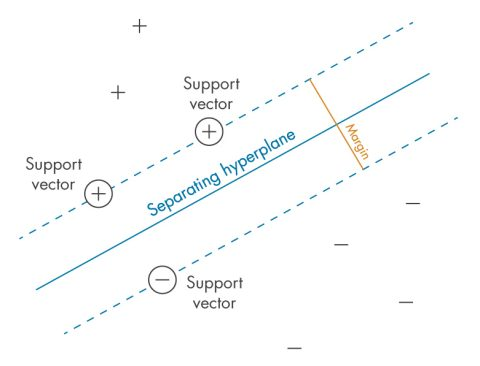
\includegraphics[scale=.6]{support_vector_machine_matlab.jpg}

        {\footnotesize
        Die Trennhyperebene ist in unserem Fall $\langle l,\hat{\mathbb{X}}^{\leq N}_{0,t}\rangle = 1$, die Klasse $\oplus$ ist die Klasse von $l$ mit $\langle l,\hat{\mathbb{X}}^{\leq N}_{0,t}\rangle > 1$ und die Klasse $\ominus$ umgekehrt die mit $\langle l,\hat{\mathbb{X}}^{\leq N}_{0,t}\rangle < 1$.
        \par}
        \label{support_vector_machine}
      \end{figure}
      \newpage

      \subsection{Optimales Stoppen mit Deep Learning}
      % Einleitung und Motivation
      In diesem Unterabschnitt stellen wir die Theorie und das Resultat aus \cite{becker_deep_2019} vor, denn das Konzept der Hybridmethode verfolgt einem ähnlichen Ansatz. Die Optimalität der darin verwendeten Stoppzeit wird hier gezeigt. Das Resultat garantiert ebenfalls die Optimalität der Stoppzeit in der Hybridmethode.
      \hfill\break
      Die Idee von \cite{becker_deep_2019} ist das Lösen des Optimalen Stoppens für markovsche Zufallsprozesse mit einem tief neuronalen Netzwerk. Wir haben das folgende Problem als Ausgangspunkt:
      \begin{align*}
        \underset{\tau \in \mathcal{T}}{sup} \ \mathbb{E}[g(\tau,X_{\tau})],
      \end{align*}
      wobei $X_t$ der Markovprozess, $g$ eine meßbare Abbildung (auch die Auszahlungsfunktion) und $\mathcal{T}$ die Menge der Stoppzeiten ist. Für die numerische Implementierung diskretisiert man die Zeit und setzt $V_n$ als den optimalen Erwartungswert zum Zeitpunkt $n$:
      \begin{align}\label{eqn: becker_V_n}
        V_n = \underset{\tau \in \mathcal{T}_n}{sup} \ \mathbb{E}[g(\tau,X_{\tau})],
      \end{align}
      wobei $\mathcal{T}_n $ die Menge aller Stoppzeiten mit $n \leq \tau \leq N$. Man beachte, dass hier den diskreten Fall untersucht wird und die Stoppzeiten ganzzahlig sind.
      \hfill\break
      Sei $n \in \{ 0,1,\ldots,N-1 \}$ und $f_n,f_{n+1},\ldots,f_N:\mathbb{R}^d \rightarrow \{0,1\}$ mit $f_N \equiv 1 $ eine Folge von meßbaren Funktionen. Man konstruiert die Stoppzeit in $\mathcal{T}_n$ wie folgt:
      \begin{align}\label{eqn: becker_stoppzeit}
        \tau_n = \sum_{m=n}^N mf_m(X_m)\prod_{j=n}^{m-1}(1-f_j(X_j))
      \end{align}
      wobei man hier das leere Produkt $\prod_{j=n}^{m-1}(1-f_j(X_j)) = 1$ setzt.
      \hfill\break
      Im unteren Theorem zeigt man, dass die oben definierte Stoppzeit die Optimalität genügt, d.h. die durch diese Stoppzeit bestimmte Lösung löst das optimale Stoppen (\ref{eqn: becker_V_n}).
      \begin{theorem}\label{theorem: becker_stoppzeit_opt}
        Für gegebene $n \in \{0,1,\ldots,N-1\}$ sei $\tau_{n+1}$ eine Stoppzeit in $\mathcal{T}_{n+1}$ der Form:
        \begin{align*}
          \tau_{n+1} = \sum_{m={n+1}}^N mf_m(X_m)\prod_{j={n+1}}^{m-1}(1-f_j(X_j))
        \end{align*}
        für meßbare Funktionen $f_{n+1},\ldots,f_N:\mathbb{R}^d \rightarrow \{0,1\}$ mit $f_N \equiv 1$. Dann existiert eine meßbare Funktion $f_n: \mathbb{R}^d \rightarrow \{0,1\}$, sodass die durch (\ref{eqn: becker_stoppzeit}) gegebene Stoppzeit $\tau_n \in \mathcal{T}_n$ folgende Ungleichung genügt:
        \begin{align*}
          \mathbb{E}[g(\tau_n,X_{\tau_n})] \geq V_n - (V_{n+1} - \mathbb{E}[g(\tau_{n+1},X_{\tau_{n+1}})]),
        \end{align*}
        wobei $V_n$ und $V_{n+1}$ die definierte Werte in (\ref{eqn: becker_V_n}) sind.
      \end{theorem}
      \begin{beweis-non}
        Appendix \ref{appendix:becker_beweis_iterative_convergence}
        $\hfill\Box$
      \end{beweis-non}

      \begin{bemerkung*}
        \textup{
        Das Resultat bildet die Grundlage für die Optimierung mit der Rückwärtsinduktion. In jedem Schritt $n$ wird die Optimalität von $\tau_n$ gewährleistet. Vergleichbar damit ist die Rückwärtsinduktion aus dem Martingalansatz, wobei man hier keine Folge von Supermartingalen konstruiert. Stattdessen baut man eine Stoppzeit der From (\ref{eqn: becker_stoppzeit}), die man iterativ aktualisiert.
        }
      \end{bemerkung*}
      \hfill\break
      Um die $f_n:\mathbb{R}^d \rightarrow \{0,1\}, \ n=0,1,\ldots,N-1$ numerisch approximieren zu können, verwendet man dazu ein tief neuronales Netzwerk $f^{\theta}:\mathbb{R}^d \rightarrow \{0,1\}$ mit Parameter $\theta \in \mathbb{R}^q$. Im Sinne von (\ref{eqn: becker_stoppzeit}) setzen wir $f^{\theta_N} \equiv 1$ und definieren wir dafür die Stoppzeit zum Zeitpunkt $n+1$:
      \begin{align*}
        \tau_{n+1} = \sum_{m={n+1}}^N mf^{\theta_m}(X_m)\prod_{j={n+1}}^{m-1}(1-f^{\theta_j}(X_j)).
      \end{align*}
      Dabei setzen wir voraus, dass $\theta_{n+1},\theta_{n+2},\ldots,\theta_{N} \in \mathbb{R}^q$ berechnet worden sind. Damit können wir den Erwartungswert $  \mathbb{E}[g(\tau_{n+1},X_{\tau_{n+1}})]$ bestimmen.
      \hfill\break
      Man beachte, dass $f^{\theta}$ Werte in $\{0,1\}$ annimmt. Diese Funktionswerte eignet sich aber nicht für eine gradientenbasierte Optimierungsmethode. Stattdessen approximiert man $f^{\theta}$ mit einem Feedforward neuronalen Netzwerk $F^{\theta}:\mathbb{R}^d \rightarrow (0,1)$ der Form:
      \begin{align*}
        F^{\theta} = \psi \odot a^{\theta}_I \odot \varphi_{q_I-1} \odot a^{\theta}_{I-1} \odot \cdots \odot \varphi_{q_1} \odot a^{\theta}_1,
      \end{align*}
      wobei
    % Die verwendete numerische Methode ist gegeben durch eine iterativ Approximation der optimalen Stopentscheidungen $f_n:\mathbb{R}^d \rightarrow \{0,1\}, \ n=0,1,\ldots,N-1$ mit einem neuronalen Netzwerk $f^{\theta}:\mathbb{R}^d \rightarrow \{0,1\}$ mit Parameter $\theta \in \mathbb{R}^q$. Wie bei der Konstruktion der Stoppzeit fangen wir auch hier mit dem terminalen Stopentscheidung $f_N \equiv 1$ an. Für die Berechnung der weitere Stopentscheidungen führen wir eine Rückwärtsinduktion durch. Sei $ n \in \{ 0,1,\ldots,N-1 \} $ beliebig aber fest. Genauer gesagt, angenommen $\theta_{n+1},\theta_{n+2},\ldots,\theta_{N} \in \mathbb{R}^q$ sind berechnet worden mit $f^{\theta_N} \equiv 1$ und der Stoppzeit
    % \begin{align*}
    %   \tau_{n+1} = \sum_{m={n+1}}^N mf^{\theta_m}(X_m)\prod_{j={n+1}}^{m-1}(1-f^{\theta_j}(X_j)),
    % \end{align*}
    % dann können wir den Erwartungswert $  \mathbb{E}[g(\tau_{n+1},X_{\tau_{n+1}})]$ nahe am Optimum bestimmen. Da $f^{\theta}$ Werte in $\{0,1\}$ annimmt, eignet das Problem sich nicht direkt für eine gradientenbasierte Optimierungsmethode. Stattdessen präsentieren wir ein Feedforward neuronales Netzwerk $F^{\theta}:\mathbb{R}^d \rightarrow (0,1)$ der Form:
    % \begin{align*}
    %   F^{\theta} = \psi \odot a^{\theta}_I \odot \varphi_{q_I-1} \odot a^{\theta}_{I-1} \odot \cdots \odot \varphi_{q_1} \odot a^{\theta}_1,
    % \end{align*}
    % wobei

      \begin{itemize}
        \item $I,q_1,q_2,\ldots,q_{I-1} \in \mathbb{N}$ beschreiben die Tiefe des Netzwerks und die Anzahl der Knoten in den Hidden Layers.
        \item $a_1^{\theta}:\mathbb{R}^d \rightarrow \mathbb{R}^{q_1},\ldots,a_{I-1}^{\theta}:\mathbb{R}^{q_I-2} \rightarrow \mathbb{R}^{q_I-1}$ und $a_{I}^{\theta}:\mathbb{R}^{q_I-1} \rightarrow \mathbb{R}$ sind affine Funktionen.
        \item Für $j \in \mathbb{N}, \varphi_j:\mathbb{R}^j \rightarrow \mathbb{R}^j$ ist die komponentenweise ReLU Aktivierungsfunktion gegeben durch $\varphi_j(x_1,\ldots,x_j)=(x_1^+,\ldots,x_j^+)$.
        \item $\psi:\mathbb{R} \rightarrow (0,1)$ ist die Standard Logistische Funktion mit $\psi (x)=\frac{e^x}{(1+e^x)}=\frac{1}{1+e^{-x}}$
      \end{itemize}
      Der Parameter $\theta \in \mathbb{R}^q$ aus der Funktion $F^{\theta}$ besteht aus den Matrizen $A_1 \in \mathbb{R}^{q_1 \times d},\ldots,A_{I-1} \in \mathbb{R}^{q_{I-1} \times q_{I-2}},A_I \in \mathbb{R}^{1\times q_{I-1}}$ und den Vektoren $b_1 \in \mathbb{R}^{q_1},\ldots,b_{I-1}\in \mathbb{R}^{q_{I-1}},b_I \in \mathbb{R}$. Diese beschreiben die affine Funktionen:
      \begin{align*}
        a_i^{\theta}(x) = A_ix + b_i, \quad i=1,\ldots,I.
      \end{align*}
      Die Dimension des Parameterraums ist gegeben durch:
      \begin{align*}
        q = \begin{cases}
        d+1  &\text{if $I=1$}\\ 1+q_1+\cdots+q_{I-1}+dq_1+\cdots+q_{I-2}q_{I-1}+q_{I-1} &\text{if $I \geq 2$},
      \end{cases}
      \end{align*}
      und für gegebene $x \in \mathbb{R}^d$ ist $\ F^{\theta}(x)$ stetig und fast überall glatt in $\theta$, da die Konstruktion eine Komposition von stetiger Funktionen ist.
      \hfill\break
      Das Ziel ist in jedem Schritt $n$ den Parameter $\theta_n \in \mathbb{R}^q$ so zu bestimmen, sodass
      \begin{align*}
        \mathbb{E}[g(n,X_n)F^{\theta_n}(X_n)+g(\tau_{n+1},X_{\tau_{n+1}})(1-F^{\theta_n}(X_n))]
      \end{align*}
      in einer hinreichend kleinen Umgebung des Supremums
      \begin{align}\label{eqn: becker_functional}
        \underset{\theta \in \mathbb{R}^q}{sup} \ \mathbb{E}[g(n,X_n)F^{\theta}(X_n)+g(\tau_{n+1},X_{\tau_{n+1}})(1-F^{\theta}(X_n))]
      \end{align}
      liegt, welcher einem eine gute Approximation von (\ref{eqn: becker_functional}) liefert. Wenn das erreicht wird und $\theta_n$ bestimmt ist, setzt man die Funktion $f^{\theta_n}: \mathbb{R}^d \rightarrow \{0,1\}$ als:
      \begin{align}\label{dnn_function_f}
        f^{\theta_n} = \mathds{1}_{[0,\infty)}\odot a_I^{\theta_n} \odot \varphi_{q_{I-1}} \odot a_{I-1}^{\theta_n} \odot \cdots \odot \varphi_{q_{1}} \odot a_{1}^{\theta_n}.
      \end{align}
      Der einzige Unterschied zwischen $F^{\theta_n}$ und $f^{\theta_n}$ ist die letzte Funktion: $F^{\theta_n}$ gibt mit der logistischen Funktion einen Wert aus $(0,1)$ zurück, und $f^{\theta_n}$ eine Zahl aus der Menge $\{0,1\}$.
      \hfill\break
      Im folgenden Resultat zeigt man die Optimalität des oben konstruierten tief neuronalen Netwerks. Für jede Tiefe $I \geq 2$ ist die Approximation des neuronalen Netzwerks der Form (\ref{dnn_function_f}) so gut, dass das Funktional (\ref{eqn: becker_functional}) in einer $\varepsilon$ Umgebung von dem durch $f$ definiertes Funktional liegt, wenn man dem neuronalen Netzwerk $F^{\theta}$ hinreichend viele Knoten zur Verfügung stellt.
      \begin{lemma}\label{becker: beweis_ineq}
        \textup{
        Sei $n \in \{ 0,1,\ldots,N-1 \}$ und fixiere die Stoppzeit $\tau_{n+1} \in \mathcal{T}_{n+1}$. Dann gilt für jede Tiefe $I \geq 2$ und konstante $\varepsilon > 0$, dass es natürliche Zahlen $q_1,\ldots,q_{I-1} \in \mathbb{N}$ gibt mit:
        \begin{align*}
          & \underset{\theta \in \mathbb{R}^d}{sup} \ \mathbb{E}[g(n,X_n)f^{\theta}(X_n)+g(\tau_{n+1},X_{\tau_{n+1}})(1-f^{\theta}(X_n))] \\
          & \geq \underset{f \in \mathcal{D}}{sup} \ \mathbb{E}[g(n,X_n)f(X_n)+g(\tau_{n+1},X_{\tau_{n+1}})(1-f(X_n))] - \varepsilon,
        \end{align*}
        wobei $\mathcal{D}$ die Menge aller messbare Funktionen $f: \mathbb{R}^d \rightarrow \{0,1\}$
        }
      \end{lemma}
      \begin{beweis-non}
        Appendix \ref{appendix:becker_beweis_ineq}
      \end{beweis-non}
      \hfill\break
      Der Kanditat für die optimale Stoppzeit ist
      \begin{align}\label{eqn: becker_optimal_stopping_time}
        \tau^{\Theta} = \sum_{n=1}^{N}n f^{\theta_n}(X_n)\prod_{j=0}^{n-1}(1-f^{\theta_j}(X_j))
      \end{align}
      wobei $\Theta = (\theta_0,\theta_1,\ldots,\theta_{N-1}) \in \mathbb{R}^{N_q}$ ein Vektor für alle Parameter ist.
      \hfill\break
      Für das numerische Experiment hat man die neuronale Netzwerke der Form (\ref{dnn_function_f}) mit fester Tiefe $I \geq 2$ und mit der Anzahl $q_1,\ldots,q_{I-1}$ an Knoten für die jeweilige Hidden Layers gewählt. Um die Parameter $\theta_n \in \mathbb{R}^q$ in allen Zeitpunkten numerisch zu bestimmen, approximiert man den Erwartungswert in (\ref{eqn: becker_functional}) mithilfe von Monte Carlo Approximation.
      \hfill\break
      Man initialisiert $\theta_N \in \mathbb{R}^q$ mit $f^{\theta_N} \equiv 1$ und bestimmt alle $\theta_n \in \mathbb{R}^q, 1 \leq n \leq N-1$ rekursiv. Angenommen, dass für gegebene $n \in \{0,1,\ldots,N-1\}$ die Parameter $\theta_{n+1},\ldots,\theta_N \in \mathbb{R}^q$ berechnet worden sind und die Stopentscheidungen $f^{\theta_{n+1}},\ldots,f^{\theta_N}$ die folgende Stoppzeit definiert:
      \begin{align*}
        \tau_{n+1} = \sum_{m={n+1}}^N mf^{\theta_m}(X_m)\prod_{j={n+1}}^{m-1}(1-f^{\theta_j}(X_j))
      \end{align*}
      mit entsprechendem Erwartungswert $\mathbb{E}g(\tau_{n+1},X_{\tau_{n+1}})$. Um $\theta_n$ zu bestimmen, löst man dazu:
      \begin{align*}
        \underset{\theta \in \mathbb{R}^q}{sup} \ \mathbb{E}[g(n,X_n)F^{\theta}(X_n)+g(\tau_{n+1},X_{\tau_{n+1}})(1-F^{\theta}(X_n))].
      \end{align*}
      Für das Lösen von $g(n,X_n)F^{\theta}(X_n)+g(\tau_{n+1},X_{\tau_{n+1}})(1-F^{\theta}(X_n))$ verwendet man eine gradientenbasierte Optimierungsmethode und für die Approximation des Erwartungswerts die Monte-Carlo Methode. Den daraus resultierenden Parameter $\theta_n^*$ setzen wir in die Stoppentscheidung $f^{\theta_n}$ ein und erhalten die Stoppzeit zum Zeitpunkt $n$:
      \begin{align*}
        \tau_{n} = \sum_{m={n}}^N mf^{\theta_m}(X_m)\prod_{j={n}}^{m-1}(1-f^{\theta_j}(X_j))
      \end{align*}
      Nach dem Durchlauf aller Zeitpunkten erhalten wir die berechnete Parameter für $\Theta$ und damit auch den Kandidaten der optimalen Stoppzeit (\ref{eqn: becker_optimal_stopping_time}).
      % der in der Nähe des optimalen Wertes $V_{n+1}$ liegt. Für $n=N-1$ hat man $\tau_{n+1} \equiv N$ und für $n \leq N-2$ hat man:
      % \begin{align*}
      %   \tau_{n+1} = l_{n+1}(X_{n+1},\ldots,X_{N-1}),
      % \end{align*}
      % wobei $l_{n+1}:\mathbb{R}^{N-n-1} \rightarrow \{ n+1, n+2, \ldots, N\}$ messbare Funktionen sind. Entsprechend schreiben wir:
      % \begin{align*}
      %   l_{n+1}^k \begin{cases}
      %     N  &\text{if $n=N-1$}\\
      %     l_{n+1}(x_{n+1}^k,\ldots,x_{N-1}^k) &\text{if $n \geq N-2$}.
      %   \end{cases}
      % \end{align*}
      % Wenn man zum Zeitpunkt $n$ die Soft-Stopentscheidung $F^{\theta}$ anwendet und sich danach gemäß $f^{\theta_{n+1}},\ldots,f^{\theta_N}$ verhält, ist der realisierte Reward entlang des k-ten simulierten Pfades von $X$:
      % \begin{align*}
      %   r_n^k(\theta) = g(n,x_n^k)F^{\theta}(x_n^k)+g(l_{n+1}^k,x_{l_{n+1}^k}^k)(1-F^{\theta}(x_n^k)).
      % \end{align*}
      % Für $K \in \mathbb{N}$ groß genug approximiert
      % \begin{align*}
      %   \frac{1}{K}\sum_{k=1}^Kr_n^k(\theta)
      % \end{align*}
      % den Erwartungswert
      % \begin{align*}
      %   \mathbb{E}[g(n,X_n)F^{\theta}(X_n)+g(r_{n+1},X_{r_{n+1}})(1-F^{\theta}(X_n))].
      % \end{align*}
      % Diese Approximation heißt \textit{Monte Carlo Simulation} und wird in Appendix \ref{appendix:mc-methode} in Details aufgeführt.
      % Da $r_n^k(\theta)$ in $\theta$ fast überall differenzierbar ist, verwenden wir das Stochastisches Gradientenverfahren, um den approximierten Optimierer $\theta \in \mathbb{R}^q$ zu finden. Die gleiche Simulationen $(x_n^k)_n=0^N$ kann auch für das Trainieren der Stopentscheidungen $f^{\theta_n}$ zu jedem Zeitpunkt $n \in \{0,1,\ldots,N-1 \}$ verwendet werden.
      % \begin{bemerkung*}
      %   \textup{
      %   Wenn ein Markovprozess $X$ von einem deterministischen Anfangswert $x_0 \in \mathbb{R}^d$ anfängt, dann ist die Anfangsstopentscheidung durch eine Konstante $f_0 \in \{0,1\}$ gegeben. Um $f_0$ durch die simulierten Pfade von $X$ zu bestimmen, reicht es aus, wenn wir den Anfangsreward $g(0,x_0)$ mit einer Monte Carlo Schätzung $\hat{C}$ von $\mathbb{E}[g(\tau_1,X_{\tau_1})]$ vergleichen, wobei $\tau_1 \in \mathcal{T}_1$ ist und die folgende Form annimmt:
      %   \begin{align*}
      %     \tau_1 = \sum_{n=1}^Nnf^{\theta_n}(X_n)\prod_{j=1}^{n-1}(1-f^{\theta_j}(X_j))
      %   \end{align*}
      %   für $f^{\theta_N} \equiv 1$ und Trainingsparameter $\theta_1,\ldots,\theta_{N-1} \in \mathcal{R}^q$. Dann kann man $f_0 = 1$ setzen, d.h. der Prozess stoppt gleich am Anfang, falls $g(0,x_0) \geq \hat{C}$ und $f_0 = 0$, d.h. der Prozess stoppt nicht und setzt fort. Die resultierende Stoppzeit hat die Form:
      %   \begin{align*}
      %     \tau^{\Theta} =
      %     \begin{cases}
      %       0 &\text{if $f_0 = 1$}\\
      %       \tau_1 &\text{if $f_0 = 0$}.
      %     \end{cases}
      %   \end{align*}
      %   }
      % \end{bemerkung*}
      % \begin{beispiel}[Bermudan Max-Call Option]
      %   \hfill\break
      %   \textup{
      %   Als erstes Beispiel betrachten wir die Bepreisung einer Bermudan Max-Call Option. Diese Option ist eine der meist studierte Beispiele in der numerischen Literaturen von Optimalem Stopproblem \cite{longstaff_valuing_2001; rogers_monte_nodate; garcia2003convergence, Bboyle2003improved}. Deren Payoff hängt von dem Maximum der $d$ zugrundeliegende Basisaktien.
      %   Angenommen, die risiko-neutrale Dynamiken der Aktien sind durch multi-dimensionales Black Scholes Modell gegeben:
      %   \begin{align*}
      %     S_t^i = s_0^i exp((r-\delta_i-\sigma_i^2/2)t+\sigma_i^2W_t^i), \quad i=1,2,\ldots,d,
      %   \end{align*}
      %   wobei $s_0^i \in (0,\infty)$ der Anfangswert, $r \in \mathbb{R}$ die risiko-neutrale Zinsrate, $\delta_i \in [0,\infty)$ die Dividendenrate, $\sigma_i \in (0,\infty)$ und $W$ die d-dimensionale Brownsche Bewegung mit konstanten momentanen Korrelationen $\rho_{ij} \in \mathbb{R}$ zwischen verschiedenen Komponenten $W^i$ und $W^j$ für $i\neq j$ ist.
      %   Eine Bermudan max-call Option auf $S^1,\ldots,S^d$ hat die Auszahlungsfunktion $(\underset{1\leq i \leq d}{max} \ S^i_t-K)^+$ und kann zu jedem diskreten Zeitpunkt $0=t_0 < t_1 < \ldots < t_N$ ausgeführt werden. Das Preisprofil ist gegeben durch:
      %   \begin{align*}
      %     \underset{\tau}{sup} \ \mathbb{E}[e^{-r\tau} (\underset{1\leq i \leq d}{max} \ S^i_t-K)^+],
      %   \end{align*}
      %   wobei das Supremum über alle $S$-Stoppzeiten mit Werten in $\{t_0,t_1,\ldots,t_N\}$ ist \cite{schweizer2002bermudan}. Wir schreiben $X_n^i = S_{t_n}^i, \ n=0,1,\ldots,N$ und definieren $\mathcal{T}$ als die Menge aler $X$-Stoppzeiten. Dann kann der Optionspreis als $\underset{\tau \in \mathcal{T}}{sup} \ \mathcal{E}[g(\tau,X_{\tau})] $ geschrieben werden mit:
      %   \begin{align*}
      %     g(n,x) = e^{-rt_n}(\underset{1\leq i \leq d}{max} \ x^i -K )^+.
      %   \end{align*}
      %   Für die numerische Untersuchung diskretisieren wir das Zeitinterval durch $t_n = nT/N, n=0,1,\ldots,N$ für jede Fälligkeit $T>0$ und $N+1$ äquidistante Ausübungszeitpunkte. Der Markovprozess $Y_n$ ist definiert durch $(Y_n)_{n=0}^N = (X_n,g(n,X_n))_{n=0}^N$. Da $Y_0$ deterministisch ist, können wir die erste Stoppzeit $\tau_1 \in \mathcal{T}$ trainieren durch:
      %   \begin{align*}
      %     \tau_1 = \sum_{n=1}^N nf^{\theta_n}(Y_n)\prod_{j=1}^{n-1}(1-f^{\theta_j}(Y_k))
      %   \end{align*}
      %   für $f^{\theta_N} \equiv 1$ und $f^{\theta_1},\ldots,f^{\theta_{N-1}}:\mathcal{R}^{d+1} \rightarrow \{0,1\}$ mit $I=2$ und $q_1=q_2=d+40$. Dann ist der Kandidat für die optimale Stoppzeit bestimmt durch:
      %   \begin{align*}
      %     \tau^{\Theta}
      %     \begin{cases}
      %       0 &\text{if $f_0 = 1$}\\
      %       \tau_1 &\text{if $f_0 = 0$}.
      %     \end{cases}
      %   \end{align*}
      %   für eine Konstante $f_0 \in \{0,1\}$.
      %   Für eine gute Vergleichbarkeit dieser Methode und unserer Methoden verwenden wir für die Simulation folgende Konstante: sei $i=1,\ldots,d$, wir setzen:
      %   \begin{align*}
      %     x_0^i = 90, \quad K=100, \quad \sigma_i = 20\%, \quad \delta_i = 10\%, \quad r=5\%, \quad T=3, \quad N=9.
      %   \end{align*}
      %   Damit simulieren wir die Aktienpreise durch:
      %   \begin{align*}
      %     x_{n,i}^m = x_{0,i} \dot exp(\sum_{k=0}^n ((r-\delta_i-\sigma_i^2/2)\Delta t + \sigma_i \sqrt{\Delta t} \dot Z_{k,i}^m)),
      %   \end{align*}
      %   wobei $\Delta t=T/N$ und $Z_{k,i}^m \sim \mathcal{N}(0,1)$
      %   \textcolor{red}{das muss ich noch implementieren!!!}
      %   \textcolor{red}{die haben noch das ganze in symmetrischen Fall und asymmetrischen Fall unterschieden. Auswertungen gibt es als Tabellen, miteinbeziehen?}
      %   }
      % \end{beispiel}
      \begin{beispiel}[fraktionale Brownsche Bewegung]\label{bsp: becker_fbm}
        \textup{
        Für die numerische Experimente hat man in \cite{becker_deep_2019} die fraktionale Brownsche Bewegung gewählt.
        % Eine fraktionale Brownsche Bewegung mit Hurst Parameter $H \in (0,1]$ ist ein zentrierter stetiger Gaussprozess $(B_t^H)_{t \geq 0}$ mit der Kovarianz:
        % \begin{align*}
        %   \mathbb{E}[B_t^HB_s^H]=\frac{1}{2}(t^{2H}+s^{2H}-{\lvert t-s \rvert}^{2H}).
        % \end{align*}
        % Für $H = 1/2$ ist $B_t^H$ die Standard Brownsche Bewegung. Gemäß des Optimal Stopping Theorems ist $\mathbb{E}[B_t^{1/2}]=0$ für jede nach oben beschränkte $B^{1/2}$-Stoppzeit $\tau$\cite{grimmett2020probability}. Für $H \neq 1/2$ sind die Inkremente von $B^H$ für $H \in (1/2,1]$ positiv korreliert und für $H \in (0,1/2)$ negativ korreliert. In beiden Fällen ist $B_t^H$ weder ein Martingal noch ein Markovprozess und es exisiteren $B^H$-Stoppzeiten $\tau$ mit $\mathbb{E}[B_{\tau}^H]>0$ (siehe \cite{Kulikov and Gusyatnikov (2016)})
        Um das optimale Stoppen
        \begin{align*}
          \underset{0\leq \tau \leq 1}{sup} \ \mathbb{E}[B_{\tau}^H]
        \end{align*}
        über alle $B^H$-Stoppzeiten $\tau \in [0,1]$ zu lösen, diskretisiert man zunächst das Zeitinterval $[0,1]$ mit $t_n=n/100, \ n=0,1,\ldots,100$. Das führt zu der Konstruktion des Markovprozesses $(W_n)_{n=0}^{100}$:
        \begin{align*}
          W_0 &= (0,0,\ldots,0) \\
          W_1 &= (B_{t_1}^H,0,\ldots,0) \\
          W_2 &= (B_{t_2}^H,B_{t_1}^H,0,\ldots,0) \\
          & \vdots \\
          W_{100} &= (B_{t_{100}}^H,B_{t_{99}}^H,\ldots,B_{t_1}^H) \\
        \end{align*}
        Damit wendet man das Resultat auf
        \begin{align}\label{eqn: becker_os_fbm}
          \underset{\tau \in \mathcal{T}}{sup} \mathbb{E}[g(W_{\tau})]
        \end{align}
        an. Man beachte, dass (\ref{eqn: becker_os_fbm}) $\underset{0\leq \tau \leq 1}{sup} \ \mathbb{E}[B_{\tau}^H]$ von unten approximiert, wobei $\mathcal{T}$ die Menge aller $X$-Stoppzeiten ist und $g:\mathbb{R}^{100} \rightarrow \mathbb{R}$ die Projektion $(x^1,\ldots,x^{100}) \mapsto x^1$ ist.
        }
      \end{beispiel}
      \begin{bemerkung*}
        \textup{
        Dieser Ansatz für das Lösen des optimalen Stoppen motiviert unsere Idee für die Hybridmethode. Wir verwenden die im Theorem (\ref{eqn: main_equality}) definierte Klasse von Signatur Stoppzeiten anstatt ein tiefneuronales Netzwerk. Genauer gesagt ersetzen wir das Netzwerk durch die Hyperebene $\langle l, \hat{\mathbb{X}}^{\leq N}_{0,t_n} \rangle - 1$. Der Trainingsprozess sowie die Struktur des Kanditaten für die optimale Stoppzeit haben wir angepasst.
        }
      \end{bemerkung*}
      \newpage

      \subsection{Hybridmethode}

      Eine weitere von uns untersuchte Methode ist die Hybridmethode. Wir geben ihr den Namen, da diese das Konzept der Signaturmethode und das von dem Resultat aus \cite{becker_deep_2019} kombiniert. Die Idee besteht darin, dass wir für jeden diskreten Zeitpunkt ein lokales $l \in \mathcal{T}((\mathbb{R}^{1+d})^*)$ statt ein globales $l$ für alle Signaturen zu jedem Zeitpunkt bestimmen. Dabei haben wir uns auf das Konzept von \cite{becker_deep_2019} orientiert. Dort hat man die Stoppentscheidungen mit mit einem tief neuronalen Netzwerk $f^{\theta}$ approximiert und dies mit einem Recurrent neuronalen Netzwerk $F^{\theta}$ abgeschätzt, indem man die Parameter $\theta$ durch die Optimierung des Funktionals (\ref{eqn: becker_functional}) bestimmt.
      \hfill\break
      Wir betrachten dagegen die Signatur von dem stochastischen Prozess und konstruieren damit die Stoppentscheidungen $f_n^l(\hat{\mathbb{X}}^{\leq N})$ werden durch
      $F_n^l(\hat{\mathbb{X}}^{\leq N}) := \psi( \langle l, \hat{\mathbb{X}}^{\leq N}_{0,t_n} \rangle - 1)$ approximiert. Das bedeutet, wir haben anstelle von dem Recurrent neuronalen Netzwerk die Hyperebene $\langle l, \hat{\mathbb{X}}^{\leq N}_{0,t_n} \rangle - 1$ in der Definition (\ref{def: class_l}) für die Signatur Stoppzeit verwendet. Somit optimieren wir die
      $F_n^l$ über $l$ mit dem Funktional
      \begin{align*}
        \underset{l \in \mathcal{T}((\mathbb{R}^{1+d})^*)}{argmax} \ \mathbb{E}[g(t_n, Y_{t_n})F_n^l(\hat{\mathbb{X}}^{\leq N})+g(\tau_{n+1},Y_{\tau_{n+1}})(1-F_n^l(\hat{\mathbb{X}}^{\leq N})) ].
      \end{align*}
      \hfill\break
      Wir gehen wie folgt vor: sei $0=t_0<t_1<\ldots<t_K=1$. Wir suchen nach der optimalen Stoppzeit $\tau^*$ für V mit:
      \begin{align*}
        V = \underset{\tau}{sup} \ \mathbb{E}[g(\tau,Y_{\tau})].
      \end{align*}
      \hfill\break
      Sei weitherhin $\mathcal{T}_n, \ n \in \{0,\ldots,K\}$ die Menge der Stoppzeiten zum Zeitpunkt $n$ mit Werten aus $\{ t_n, t_n+1,\ldots,t_K \}$ und
      \begin{align*}
        f^l_n(\hat{\mathbb{X}}^{\leq N}) = \mathds{1}_{ \{ \langle l, \hat{\mathbb{X}}^{\leq N}_{0,t_n}  \rangle \geq 1 \} }
      \end{align*}
      die modifizierte Stoppentscheidungsfunktion. Wir sind an Stoppzeiten der Form interessiert:
      \begin{align*}
        \tau := \sum_{n=1}^K t_nf_n^{l_n}(\hat{\mathbb{X}}^{\leq N})\prod_{j=0}^{n-1}(1-f_j^{l_j}(\hat{\mathbb{X}}^{\leq N}))
      \end{align*}
      Die Meßbarkeit bzgl. $\mathcal{F}_t$ der so definierte Stoppzeit ist durch die $\mathcal{F}_t$-Meßbarkeit von $\hat{\mathbb{X}}^{\leq N}_t$ gegeben. Um $f_n^l$ abzuschätzen, verwenden wir $F_n^l$:
      \begin{align*}
        F_n^l(\hat{\mathbb{X}}^{\leq N}) = \psi( \langle l, \hat{\mathbb{X}}^{\leq N}_{0,t_n} \rangle - 1),
      \end{align*}
      wobei $\psi(x) = \frac{1}{1+e^{-x}}$ die logistische Funktion ist. Wir ersetzen also das Recurrent neuronales Netzwerk durch unsere Hyperebenegleichung.
      %Die daraus resultierende Stoppzeit ist im Vergleich zu der Signaturmethode keine Eintrittszeit einer Hyperebene, denn diese ist eine Komposition von mehreren Stopentscheidungen. Diese werden in jedem diskreten Zeitpunkt durch die Eintrittszeit der Hyperebene $\langle l_n^*, \hat{\mathbb{X}}^{\leq N}_{0,t_n}  \rangle \geq 1$ bestimmt.
      \hfill\break
      Wie in \cite{becker_deep_2019} führen wir für die Berechnung von $l$ die Rückwärtsinduktion durch:
      \begin{itemize}
        \item Wir initialisieren $f_K^{l_K} \equiv 1$ und $\tau_K=1 \in \mathcal{T}_K$.
        \item Sei $n \in \mathbb{N}$ mit $n \leq N-1$ beliebig aber fest. Angenommen, wir haben $l_{n+1},\ldots,l_N$ gefunden und somit auch die Stoppzeiten $\tau_{n+1},\tau_{n+2},\ldots,\tau_{N}$. Die haben jeweils die Form:
        \begin{align*}
          \tau_{u} = \sum_{m=u}^K t_mf_m^{l_m}(\hat{\mathbb{X}}^{\leq N})\prod_{j=u}^{m-1}(1-f_j^{l_j}(\hat{\mathbb{X}}^{\leq N})) \in \mathcal{T}_{u}.
        \end{align*}
        für $u \in \{n+1,\ldots,N\}$. Man beachte, dass auch bei uns das leere Produkt $\prod_{j=u}^{m-1}(1-f_j^{l_j}(\hat{\mathbb{X}}^{\leq N})) = 1$ definiert ist für $u>m-1$.
        \item Für die Bestimmung von $\tau_n$ lösen wir dazu das Optimierungsproblem
        \begin{align}\label{eqn: l_n}
          l_n^* = \underset{l}{argmax} \ \mathbb{E}[g(t_n, Y_{t_n})F_n^l(\hat{\mathbb{X}}^{\leq N})+g(\tau_{n+1},Y_{\tau_{n+1}})(1-F_n^l(\hat{\mathbb{X}}^{\leq N})) ],
        \end{align}
        welches uns das optimale $l_n^*$ liefert.
        \item Mit dem berechneten $l_n^*$ definieren wir die Stopentscheidung $f_n^{l_n^*} := \mathds{1}_{ \{ \langle l_n^*, \hat{\mathbb{X}}^{\leq N}_{0,t_n}  \rangle \geq 1 \} }$ zum Zeitpunkt $t_n$. Damit erhalten wir die Stoppzeit $\tau_n$:
        \begin{align*}
          \tau_{n} = \sum_{m=n}^K t_mf_m^{l_m}(\hat{\mathbb{X}}^{\leq N})\prod_{j=n}^{m-1}(1-f_j^{l_j}(\hat{\mathbb{X}}^{\leq N})).
        \end{align*}
        \item Nach dem Durchlauf aller Zeitpunkte erhalten wir die so berechtete optimale Stoppzeit und diese nimmt die Form an:
        \begin{align*}
          \tau^* = \sum_{n=1}^K t_nf_n^{l_n}(\hat{\mathbb{X}}^{\leq N})\prod_{j=0}^{n-1}(1-f_j^{l_j}(\hat{\mathbb{X}}^{\leq N}))
        \end{align*}
      \end{itemize}
      Für die Bestimmung von $l_n$ in der Gleichung (\ref{eqn: l_n}) wenden wir zunächst die Monte-Carlo Methode für die Approximation des Erwartungswerts und Gradient Descent Methode für die Bestimmung der optimalen Lösung $l^*_n$ an.
      %Wir haben in unserem Optimierungsproblem stochastische Größen, was das Problem zu einem stochastischen Optimierungsproblem umwandelt. Daher eignet sich die Monte Carlo Methode besonders gut für die Approximation des Erwartungswerts in \ref{eqn: l_n}.
      Eine Einführung in die Monte Carlo Methode findet man in Appendix \ref{appendix:mc-methode}. Die konventionelle Gradient Descent Methode hat in unserem Fall schlecht performt, da die Gradienten von dem zu optimierenden Funktional in (\ref{eqn: l_n)} dünn besetzt ist und somit die Änderung pro Schritt sehr klein ist. In manchen Fällen konvergiert die Methode gar nicht gegen einen Punkt. Stattdessen springen die Werte in einem kleinen Bereich hin und her. Da das Problem in vielen Deep Learning Optimierungsproblemen auch vorkommt, haben wir als Ausweg die Adam Methode \cite{kingma_adam_2017} gewählt. Die Kernidee von Adam ist die Schätzung der ersten und zweiten Momente vom Gradient des Funktionals und die Verwendung solcher Schätzungen in der Schrittweite. Dadurch ermöglicht die Adam Methode einem, dass Schrittweite in jedem Iterationsschritt individuell gesetzt werden. Eine ausführliche Einführung in die Methode haben wir in Appendix \ref{appendix: adam method} verfasst.
      \begin{bemerkung*}
        \textup{
        Nachdem wir die Idee von \cite{becker_deep_2019} zur Motivation der Hybridmethode eingeführt und das Konzept unserer beiden Methoden vorgestellt haben, werden wir im nächsten Abschnitt die experimentellen Resultaten auswerten und darüber diskutieren. Wir geben bekannt, unter welchen Bedingungen an Hardwares und Softwares wir die Experimente durchgeführt haben und welche Einschränkung diese Bedingungen uns verursacht haben. Eine Auswertung der Relation zwischen dem Hurstparameter und dem optimal gestoppten Erwartungswert für fraktonale Brownsche Bewegungen wie in \cite{becker_deep_2019} haben wir ebenfalls für die Signaturmethode und die Hybridmethode erstellt.
        }
      \end{bemerkung*}

      \newpage

      % \section{Experimentelle Resultate}
      % \textcolor{red}{wird am Samstag der 11.09.2021 geschrieben} In diesem Kapitel werden die Resultate der Simualtion ausgewertet und auf Pro und Contra diskutiert. (kann auch mit dem obigen Kapitel zusammengeführt werden).
      % \begin{itemize}
      %   \item Beschreibung unserer Resultate
      %   \item Vergleich mit dem von Becker
      %   \item Mögliche Verbesserung bzw. was würde ich in der Zukunft verbessern
      % \end{itemize}
      % Inhalt:
      % \begin{itemize}
      %   \item wir haben wie in dem Paper von Becker \cite{becker_deep_2019} die Wertefunktion mit dem Hurstparameter verglichen. Dabei stellt es sich heraus, dass das asymptotisches Verhalten von der Wertefunktion bzgl. des Hurstparameters bis zum Punkt 0 bei beiden Untersuchungen nahezu identisch ist. Siehe Graphen \textit{DOS} und \textit{my-plot}. \textcolor{red}{soll ich hier den orangen Graphen erwähnen und beschreiben?}
      %   \item in dem Beispiel "Bermudan Option" sehen wir ebenfalls:
      %   \begin{itemize}
      %     \item wie sieht die Stopregel hier aus?
      %     \item welche Methode weist einen größeren Wertefunktion auf?
      %     \item welche Methode hat kürzere Berechnungszeit?
      %     \item welche Indikatoren kann man noch vergleichen?
      %   \end{itemize}
      %   \item benötigte Graphen:
      %   \begin{itemize}
      %     \item Expect vs. Hurst bei der Signatur Methode
      %     \item Graphen für die Bermudan Option
      %     \item Tabelle für die Trainingszeit bei verschied. N
      %     \item Expect vs. Hurst bei Deep Signatur Methode (dafür muss ich den Programm über Nacht laufen lassen.)
      %   \end{itemize}
      % \end{itemize}
      %
      % \newpage

    \section{Diskussionen und Limitationen}
      In diesem Abschnitt werten wir die Ergebnisse aus der numerischen Implementierung aus. Als Testobjekt haben wir die fraktionale Brownsche Bewegung ausgewählt, da diese weder ein Markovprozess noch ein Martingal ist. Als Benchmark verwenden wir das Resultat aus \cite{becker_deep_2019} für das Testobjekt und messen ebenfalls die Relation zwischen dem Hurstparameter und $\underset{\tau \in \mathcal{T}}{sup} \mathbb{E}[Y_{\tau}]$. Die Qualität der Methode ist durch die Messungen reflektiert. Dabei vergleichen wir sowohl die Werte als auch den Verlauf der gemessenen Daten.
      \hfill\break
      Im Anschluss diskutieren wir die Vor- und Nachteile der Signatur- und Hybridmethode. Mögliche Ideen für weitere Forschung werden ebenfalls genannt.
      \subsection{Experimentaufbau}
      % Resultat von Becker
      In \cite{becker_deep_2019} hat man für die numerische Implementierung eine Stichprobenanzahl von $M = 30'000$ verwendet. Für die Erstellung der Abbildung (\ref{fig: becker_expec_vs_hurst}) berechnet man für $H \in \{0.01,0.05,0.1,0.15,\ldots,1\}$ einzeln die optimale Stoppzeit $\tau^*$ und bestimmt dann den Wert von $\mathbb{E}[B_{\tau^*}^H]$. Für
      $H=1/2$ haben wir die Brownsche Bewegung. Theoretisch ist $\mathbb{E}[B^{1/2}_{\tau}] = 0$ und in der Abbildung ist diese Aussage bestätigt. Für $H = 1$ hat man $B_t^1 = tB_{t_1}^1$. In diesem Fall ist die optimale Stoppzeit gegeben durch
      \begin{align*}
        \tau =
        \begin{cases}
          1 & \textup{falls } B_{t_1}^1 > 0 \\
          t_1 & \textup{falls } B_{t_1}^1 \leq 0
        \end{cases}
      \end{align*}

      \begin{figure}[H]
        \caption{Deep Optimal Stopping \cite{becker_deep_2019}}
        \centering
        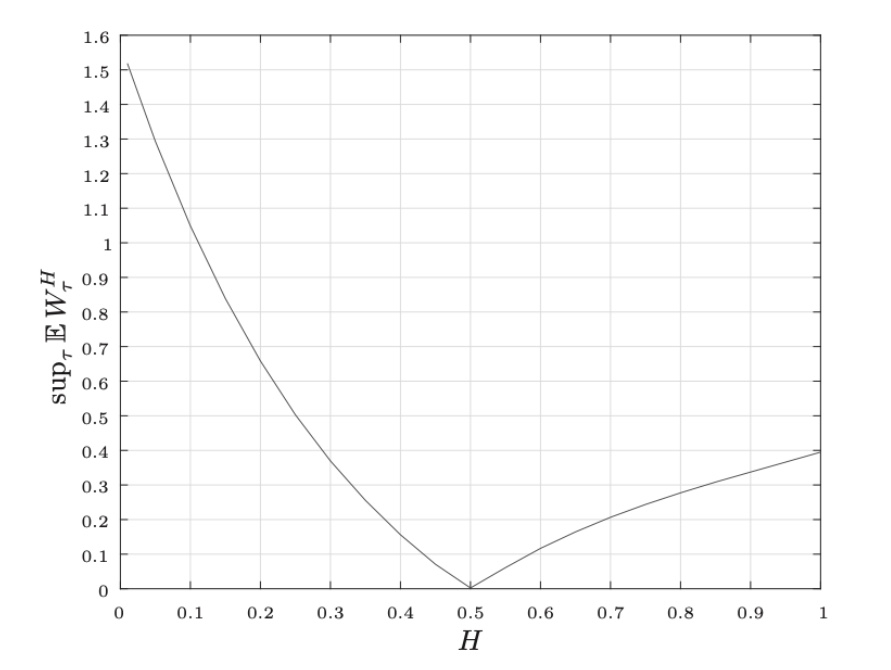
\includegraphics[width=0.9\textwidth]{becker_expec_vs_hurst.jpg}
        {\footnotesize
        \hfill\break
        $W_t^H$ ist hier im Beispiel (\ref{bsp: becker_fbm}) konstruierter Markovprozess.
        \par}
        \label{fig: becker_expec_vs_hurst}
      \end{figure}
      \hfill\break
      % Hardware und Software
      Für unsere Implementierung haben wir als Hardware das \textit{Raspberry Pi 4} mit 4 GB RAM und einem CPU mit 4 Cores verwendet. Die Entwicklungsumgebung ist das \textit{JupyterLab}. Das ist eine Erweiterung von Jupyter Notebook in Python, womit man zusätzliche IT-technische Einstellungen tätigen kann. Für die Generierung der Stichproben benutzen wir \texttt{fbm \footnote{https://pypi.org/project/fbm/}} und für die grundlegende Berechnung und die Speicherung von Daten \texttt{numpy \footnote{https://pypi.org/project/numpy/}}.
      \hfill\break
      Sei $x_1,\ldots,x_M \in \mathbb{R}^{d \times K}$ die generierte Stichproben mit der Dimension $d$ und der Anzahl an diskrete Zeitpunkte $K$. Die Stichproben werden stets mit der Dimension $d=1$ und $K=100$ generiert. Man beachte, dass wir für unsere Berechnung den erweiterten Prozess betrachten, d.h. $\hat{X}_t = (t,X_t)$. Dann ist die Datenmatrix gegeben durch
      $\mathbb{D} = [x_1^T,\ldots,x_M^T] \in \mathbb{R}^{K \times M \times ({d+1}})$. Der Zeithorizont ist bei uns in beiden Methoden $T=1$. Für die Berechnung der Signatur verwenden wir \texttt{iisignature \footnote{https://pypi.org/project/iisignature/}}. Das Niveau für die geschnittete Signatur setzen wir in beiden Fällen auf $N=8$. Zusätzlich haben wir in den Graphen wegen der kleinen Datenmengen die Trendlinie gezeichnet, welche durch Interpolation von Polynomen $3.$ Grades erzeugt wurde, um den Verlauf beider Messungen mit dem Graphen in Fig: (\ref{fig: becker_expec_vs_hurst}) besser vergleichen zu können.
      \hfill\break
      In den Beispielen (\ref{rough_path: brownian_motion}) und (\ref{rough_path: fbm}) haben wir gezeigt, dass die Brownsche Bewegung und die fraktionale Brownsche Bewegung zu Rough Path erweitert werden. Sowohl für die Brownsche Bewegung als auch für die fraktionale Brownsche Bewegung können wir die Theorie der Rough Paths bis hinzu die Resultate für die Signaturen Stoppzeit verwenden.
      \hfill\break
      % Resultat aus der Signaturmethode
      Wir nutzen für die Erstellung von Fig: (\ref{fig: signatur_methode}) für die Signaturmethode eine Trainingsstichprobengröße von $M_{train}=15'000$ und eine Teststichprobengröße von $M_{test}=5'000$. Weiterhin berechnen wir für $H \in \{0.02,0.03,\ldots,0.98,0.99\}$ jeweils den Wert für $\mathbb{E}[Y_{\tau}]$. Eine Darstellung findet man in Fig:
      (\ref{fig: signatur_methode}).
      \begin{figure}[H]
        \caption{Signaturmethode}\label{fig: signatur_methode}
        \centering
        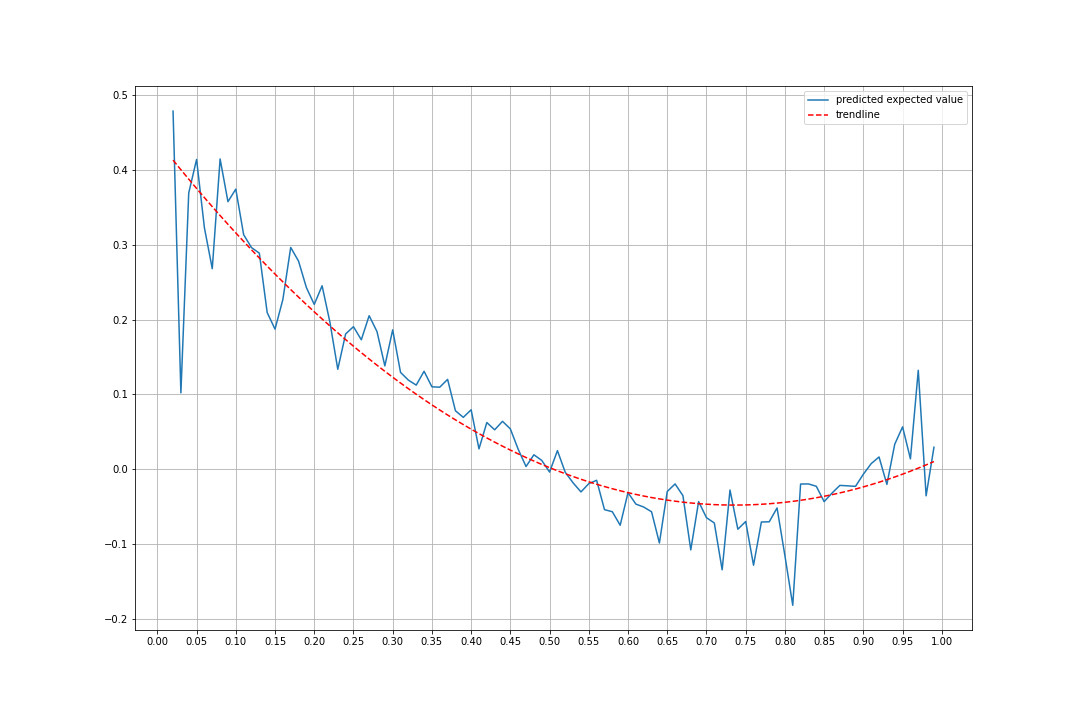
\includegraphics[width=\textwidth]{signatur_methode.png}
        {\footnotesize
        Für $H<1/2$ erkennen wir den ähnlichen Verlauf wie in Fig: (\ref{fig: becker_expec_vs_hurst}). Nur ist der maximaler Wert von der Signaturmethode bei 0.4 und der von Fig: (\ref{fig: becker_expec_vs_hurst}) bei 1.5 . Für $H=1/2$ liegt der Wert sowohl in der Signaturmethode als auch in Fig: (\ref{fig: becker_expec_vs_hurst}) bei 0, was auch mit der Theorie für das optimale Stoppen für Brownsche Bewegung übereinstimmt. Für $H>1/2$ erkennen wir den deutlichen Unterschied des Verlaufs beider Graphen. In der Signaturmethode liegen die Werte für den maximalen Erwartungswert bis $H<0.85$ in dem negativen Bereich, wohingegen der Wert in Fig: (\ref{fig: becker_expec_vs_hurst}) bis $H<1$ im positiven Bereich liegt und sogar eine monoton-wachsende Trend hat.
        \par}
      \end{figure}

      % Resultat aus der Hybridmethode
      \hfill\break
      Für die Hybridmethode eine Trainingsstichprobengröße von $M_{train}=3'000$ und eine Teststichprobengröße von $M_{test}=500$. Der Grund für die kleine Datenmenge ist der hohe Rechenaufwand. Das werden wir im nächsten Abschnitt genauer diskutieren. Für die Erstellung des Graphen berechnen wir für $H \in \{0.05,0.1,0.15,\ldots,0.90,0.95\}$ jeweils den Wert für $\mathbb{E}[Y_{\tau}]$. Für die Adam Methode haben wir $r = 0.01, \beta_1 = 0.9, \beta_2 = 0.999$ und $\varepsilon = 10^{-8}$ gewählt. Eine Darstellung des Graphen findet man in Fig: (\ref{hybrid_method}).
      \begin{figure}[H]\label{hybrid_method}
        \caption[hybrid_method]{Hybridmethode}
        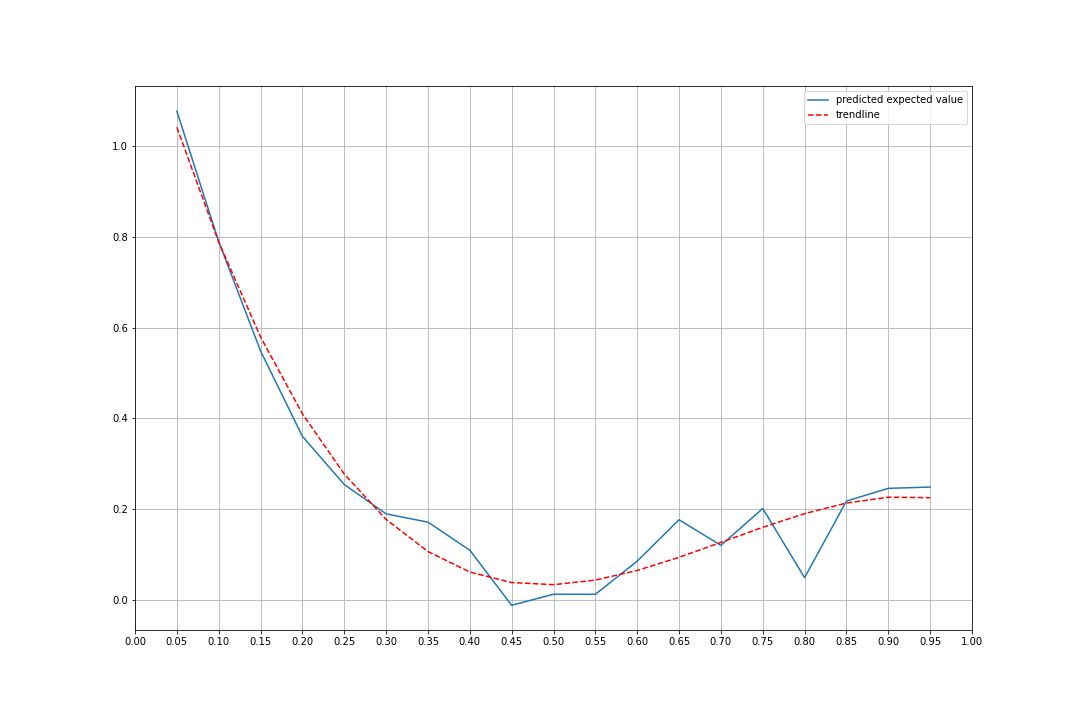
\includegraphics[width=\textwidth]{hybrid_methode.png}
        {\footnotesize
        Hier erkennt man einen deutlich besseren Verlauf mit dem maximalen Wert $1.12$ für $\underset{\tau \in \mathcal{T}}{sup} \ \mathbb{E}[Y_{\tau}]$ in $H=0.05$. Auch der Verlauf für $H>1/2$ kommt dem vom Benchmark nah. In dem Punkt $H=1/2$ ist aber der Wert nicht bei 0.
        \par}
      \end{figure}
      \newpage

      \subsection{Diskussionen}
      Dadurch, dass die Berechnung der optimalen Lösung in der Signaturmethode durch das Lösen eines linearen Gleichungssystems mithilfe der Methode der kleinsten Quadrate erfolgt, haben wir die Möglichkeit, die Lösungstheorie aus der linearen Algebra anzuwenden, d.h. wir können die Parameter wie das Niveau der Signaturen $N$ und die Anzahl an Daten $M$ so anpassen, damit wir für die Datenmatrix der Signaturen den vollen Rang bekommen und somit die Eindeutigkeit der Lösung erhalten. Jedoch benötigen wir für die Analyse der Lösungsqualität von der Signaturmethode weitere Forschungsanalysen und theoretische Beweise. Darüber hinaus besitzt die optimale Lösung $\tau_{l^*}$ eine recht einfache Struktur dank der Einfachheit der Signaturmethode im Vergleich zu der Hybridmethode, da diese durch das Bestimmen einer Hyperebene $\langle l,\hat{\mathbb{X}}^{\leq N}_{0,t}\rangle = 1$ berechnet wird und damit die schöne Eigenschaft der Linearität besitzt. Zu guter Letzt ist der Trainingsaufwand von der Signaturmethode aufgrund der einfachen Struktur und Linearität wesentlich geringer als die von der Hybridmethode. Das ist ein klarer Vorteil, wenn wir mit größeren Datenmengen arbeiten. (siehe Vergleich der Rechenzeit Tabelle: \ref{tbl:vergleich_rechenzeit})
      \hfill\break
      Der fatale Nachteil der Signaturmethode ist die Präzision. Wir vermuten, dass es durch das Bestimmen der optimalen Lösung $l$ geschieht. Wir betrachten in der Signaturmethode für die Berechnung von $l$ alle Trainingsdaten und alle Zeitpunkte. Dadurch hat man ein globales $l$ für alle Zeitpunkte bestimmt und verliert dabei die lokale Präzision für $l$. Die dadurch berechnete Lösung weist eine große Abweichung von dem Benchmark Fig: (\ref{fig: becker_expec_vs_hurst}) auf. Wir sehen, dass unser maximaler Wert für den Erwartungswert bei $0.48$ für $H=0.02$ und der von Fig: (\ref{fig: becker_expec_vs_hurst}) bei $1.51$ für $H=0.01$. Wir sehen auch in der Trendlinie, dass zwar der Trend für
      $H\leq1/2$ noch im Einklang mit dem Trend von Fig: (\ref{fig: becker_expec_vs_hurst}) ist, jedoch einen ganz anderen für $H>1/2$ aufweist. Zwar haben beide Graphen in $H=1/2$ den Wert $0$. Doch in der Signaturmethode erreichen wir den Tiefpunkt erst bei $H=0.74$ gemäß der Trendline oder $H=0.81$ gemäß des Graphen, wohingegen in $H=1/2$ der Benchmark seinen Tiefpunkt bereits erreicht hat.
      \begin{table}[H]
        \caption{Vergleich der durchschnittlichen Rechenzeit (gerundet)}
        \centering
        \begin{tabular}{rrr}
          \midrule
          M & Signaturmethode (Sekunden) & Hybridmethode (Sekunden) \\
          \toprule
          1000 & 8.99 & 9872.26 \\
          5000 & 15.64 & 34883.11 \\
          10000 & 48.32 & 78413.32 \\
          \midrule
        \end{tabular}
        \label{tbl:vergleich_rechenzeit}
      \end{table}

      \hfill\break
      Einen klaren Nachteil hat auch die Hybridmethode. Die Trainingszeit ist vergleichweise sehr lang. Im Gegensatz zu der Signaturmethode, die den gesamten untersuchten Prozess vom Zeitpunkt $0$ bis zu $T$ betrachtet, berechnet die Hybridmethode den Prozess von $0$ bis zu den einzelnen diskreten Zeitpunkten $t_k \in (0,T)$ separat.
      \hfill\break
      Das führt dazu, dass der Rechenaufwand für die Monte-Carlo Approximation für den Erwartungswert durch die Anzahl der Schrittweite vervielfacht hat. Außerdem ist das Konvergenzverhalten von der Adam zwar besser als die konventionelle Gradient Descent Methode. Jedoch konvergiert Adam in manchen Fällen erst nach 50 Iterationen. Die genaue Messdaten für die Rechenzeit mit verschiedenen Datengrößen findet man in der Tabelle (\ref{tbl:vergleich_rechenzeit}).
      \hfill\break
      Jedoch hat die Hybridmethode einen klaren Vorteil gegenüber der Signaturmethode, nämlich die Präzision. Durch die Zerlegung der Stoppzeit in die lokalen Stoppentscheidungen in den einzelnen diskreten Zeitpunkten ermöglicht die Hybridmethode ein vergleichbares Resultat zu dem Benchmark. Wir sehen, dass der maximaler Wert für den Erwartungswert bei $1.1$ für $H=0.05$ liegt, wohin gegen der maximaler Wert vom Benchmark bei $1.51$ für $H=0.01$ ist. Außerdem können wir einen vergleichbaren Verlauf des Erwartungswerts bezüglich des Hurstparameters erkennen: den steilen Abstieg für $H<1/2$ und den milden Anstieg für $H>1/2$. Für $H=1/2$ liegt der Erwartungswert zwar nicht bei 0 und es existiert kleine Abweichungen bei der Messung. Jedoch sollten wir berücksichtigen, dass wir für unsere Messung wegen des hohen Rechenaufwands und der Einschränkung des Hardwares eine sehr kleine Stichprobengröße gewählt haben ($M_{train}=3000$) und die Anzahl an Testdaten ebenfalls ($M_{test} = 500$). Zusätzlich ist es zu erwähnen, dass die Hybridmethode durch die Kombination des Signaturansatzes und des Ansatzes für das tiefneuronale Netzwerk innovativ ist und eine neue Idee für die künftige Forschung liefern kann.
      \hfill\break
      Zusätzlich haben wir die relative Häufigkeit der berechneten Stoppzeit von beider Methoden für die Hurstparameter $H = \{0.05,0.1,0.15,\ldots,0.9,0.95\}$ gemessen. Als Beispiel betrachten wir die Messung für $H=0.8$ Fig: (\ref{verteilung_vergleich_0_8}). Weitere Graphiken findet man in Appendix \ref{appendix:plots}.
      \hfill\break
      Wir erkennen, dass die Signaturmethode dazu tendiert, direkt nach dem Starten des Prozesses zu stoppen, wohingegen die Hybridmethode dazu geneigt ist, zum Endzeitpunkt zu stoppen. Ein möglicher Grund für das Verhalten von der Hybridmethode kann ihre Konzeption sein. Wir initialisieren zum Zeitpunkt $T$ die lokale Stoppentscheidung mit $1$ und iterieren rückwärts, um die Stoppentscheidungen in den vorigen Zeitpunkten zu berechnen. Dabei haben wir für die Stoppentscheidung die Regel
      $f_n^{l_n^*} := \mathds{1}_{ \{ \langle l_n^*, \hat{\mathbb{X}}^{< \infty}_{0,t_n}  \rangle \geq 1 \} }$ definiert. Das bedeutet, $f_n^{l_n^*}=1$ gilt genau dann, wenn die Bedingung $\langle l_n^*, \hat{\mathbb{X}}^{< \infty}_{0,t_n}  \rangle \geq 1$ erfüllt ist. In den Messungen ist es der Fall eingetreten, dass diese Bedingung für die meisten Pfade
      $\langle l_n^*, \hat{\mathbb{X}}^{< \infty}_{0,t_n}  \rangle \geq 1$ nicht erfüllt ist und somit $f_n^{l_n^*}=0$ für alle $n<T$. Damit stoppt die durch die Hybridmethode bestimmte Stoppzeit die Testprozesse bei $T=1$.
      \begin{figure}[H]
        \caption{Vergleich der relativen Häufigkeit der Stoppzeiten für FBM in beider Methoden mit $H=0.8$}
        \subfigure[Signaturmethode]{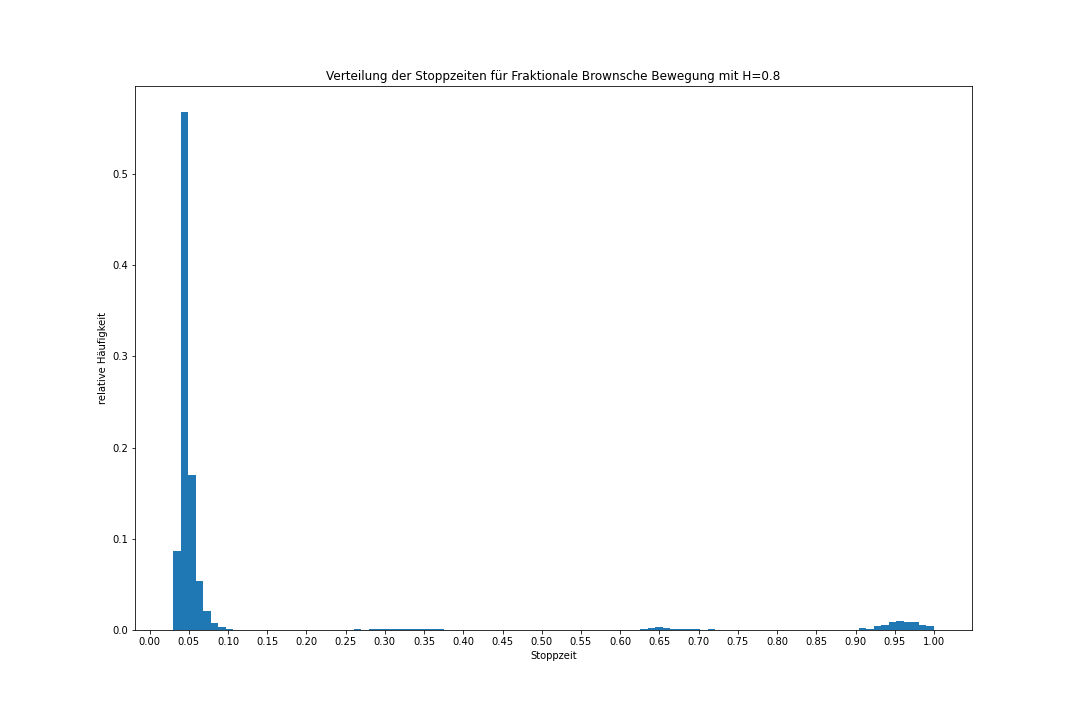
\includegraphics[width=.49\textwidth]{signatur/histogram_0_8.png}}
        \subfigure[Hybridmethode]{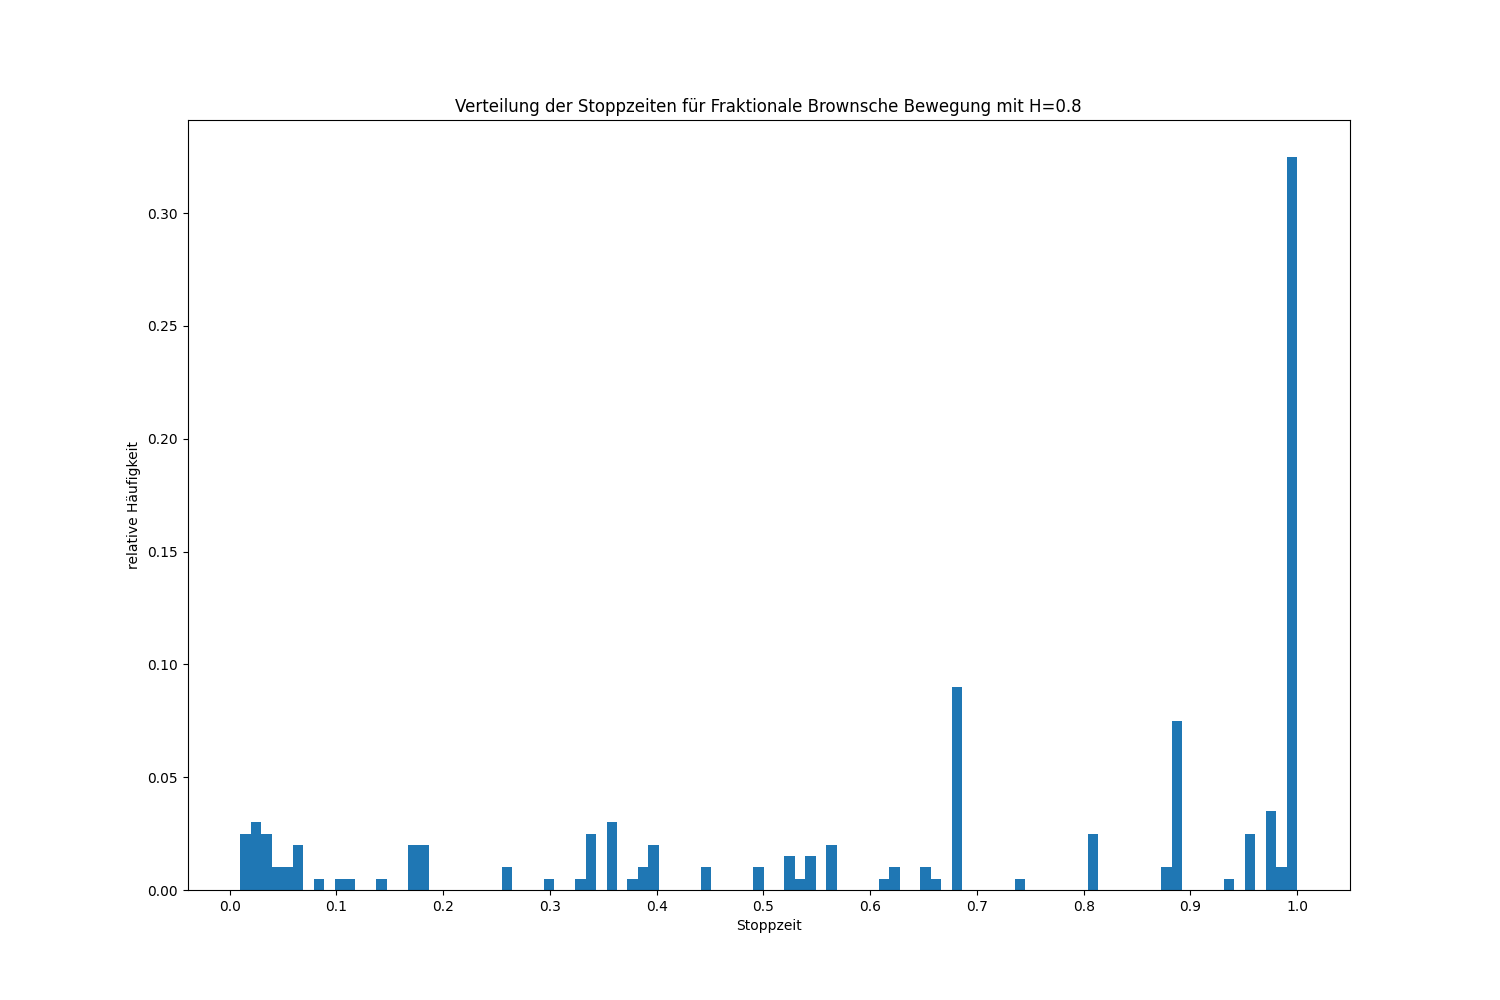
\includegraphics[width=.49\textwidth]{hybrid/histogram_0_8.png}}
        \label{verteilung_vergleich_0_8}
      \end{figure}
      \hfill\break
      Zusammengefasst halten wir fest, dass die Signaturmethode durch ihre Linearität sehr kurze Rechenzeit hat und dadurch für die Verarbeitung von großen Mengen an Daten oder auch multi-dimensionalen Daten sehr gut geeignet ist. Jedoch wird sie erst Anwendung in der Praxis finden, wenn die Qualität der Approximation für die optimale Stoppzeit sich verbessert. Es gibt bislang keine wissenschaftliche Forschungsergebnisse für die Analyse der Qualität bezüglich des optimalen Stoppens mit der Signatur. Das bietet daher eine Grundlage für weitere Forschungsideen.
      \hfill\break
      Eine Möglichkeit zur Verbesserung der Optimierungsgeschwindigkeit oder auch -qualität in der Hybridmethode ist ein Vergleich der Gradientenverfahren angewandt auf unser Beispiel. Wir haben in dieser Arbeit Adam gewählt, da diese in jedem Schritt die Schätzung für den ersten und den zweiten Moment der Gradienten zur Rechnung gezogen hat und sich für die stochastische Optimierung in der Praxis als effizient herausgestellt hat. Als die Approximation für die Stoppentscheidung in der Hybridmethode haben wir die angepasste logistische Funktion (oder auch Sigmoidfunktion) $F(X)=\Phi(\langle l, X \rangle)$ ausgewählt. Das Phänomen verschwindente Gradienten (Vanishing Gradient) ist bei uns eingetreten. Das heißt, die Gradienten sind ab einem bestimmten Iterationsschritt dünnbesetzt und die gradientenbasierte Methode konvergiert ab dem Zeitpunkt sehr langsam. Aus der Praxis in der Anwendung von tief neuronalen Netzwerken hat sich herausgestellt, dass die logistische Regression das Phänomen verursacht und man entweder eine andere Aktivierungsfunktion oder eine andere Optimierungsmethode wählt. Es sollte daher in die Richtung geforscht werden, welche Optimierungsmethode für die Hybridmethode am besten geeignet ist. Kandidaten dafür sind zum Beispiel die ReLU Funktion oder auch die RelTan Funktion \cite{wang_reltanh_2019}.
      \hfill\break
      Zwar gibt es die Konvergenzanalyse von \cite{becker_deep_2019} für DNN. Aber die Konvergenz der Hybridmethode ist nicht untersucht. Desweiteren ist die Forschung über den Zusammenhang zwischen dem Niveau der Signatur und der Qualität des optimalen Stoppens erwünscht. Es ist intuitiv, dass je höher das Niveau ist, umso größer ist der Informationsgehalt von dem Pfad. Aber wir sollten bedenken, je höher das Niveau ist, umso mehr Rechenaufwand benötigt die Methode für die Bestimmung der optimalen Stoppzeit. Die Idee ist also, durch numerische Experimente das optimale Niveau $N^*$ zu finden, das eine gute Qualität für das Lösen vom optimalen Stoppen ohne enormen Rechenaufwand liefert.
      \hfill\break
      Da Rough Path eine mächtige Methode zur Untersuchung von stochastischen Prozessen ist und über die Einschränkungen wie die Markoveigenschaft oder auch die Martingaleigenschaft hinausgeht, kann man in die Richtung der Finanzmathematik untersuchen, wie die Qualität der beiden Methoden bei Optionsbepreisung ist. Ein Beispiel mit der amerikanische Put Option hat man bereits in \cite{bayer_optimal_2020} mit der Deep Signatur Methode untersucht.

      \newpage

    \section{Fazit}
      % Optimal Stopping mit Rough Path
      In dieser Arbeit haben wir zwei Methoden für das optimale Stoppen mit Rough Path untersucht. Im Vergleich zu den konventionellen Ansätzen wie der Martingalansatz oder der Markovansatz verwendet man dabei die Signatur eines Rough Paths.
      \hfill\break
      Im Kapitel \ref{chapter: opt_stop_with_rough_path} haben wir die Rough Path Theorie mithilfe von \cite{bayer_optimal_2020} eingeführt. Ein Rough Path, genauer, ein geometrischer p-Rough Path ist eine Abbildung $\mathbb{X}: [0,T] \mapsto G^{\lfloor p \rfloor}(V)$ gestartet mit 1, von endlichen p-Variationen und ist der Grenzwert von der Folge der durch $\lfloor p \rfloor$ abgeschnittenen Signatur von stückweise glatten Pfaden. Die Motivation dafür war, dass man mit den iterierten Integralen in einem Rough Path mehr Information über den zugrundeliegenden Pfad gewinnen kann. Mit dieser Idee hat man das Polynom $l$ im Bezug zu der Signatur eingebracht, welches durch die Charakterisierung der Elemente aus dem Raum der Wörter entstanden ist. Damit konnte man die Stopp
      Police $\theta \in \mathcal{T}_{sig}$ derfinieren, für diese das folgende gilt:
      \begin{align*}
        \mathds{1}_{\tau(\omega)\leq t}= \theta(\hat{\mathbb{X}}\lvert_{[0,t]}) = \langle l, \hat{\mathbb{X}}_{0,t}^{< \infty} \rangle.
      \end{align*}
      Mit dem Lemma (\ref{lemma: bayer_st_theta}) und der Definition (\ref{def: stopp_police}) kann man für jede Stoppzeit $\tau \in \S$ ein $l \in T((\mathbb{R}^{1+d})^*)$ finden. Mit dieser Erkenntnis wurde die Signatur Stoppzeit
      $\tau_l = inf \{t \in [0,T] : \langle l, \hat{\mathbb{X}}_{0,t}^{< \infty} \rangle \geq 1 \}$ über die randomisierte Signatur Stoppzeit hergeleitet und die Kernidee für unsere beiden Methoden wurde gebildet.
      \hfill\break
      Im Kapitel 3 haben wir die zwei Methode zur Lösung vom optimalen Stoppen mit Rough Path präsentiert. Die Signaturmethode stammt direkt aus dem Theorem (\ref{theorem: main_result}) und es ist einem klar, dass zur Bestimmung der optimalen Signatur Stoppzeit wir das optimale $l$ bestimmen müssen. Aus diesem Grund haben wir mithilfe der Hyperebene $\langle l, \hat{\mathbb{X}}_{0,t}^{< \infty} \rangle = 1$ ein lineares Gleichungssystem aufgestellt und das mit der Methode der kleinsten Quadrate gelöst.
      \hfill\break
      Im Gegensatz zu der Einfachheit der Signaturmethode orientieren wir uns für die Hybridmethode an dem komplexen Ansatz von \cite{becker_deep_2019}. Der Kandidat für die optimale Stopzeit ist gegeben durch:
      \begin{align*}
        \tau^* = \sum_{n=1}^K t_nf_n^{l_n}(\hat{\mathbb{X}}^{\leq N})\prod_{j=0}^{n-1}(1-f_j^{l_j}(\hat{\mathbb{X}}^{\leq N})).
      \end{align*}
      Wir benutzen für die Stoppentscheidungen $f_n^l$ die Approximation
      \begin{align*}
        F_n^l(\hat{\mathbb{X}}_{0,t}^{\leq N}) = \psi(\langle l, \hat{\mathbb{X}}_{0,t}^{\leq N} \rangle - 1)
      \end{align*}
      anstatt ein tief neuronales Netzwerk wie in \cite{becker_deep_2019}.
      \hfill\break
      Die numerische Resultate aus \cite{becker_deep_2019} dienen als der Benchmark für unsere Methode. Verglichen werden die berechnete Werte für $\mathbb{E}[Y_{\tau^* \wedge T}]$ mit den jeweiligen bestimmten optimalen Stoppzeiten $\tau^*$. Die Resultate aus den numerischen Experimenten zeigen, dass qualitativ die Hybridmethode deutlich überragener ist. Aber die Laufzeitperformence ist im Vergleich zu der Signaturmethode deutlich schlechter. Jedoch schränkt unser Hardware uns bei der Performance stark ein, was definitiv einen Einfluss auf die Laufzeit hat.
      \hfill\break
      Zwar ist die Optimalität der Stoppzeit in der Hybridmethode durch Lemma (\ref{lemma: bayer_st_theta}) gewährleistet. Jedoch haben wir die Konvergenzanalyse für das Funktional in (\ref{eqn: l_n}) in dieser Arbeit nicht diskutiert. Im Hinblick darauf kann es sinnvoll sein, theoretische Beweise dafür zu erforschen. Weiterführende Forschung könnte die Verbesserung der Rechenzeit für die Hybridmethode aus einer neuen Perspektive betrachten. Wenn der Rechenaufwand sich dadurch reduziert hat, könnte die zukünftige Forschung an weitere Anwendungsfälle knüpfen, indem man z.B. diese Methode für die Bepreisung von Optionen wie die American Put Option oder die Bermudan-Max-Call Option einsetzt.
    \printbibliography

    \newpage

    \appendix

    \section{Appendix}

      \subsection{Fraktionale Brownsche Bewegung}\label{appendix:fbm}
      In diesem Abschnitt gehen wir auf das Objekt \textit{fraktionale Brownsche Bewegung}(kurz FBM) ein. Dabei nennen wir nur die Definitionen und Theoreme, die für diese Arbeit wichtig sind. Für interessierte Leser empfehlen wir das Paper \cite{shevchenko_fractional_2014} oder auch die Standardliteraturen für Stochastische Prozesse.
      Die fraktionale Brownsche Bewegung gehört zu der Klasse der Gaußprozessen. Diese Klasse wurde im Jahr 1940 von Kolmogorov mit dem Rahmen des Hilbertraums eingeführt. Die Intuition für diese Klasse von stochastischen Prozessen ist die Beschreibung der fraktionale Bewegungsdynamiken, z.B. jährlicher Wasserabfluss des Nilflußes oder Aktienkurs, wo diese Klasse ihre meiste Anwendung findet. Man kann FBM bezüglich dem Hurstparameter $H$ grob in drei Familien unterteilen, nämlich in $0<H<1/2$, $H=1/2$ und $1/2<H<1$. Eine allgemeine Definition sehen wir wie folgt:
      \begin{definition}
        Sei $(B_t^H)_{t \geq 0}$ ein Gaußprozess. Eine fraktionale Brownsche Bewegung ist ein zentrierter Gaußprozess mit der Kovarianzfunktion:
        \begin{align*}
          \mathbb{E}[B_t^HB_s^H]=\frac{1}{2}(t^{2H}+s^{2H}-{\lvert t-s \rvert}^{2H}).
        \end{align*}
        Der Prozess hat den Parameter $H \in (0,1) $, welcher den Hurst Parameter oder auch Hurst Index genannt wird.
      \end{definition}
      \begin{bemerkung*}
        \textup{
        Ein Gaußprozess $(X_t)_{t \geq 0}$ ist ein stochastischer Prozess mit Komponenten, die jeweils normalverteilt sind und heißt zentriert, falls $\mathbb{E}[X_t]=0, \ \forall t \in [0,T]$
        }
      \end{bemerkung*}
      Im Folgenden werden wir die wichtigen Eigenschaften der FBM präsentieren. Um die Verteilung eines Gauß Prozesses zu untersuchen, ist es ausreichend, deren Erwartungswerte und Kovarianzen zu untersuchen. Für jede H ist die Verteilung von $B^H$ eindeutig durch obige Definition bestimmt. Für $H = 1/2$ ist $B^H$ eine Brownsche Bewegung. Es gibt drei wesentliche Merkmale für FBM:
      \begin{itemize}
        \item [1] \textbf{Stationäre Inkremente} Für $t \geq 0$ betrachten wir den Prozess $Y_t = B_{t+s}^H - B_s^H$. Dann gilt $\mathbb{E}[Y_tY_s] = \mathbb{E}[B_t^HB_s^H]$, d.h. $Y$ hat die gleiche Kovarianz wie $B^H$ und somit auch die gleiche Verteilung.
        \item [2] \textbf{Selbstähnlichkeit}(H-Selbstähnlichkeit) Sei $a > 0 $ und $Z_t = B_{at}^H, \ t\geq 0$. Dann hat $Z$ die gleiche Kovarianz und die gleiche Verteilung wie $a^HB^H$, d.h. der Prozess ist invariant gegenüber einer Skalierung der Zeit.
        \item [3] \textbf{Abhängigkeit von Inkrementen} Sei $s_1 < t_1 < s_2 < t_2 $ mit $[s_1,t1]$ und $[s_2,t_2]$ disjunkt. Dann kann man die linke Seite von
        \begin{align*}
          & \mathbb{E}[(B_{t_1}^H - B_{s_1}^H)(B_{t_2}^H-B_{s_2}^H)] \\
          & =\frac{1}{2}(\lvert t_1-s_2 \rvert^{2H} + \lvert t_2-s_1 \rvert^{2H} - \lvert t_2-t_1 \rvert^{2H} + \lvert s_2-s_1 \rvert^{2H})
        \end{align*}
        schreiben als $((f(a_1)-f(a_2))-(f(b_1)-f(b_2))) / 2$, wobei $a_1 = t_2-s_1, \ a_2 = t_2 - t_1, \ b_1 = s_2 - s_1, \ b_2 = s_2 - t_1, \ f(x)=x^{2H}$. Wir können durch die Konvexität von $f$ folgendes beobachten:
        \begin{align*}
          & \mathbb{E}[(B_{t_1}^H - B_{s_1}^H)(B_{t_2}^H-B_{s_2}^H)] < 0 \ for \ H \in (0,1/2) \\
          & \mathbb{E}[(B_{t_1}^H - B_{s_1}^H)(B_{t_2}^H-B_{s_2}^H)] > 0 \ for \ H \in (1/2,1).
        \end{align*}
        Für $H \in (0,1/2)$ hat die FBM die Eigenschaft Konterpersistenz, d.h. wenn der Prozess in der Vergangenheit ein monoton wachsendes Wachstum aufweist, ist es wahrscheinlicher, dass der Prozess in der Zukunft monoton fällt und vice versa. Dagegen ist der Prozess für $H \in (1/2,1)$ persistenz, d.h. die monotone Eigenschaft bleibt auf dem gesamten Zeithorizont unverändert. Für solche $H$ hat die FBM die Eigenschaft des Long-Memory.
      \end{itemize}
      % \textcolor{red}{Stetigkeit von FBM:}
      % Wie bei jedem stochastischen Prozess interessieren wir auch für die Stetigkeit der FBM. Es gibt viele Möglichkeiten, die Stetigkeit nachzuweisen. In dieser Arbeit werden wir das \textit{Kolmogorov-Chentsov Theorem} vorstellen. Nichtsdestotrotz basieren alle Möglichkeiten für den Nachweis der Stetigkeit auf der selben Formel:
      % \begin{align*}
      %   \mathbb{E}[(B_t^H - B_s^H)^2] = \lvert t-s \rvert^{2H}
      % \end{align*}
      % für das \textcolor{red}{Variogram} der FBM.
      % \begin{theorem-non}[Kolmogorov-Chentsov Stetigkeitstheorem]
      %   Sei $(X_t)_{t \geq 0}$ ein stochastischer Prozess. Angenommen es existieren $K>0, p>0, \beta > 0 $, so dass für alle $t \geq 0, s\geq 0$ gilt:
      %   \begin{align*}
      %     \mathbb{E}[\lvert X_t - X_s\rvert^p] \leq K \lvert t -s \rvert^{1+\beta}.
      %   \end{align*}
      %   Dann hat der Prozess eine stetige Modifikation, d.h. es gibt einen Prozess $\tilde{X}_t$ mit $\tilde{X} \in \mathcal{C}([0,\infty)$ und für alle $t\geq 0$ gilt $\mathbb{P}(X_t = \tilde{X}_t)=1$. Ferner ist für alle $\gamma \in (0,\frac{\beta}{p})$ und für $T>0$ ist der Prozess $\tilde{X}$ $\gamma$-Hölder stetig auf $[0,T]$:
      %   \begin{align*}
      %     \underset{0\leq s < t \leq T}{sup} \ \frac{\lvert \tilde{X}_t - \tilde{X}_s\rvert}{(t-s)^{\gamma}} < \infty.
      %   \end{align*}
      % \end{theorem-non}
      % \begin{corollary-non}
      %   Die fraktionale Brownsche Bewegung $B^H$ hat stetige Modifikation. Ferner ist diese Modifikation $\gamma$-Hölder stetig auf jedem endlichen Zeitintervall für alle $\gamma \in (0,H)$.
      % \end{corollary-non}
      % \begin{beweis-non}
      %   \textup{
      %   Da $B_t^H - B_s^H$ ein zentrierter Gaußprozess mit der Varianz $\lvert t - s \rvert^H$ ist, gilt $\mathbb{E}[\lvert B_t^H - B_s^H \rvert]=K_p\lvert t - s \rvert^{pH}$. Wähle $p > 1/H$, dann erhalten wir die Existenz der stetigen Modifikation mit Kolmogorov-Chentsov Stetigkeitstheorem. Die Bedingung für die Hölder Stetigkeit von der Modifikation mit $\gamma \in (0,H-1/p)$ auch erfüllt, wenn wir $p$ hinreichend groß wählen.
      %   }
      % \end{beweis-non}
      % Für weitere Methoden verweisen wir auf \cite{shevchenko_fractional_2014}.
      \begin{bemerkung*}
        \textup{
        Abhängig von $H \in (0,1/2)$ bzw. $H \in (1/2,1)$ sind die Inkremente von der FBM negativ bzw. positiv korreliert \cite{grimmett2020probability}. Außerdem wachsen die Korrelation und die Persistenz der FBM mit $H$. Für $H=1$ wird die FBM zu einer linearen Funktion: $B_t^1=\xi t$, wobei $\xi$ ein Standard Gaußprozess ist.
        }
      \end{bemerkung*}
      % \textcolor{red}{Integralrepräsentation von FBM (ist das denn überhaupt noch notwendig???) JA: das zeigt die Existenz der FBM}: Das Konzept für die integrale Repräsentation der FBM ist vergleichbar mit der klassischen Ito Repräsentation für Martingale. Sei also $(W_t)_{t\geq 0}$ ein reellwertiger Wiener Prozess, so dass $(W_t)_{t\geq0}$ und $(W_{-t})_{t\geq 0}$ unabhängige Standard Wiener Prozesse auf $[0,\infty )$ sind. Für Funktionen $f \in \mathcal{L}^2(\mathbb{R})$ ist das Integral $I(f) = \int_{\mathbb{R}}f(x)dW(x)$ bzgl. $W$ durch maßtheoretische Induktion von einfachen Indikatorfunktionen bis hinzu
      % $\mathcal{L}^2$ Funktionen mit der Ito Isometrie konstruiert.\cite{Kapitel 25, Wahrscheinlichkeitstheorie, Achim Klemke}
      %
      % Für die Existenz der FBM betrachten wir die Repräsentation folgender Form:
      % \begin{align*}
      %   B^H_t = I(k_t)=\int_{\mathbb{R}}k_t(x)dW(x),
      % \end{align*}
      % \begin{bemerkung*}[Mandelbrot-van Ness Repräsentation]
      %   \textup{
      %   Für $H \in (0,1)$ definieren wir:
      %   \begin{align*}
      %     k_H^{MA}(x)=K_H^{MA}((t-x)_t^{H-1/2}\mathds{1}_{(-\infty,0)(x)-(-x)^{H-1/2}}),
      %   \end{align*}
      %   wobei $K_H^{MA} = (\frac{1}{2H} + \int_0^\infty((x+1)^{H-1/2}-x^{H-1/2})^2dx)^{-1/2} = \frac{(\Gamma(2H+1)sin \pi H)^{1/2}}{\Gamma (H+1/2)}$. Dann ist der Prozess $X_t = I(k_t^{MA})$ eine fBm mit dem Hurst Parameter H und es gilt $k_t^{MA} \in L^2(\mathbb{R})$.
      %   \begin{itemize}
      %     \item das ist eine Integral Repräsentation mit Moving Average
      %     \item es gibt noch andere wie z.B. blablabla. detailierte Informationen findet man in \cite{Fractional Brownian Motion in a Nutshell}
      %   \end{itemize}
      %   }
      % \end{bemerkung*}
      % \hfill\break
      % \textcolor{red}{wofür habe ich das nochmals gebraucht?} Für die Analyse der Resultate aus unserem Experiment möchten wir \textit{das Gesetz der iterierten Logarithmus} vorstellen. Wir starten mit der Brownschen Bewegung. Sei $(B_t)_{t\geq 0}$ eine Brownsche Bewegung. Das \textit{Blumenthal'sche 0-1 Gesetz} für Brownsche Bewegung besagt
      % \begin{itemize}
      %   \item wir starten mit Brownsche Bewegung
      %   \item Motivation: Blumenthal'schen 0-1 Gesetz für BM
      %   \begin{align*}
      %     \underset{t \rightarrow 0 }{limsup} \frac{B_t}{\sqrt{t}}= \infty f.s.
      %   \end{align*}
      %   \item mit $tB_{1/t}$ ist eine BM gilt dann:
      %   \begin{align*}
      %     \underset{t \rightarrow \infty }{limsup} \frac{B_t}{\sqrt{t}}= \infty
      %   \end{align*}
      %   \item Ziel: ersetze $\sqrt{t}$ durch eine Funktion, so das Limes Superior endlich und nicht trivial ist.
      %   \item Erweiterung auf fBm...
      % \end{itemize}
      % \begin{theorem}[Gesetz der iterierten Logarithmus]
      %   Sei $B_t$ eine Brownsche Bewegung. Dann gilt:
      %   \begin{align*}
      %     \underset{t \rightarrow \infty}{limsup} \frac{B_t}{\sqrt{2t \ log(log(t))}} = 1, \ f.s.
      %   \end{align*}
      % \end{theorem}
      %
      % \hfill\break
      % hier kommt der letzter Abschnitt. Folgende Punkte sollten erläutert werden:
      % \begin{itemize}
      %   \item financial modelling with fBm
      %   \item pathwise integration with fbm
      %   \item fbm in physics
      %   \item other important results for fbm
      % \end{itemize}


      \newpage

      \subsection{Monte Carlo Simulation}\label{appendix:mc-methode}
      Wir präsentieren in diesem Abschnitt die für diese Arbeit notwendige Kenntnisse über Monte Carlo Simulation. Für die weitere Literaturen verweisen wir auf \cite{kalos_monte_2008, shapiro_stochastic_2000}. Das erste Buch gibt einem das Grundverständnis für die Monte Carlo Methode und in dem zweiten Buch wird vorwiegend über die Anwendung der Monte Carlo Simulation in der stochastischen Programmierung vorgestellt.
      \hfill\break
      Simulation findet in vielen Industriebereichen ihre Anwendung wie z.B. Automobilie, Flugzeugbau oder auch Filmindustrie. Der Unterschied von Monte-Carlo (MC) Simulation zu den traditionellen Simulationen ist der, dass die Parameter in dem simulierten Model als eine Zufallsvariable behandelt wird anstatt als einen deterministischen Wert. Die \textit{Monte Carlo} Simulation hat seine erste Anwendung in einer Klasse von mathematischen Methoden gefunden, die man für die Entwicklung der Nuklearwaffen in Los Alamos im Jahr 1940 während des zweiten Weltkriegs erarbeitet hat. Der Name wurde nach der berühmten Stadt in Monaco benannt.
      \hfill\break
      Die Idee von MC Simulation beruht auf das Gesetz der großen Zahlen und besteht darin, wiederholt Stichproben von der Verteilung der Zufallsvariable zu generieren, sodass man am Ende eine Menge von möglichen Realisierungen der Zufallsvariable hat. Das zulösende Problem bzw. Funktional ist durch den empirisch bestimmten Wert approximiert, d.h. der Erwartungswert einer Zufallsvariable $\mathbb{E}[X]$ wird durch den Durchschnitt $1/N \sum_{i=1}^N X_i$ approximiert, wobei $X_i$ die i-te Stichprobe von der Zufallsvariable $X$ ist. Je größer die generierte Menge ist, umso genauer wird die Simulation sein. Es wird dabei vorausgesetzt, das man die Verteilung der Zufallsvariable a priori kennt, z.B. eine Normalverteilung mit dem Erwartungswert $\mu$ und der Varianz $\sigma^2$.
      \hfill\break
      Für unsere Arbeit ist die numerische Approximation des Erwarungswerts wichtig. Wir konzentrieren uns auf die stochastische Programmierung mit MC Methode und haben das folgende Optimierungsproblem als Ausgangspunkt:
      \begin{align}\label{mc:opt-problem}
        \underset{\tau \in \mathcal{T}}{max} \ \mathbb{E}[g(\tau,X_{\tau})].
      \end{align}
      Da wir in dem Problem eine nicht-deterministische Größe $X_{\tau}$ haben, können wir den Erwartungswert nicht deterministisch bestimmen ($\tau$ ist hier auch eine Zufallsgröße). Um die Lösung für (\ref{mc:opt-problem}) zubestimmen, approximieren wir $\mathbb{E}[g(\tau,X_{\tau})]$ durch den Schätzer:
      \begin{align}\label{mc:opt-problem-approx}
        \frac{1}{N}\sum_{i=1}^N g(\tau,X_{\tau}^i),
      \end{align}
      wobei $X_{\tau}^1,\ldots,X_{\tau}^N$ die Stichproben von $X$ sind.
      Eine solche Art von Approximation nennen wir \textit{Sample Average Approximation}. Falls für alle $i$ gilt, dass $ \mathbb{E}[g(\tau,X_{\tau}^i)] = g(\tau,X_{\tau})$ und $g$ linear in $X$ ist, dann haben wir:
      \begin{align*}
        \mathbb{E}[\frac{1}{N}\sum_{i=1}^N g(\tau,X_{\tau}^i)] = \frac{1}{N}\sum_{i=1}^N \mathbb{E}[g(\tau,X_{\tau}^i)] = g(\tau,X_{\tau})
      \end{align*}
      d.h. der Schätzer ist erwartungstreu. Aus der Statistik wissen wir, dass die erwartungstreue Schätzer keinen systematsichen Fehler haben.
      \hfill\break
      In der Hybridmethode betrachten wir das Optimierungsproblem:
      \begin{align*}
        \underset{l \in \mathcal{T}((\mathbb{R}^{1+d})^*)}{argmax} \ \mathbb{E}[g(t_n, Y_{t_n})F_n^l(\hat{\mathbb{X}}^{< \infty})+g(\tau_{n+1},Y_{\tau_{n+1}})(1-F_n^l(\hat{\mathbb{X}}^{< \infty}))].
      \end{align*}
      Wir erinnern uns, dass wir für das Problem den Parameter $l$ in der Hyperebene bestimmen möchten. Der Schätzer für den Erwartungswert ist also:
      \begin{align*}
        \frac{1}{N} \sum_{k=1}^N g(t_n, Y^k_{t_n})F_n^l(\hat{\mathbb{X}}^{< \infty})+g(\tau_{n+1},Y^k_{\tau_{n+1}})(1-F_n^l(\hat{\mathbb{X}}^{< \infty}))
      \end{align*}
      mit Stichproben $Y^1,\ldots,Y^N$ von $Y$.
      \newpage

      \subsection{ADAM Methode}\label{appendix: adam method}

      Wir präsentieren in diesem Kapitel die Adam Methode von \cite{kingma_adam_2017}. Wir zeigen lediglich nur die Idee und die wichtige theoretische Resultate (insbesondere die Konvergenzanalyse) und verweisen auf \cite{kingma_adam_2017} für numerische Resultate.
      \hfill\break
      Die stochastischer Gradient basierte Optimierung ist ein wesentlicher Bestandteil in vielen Forschungsfeldern der Naturwissenschaft und des Ingenieurwesens. Viele Probleme können durch die Optimierung eines parametrisierbaren Zielfunktional dargestellt werden, in dem man es über die Parameter maximiert oder minimiert. Falls das Funktional differenzierbar bzgl. der Parameter ist, ist das intuitive effiziente Optimierungsverfahren zur Lösung solches Optimierungsproblems das \textit{Gradient Descent}. In der stochastischen Programmierung haben die Zielfunktionalen in den Parametern die Zufallsgrößen und man kann nicht wie im deterministischen Fall direkt über diese optimieren. Als Ausweg gibt es die Methode \textit{Stochastic Gradient Descent} (SGD). SGD zeigte sich als effiziente und effektive Optimierungsmethode, die in vielen Anwendungsfällen des maschinelles Lernens sowie in den neusten Fortschritten des Deep Learnings \cite{deng2013recent} eine wichtige Rolle spielt.
      \hfill\break
      Adam ist eine effiziente stochastische Optimierungsmethode, die nur Gradienten erster Ordnung benötigt. Das Verfahren berechnet in jedem Schritt adaptive Lernrate (auch Schrittweite) für alle Parameter aus Schätzungen des ersten und zweiten Moments der Gradienten. Der Name Adam kommt von \textit{adaptive moment estimation}. Diese Methode wurde entwickelt, um die Vorteile von AdaGrad \cite{duchi_adaptive_2011}, welche gut mit dünnbesetzten Gradienten funktioniert und RMSProp \cite{tieleman2012lecture}, welche in on-line und nicht stationärem Umfeld gut arbeitet, zu kombinieren. Einige Vorteile von Adam sind, dass die Schrittweiten nährungsweise durch den Schrittgrößen-Hyperparameter beschränkt sind, diese kein stationäres Zielfunktional erfordert und diese gut mit dünnbesetzten Gradienten funktioniert.
      \hfill\break
      Der Pseudo Code von Adam sieht wie folgt aus:
      \begin{algorithm}[H]\label{adam: algo}
        \caption{Pseudo Code für die Adam Methode. $g_t^2$ ist das elementenweise Quadrat $g_t \odot g_t$. Eine gute Voreinstellung für die numerische Experimente sind $\alpha = 0.001$, $\beta_1 = 0.9$, $\beta_2 = 0.999$ und $\varepsilon = 10^{-8}$. Alle Operationen auf Vektoren sind elementenweise. Mit $\beta_1^t$ und $\beta_2^t$ beschreiben wir $\beta_1$ und $\beta_2$ hoch $t$.}
        \begin{algorithmic}
          \Require $\alpha:$ Stepsize
          \Require $\beta_1, \ \beta_2 \in [0,1):$ Exponential decay rates for the moment estimates
          \Require $f(\theta):$ Stochastic objective funktion with parameters $\theta$
          \Require $\theta_0:$ Initial parameter vector
          \State $m_0 \leftarrow 0$ (Initialize 1st moment vector)
          \State $v_0 \leftarrow 0$ (Initialize 2nd moment vector)
          \State $t \leftarrow 0$ (Initialize timestep)
          \While {$\theta_t$ not converged}
          \State $t \leftarrow t + 1$
          \State $g_t \leftarrow \nabla_{\theta}f_t(\theta_{t-1})$ (Get gradients w.r.t. stochastic objective at timestep t)
          \State $m_t \leftarrow \beta_1 \cdot m_{t-1} + (1-\beta_1) \cdot g_t$ (Update biased first moment estimate)
          \State $v_t \leftarrow \beta_2 \cdot v_{t-1} + (1-\beta_2) \cdot g_t^2$ (Update biased second raw moment estimate)
          \State $\hat m_t \leftarrow m_t / (1-\beta_1^t)$ (Compute bias-corrected first moment estimate)
          \State $\hat v_t \leftarrow v_t / (1-\beta_2^t)$ (Compute bias-corrected first moment estimate)
          \State $\theta_t \leftarrow \theta_{t-1} - \alpha \cdot \hat m_t / (\sqrt{\hat v_t} + \varepsilon)$ (Update parameters)
          \EndWhile
        \end{algorithmic}
      \end{algorithm}
      \hfill\break
      Die Idee von Adam ist wie folgt: sei $f(\theta)$ ein Zielfunktional mit Zufallsgrößen und insb. eine stochastische skalarwertige Funktion, welche in $\theta$ differenzierbar ist. Wir möchten den Erwartungswert $\mathbb{E}[f(\theta)]$ bzgl. $\theta$ minimieren. Mit $f_1(\theta),\ldots,f_T(\theta)$ bezeichnen wir die Stichproben von $f(\theta)$ in den Zeitschritten $1,\ldots,T$. Mit $g_t = \nabla_{\theta}f_t(\theta)$ bezeichnen wir den Gradienten, d. h. den Vektor der partiellen Ableitungen von $f_t$ in $\theta$ ausgewertet zum Zeitpunkt $t$.
      \hfill\break
      Der Algorithmus aktualisiert exponentielle gleitende Durchschnitte des Gradienten ($m_t$) und des quadrierten Gradienten ($v_t$), wobei die Hyperparameter $\beta_1,\beta_2 \in [0, 1)$ die exponentiellen Verfallsrate dieser gleitenden Durchschnitte kontrollieren. Die gleitenden Durchschnitte selbst sind Schätzungen des 1. Moments (der Mittelwert) und des 2. Rohmoments (der unzentrierten Varianz) des Gradienten. Diese gleitenden Durchschnitte werden als Vektor von Nullen initialisiert. Dabei begeht man eine sogenannte Initialisierungsverzerrung. Die Initialisierungsverzerrung kann aber leicht korrigiert werden, indem man die Schätzungen $\hat m_t$ und $\hat v_t$ mit $\beta_1^t$ und $\beta_2^t$ durchführt.
      \hfill\break
      Man beachte, dass die Effizienz des Algorithmus (\ref{adam: algo}) verbessert werden kann, wenn man die Berechnungsreihenfolge ändert, d.h. man ersetzt die letzten drei Zeilen in der Schleife durch die folgenden Zeilen:
      \begin{align*}
        & \alpha_t = \alpha \cdot \sqrt{1-\beta_2^t}/(1-\beta_1^t) \\
        & \theta_t \leftarrow \theta_{t-1} - \alpha_t \cdot m_t / (\sqrt{v_t}+\hat \varepsilon).
      \end{align*}
      Eine wichtige Eigenschaft der Aktualisierungsregel von Adam ist die Auswahl der Schrittgrößen. Unter der Annahme von $\varepsilon = 0$ ist der zum Zeitpunkt $t$ vorgenommene Aktualisierungsregel $\Delta_t = \alpha \cdot \hat m_t / \sqrt{\hat v_t}$. Die Schrittweite hat zwei obere Schranken: $\lvert \Delta_t \rvert \leq \alpha \cdot (1-\beta_1) / \sqrt{1-\beta_2}$ im Falle $(1-\beta_1) > \sqrt{1-\beta_2}$ und $\lvert \Delta_t \rvert \leq \alpha$ sonst. Der erste Fall tritt in dem Fall auf, wenn ein Gradient in allen Zeitschritten außer im aktuellen Zeitschritt Null ist. Für den weniger dünnbesetzten Fall ist die Schrittweite kleiner. Wenn $(1-\beta_1) = \sqrt{1-\beta_2}$ gilt, dann haben wir $\lvert \hat m_t / \sqrt{\hat v_t} \rvert < 1$ und damit $\lvert \Delta_t \rvert < \alpha$. In den meisten Fällen haben wir $\hat m_t / \sqrt{\hat v_t} \approx \pm 1$, da $\lvert \mathbb{E}[g]/ \sqrt{\mathbb{E}[g^2]} \rvert \leq 1$. Die Größe der Schritte, die im Parameterraum bei jedem Zeitschritt gemacht werden, sind näherungsweise begrenzt durch $\alpha$, d.h. $\lvert \Delta_t \rvert \lessapprox \alpha$. % Dies kann als die Schaffung einer Vertrauensregion um den aktuellen Parameterwert verstanden werden, über den hinaus die aktuelle Gradientenschätzung nicht ausreichend Informationen liefert. Dies macht es normalerweise relativ einfach, die richtige Skala von $\alpha$ im Voraus zu kennen. Für viele Machine-Learning-Modellen wissen wir zum Beispiel oft im Voraus, dass gute Optima mit hoher Wahrscheinlichkeit innerhalb eines bestimmten Bereichs im Parameterraum sind. Es ist zum Beispiel nicht ungewöhnlich, eine Verteilung über die Parameter im Voraus zu kennen. Da $\alpha$ eine obere Schranke von der Schrittweite im Parameterraum setzt, können wir oft die richtige Größenordnung von $\alpha$ ableiten, so dass Optima kann von $\theta_0$ innerhalb einiger Iterationen erreicht werden. Mit einem leichten Missbrauch der Terminologie nennen wir das Verhältnis $\hat m_t / \sqrt{\hat v_t}$ das "signal-to-noise ratio" (SNR). Bei einem kleineren SNR ist die effektive Schrittweite $t$ näher an Null. Dies ist eine wünschenswerte Eigenschaft, da ein kleineres SNR bedeutet, dass es eine größere Unsicherheit darüber besteht, ob die Richtung von $\hat m_t$ der Richtung des wahren Gradient entspricht. Zum Beispiel nähert sich der SNR-Wert typischerweise in Richtung eines Optimums 0 an, wobei zu kleineren effektiven Schritten im Parameterraum: eine Form des automatischen Annealings. Die effektive Schrittweite ist auch invariant bzgl. der Skalierung des Gradients. Eine Neuskalierung des Gradients mit Faktor $c$ verändert $\hat m_t$ um den Faktor $c$ und $\hat v_t$ um den Faktor $c^2$, die sich dann gegenseitig aufheben: $(c \cdot \hat m_t) / (\sqrt{c^2 \cdot \hat v_t}) = \hat m_t / \sqrt{\hat v_t}$.
      \hfill\break
      % Wir diskutieren weiter über die Korrekturbedingung der Initialisierungsverzerrung und leiten die Formel für den zweiten Moment des Zielfunktionals her. Für die Herleitung des ersten Moments sind die Schritte analog.
      % \hfill\break
      % Sei $g$ der Gradient der stochastischen Zielfunktion $f$. Wir möchten den zweiten Moment (Varianz) unter Verwendung eines exponentiellen bewegenden Durchschnitts des Qudarat-Gradienten mit einer Zerfallrate von $\beta_2$ schätzen. Sei $g_1,\ldots,g_T$ die Gradienten in den diskreten Zeitschritten und jeder eine Realisierung aus einer darunter liegenden Gradientenverteilung $g_t \sim p(g_t)$. Wir initialisieren den exponentiellen bewegenden Durchschnitt mit $v_0 = 0$ (einem Vektor von Nullen) und definieren die Aktualisierungsregel des exponentiellen bewegenden Durchschnitt zum Zeitpunkt $t$ als $v_t = \beta_2 \dot v_{t-1} + (1-\beta_2)\dot g_t^2$ (wobei $g_t^2=g_t \odot g_t$). Diese können wir als Funktion der Gradienten von allen vorherigen Zeitschritten schreiben:
      % \begin{align*}
      %   v_t = (1-\beta_2)\sum_{i=1}^{t}\beta_2^{t-i}\cdot g_i^2
      % \end{align*}
      % Mithilfe dieser Gleichung können wir die Relation zwischen $\mathbb{E}[v_t]$ und $\mathbb{E}[g_t^2]$ herleiten:
      % \begin{align*}
      %   \mathbb{E}[v_t] &= \mathbb{E}[(1-\beta_2)\sum_{i=1}^{t}\beta_2^{t-i}\cdot g_i^2]\\
      %   &= \mathbb{E}[g_t^2] \cdot (1-\beta_2)\sum_{i=1}^{t}\beta_2^{t-i} + \xi \\
      %   &= \mathbb{E}[g_t^2] \cdot (1-\beta_2^t)+\xi,
      % \end{align*}
      % sodass wir die Lücke zwischen den beiden korrigieren können. Falls der zugrundeliegende zweite Moment $g_t^2$ stationär ist, gilt $\xi = 0$. Andernfalls kann man $\xi$ klein wählen, da die exponentielle Verfallrate $\beta_1$ so gewählt werden kann, dass der exponentielle bewegende Durchschnitt den Gradienten kleine Gewichte zuordnet. \textcolor{red}{was heißt den das?} Es bleibt noch $(1-\beta_2^t)$ übrig. Dieser Term entsteht durch die Initialisierung des bewegenden Durchschnitts mit $0$. In dem Algorithmus \ref{adam: algo} haben wir durch den Term geteilt, um die Initialisierungsverzerrung zu korrigieren.
      % \hfill\break
      % Falls der Gradient dünn-besetzt ist, brauchen wir für eine zuverlässige Abschätzung des zweiten Moments den Durchschnitt über allen Gradienten, indem wir einen kleinen $\beta_2$ wählen. Das ist aber genau der Fall, wo der $\beta_2$ klein ist, die Korrektur der Initialisierungsverzerrung nicht vorhanden ist und folglich die Initialschritte größer sind als bei größeren $\beta_2$'s.
      In \cite{kingma_adam_2017} hat man für die Analyse des Konvergenzverhaltens das Online Learning Framework von \cite{zinkevich_online_2003} gewählt. Bei beliebigen, unbekanten Folgen von konvexen Kostenfunktionen $f_1(\theta),\ldots,f_T(\theta)$ entlang der Zeit $t\in [1,T]$ möchten wir in jedem Zeitpunkt $t$ den optimalen Parameter $\theta$ finden und diesen in den unbekannten Kostenfunktion aus den vorherigen Zeitpunkten $s \in [1,t]$ einsetzen und auswerten. Dafür nehmen wir die Fehlerfunktion, welche die Summe von den Differenzen zwischen $f_t(\theta_t)$ und $f_t(\theta^*)$ ist:
      \begin{align*}
        R(T) = \sum_{t=1}^T [f_t(\theta_t) - f_t(\theta^*)],
      \end{align*}
      wobei $\theta^* = \underset{\theta \in \mathcal{X} }{argmin}  \sum_{t=1}^T f_t(\theta)$.
      \begin{bemerkung*}
        Für die Analyse verwenden wir die vereinfachte Notationen:
        \begin{itemize}
          \item $g_t = \nabla f_t(\theta_t)$
          \item $g_{t,i}$ ist das i-te Element von $g_t$
          \item $g_{1:t,i} = [g_{1,i},g_{2,i},\ldots,g_{t,i}]$
          \item $\gamma = \frac{\beta_1^2}{\sqrt{\beta_2}}$
        \end{itemize}
      \end{bemerkung*}
      \begin{theorem-non}
        \textup{
        Wir nehmen an, dass die Funktion $f_t$ beschränkten Gradient hat mit $\lVert \nabla f_t(\theta) \rVert_2 \leq G$ und $\lVert \nabla f_t(\theta) \rVert_{\infty} \leq G_{\infty}$ für alle $\theta_t \in \mathbb{R}^d$. Die Distanz zwischen jede beliebige von Adam berechnete $\theta_t$ ist beschränkt durch $\lVert \theta_n - \theta_m \rVert_2 \leq D$ und $\lVert \theta_n - \theta_m \rVert_{\infty} \leq D_{\infty}$ für alle $m, n \in \{1,\ldots,T\}$. $\beta_1, \beta_2 \in [0,1]$ genügen weiterhin $\frac{\beta_1^2}{\sqrt \beta_2} < 1$. Sei $\alpha_t = \frac{\alpha}{\sqrt t}$ und $\beta_{1,t} = \beta_1 \lambda^{t-1}, \lambda \in (0,1)$. Dann gilt für Adam für alle $T \geq 1$:
        \begin{align*}
          R(T) & \leq \frac{D^2}{2 \alpha (1-\beta_1)} \sum_{i=1}^d \sqrt{T \hat{v}_{T,i}}+ \frac{\alpha (1+\beta_1)G_{\infty}}{(1-\beta_1)\sqrt{1-\beta_2}(1-\gamma)^2} \sum_{i=1}^d \lVert g_{1:T,i} \rVert_2 \\
          & + \sum_{i=1}^d \frac{D^2_{\infty}G_{\infty}\sqrt{1-\beta_2}}{2 \alpha (1-\beta_1)(1-\lambda)^2}
        \end{align*}
        }
      \end{theorem-non}
      \begin{beweis-non}
        \textup{
        Für den Beweis verweisen wir auf \cite{kingma_adam_2017, Theorem 5}.
        $\hfill\Box$
        }
      \end{beweis-non}
      \begin{lemma-non}
        \textup{
        Wir nehmen an, dass die Funktion $f_t$ beschränkten Gradient hat mit $\lVert \nabla f_t(\theta) \rVert_2 \leq G$ und $\lVert \nabla f_t(\theta) \rVert_{\infty} \leq G_{\infty}$ für alle $\theta_t \in \mathbb{R}^d$. Die Distanz zwischen jede beliebige von Adam berechnete $\theta_t$ ist beschränkt durch $\lVert \theta_n - \theta_m \rVert_2 \leq D$ und $\lVert \theta_n - \theta_m \rVert_{\infty} \leq D_{\infty}$ für alle $m, n \in \{1,\ldots,T\}$. Dann gilt für Adam:
        \begin{align*}
          \frac{R(T)}{T} = O(\frac{1}{\sqrt T})
        \end{align*}
        }
      \end{lemma-non}
      \begin{bemerkung*}
        \textup{
          Mit diesem Resultat erhalten wir $\underset{T \rightarrow \infty}{lim} \ \frac{R(T)}{T} = 0$, d.h. die Fehlerfunktion konvergiert schneller als $T$ gegen $0$.
        }
      \end{bemerkung*}
      %\textcolor{red}{ich glaube, dass ich das Grudngerüst von dem zu lösenden Problem noch nicht richtig verstanden habe. Und ich brauche einen Bezug zu unserem Problem!!!}
      \begin{beispiel}
        \textup{
        In unserem Problem suchen wir nach der optimalen Lösung für das Optimierungsproblem:
        \begin{align*}
          l_n^* = \underset{l}{argmax} \ \mathbb{E}[g(t_n, Y_{t_n})F_n^l(\hat{\mathbb{X}}^{\leq N})+g(\tau_{n+1},Y_{\tau_{n+1}})(1-F_n^l(\hat{\mathbb{X}}^{\leq N})) ]
        \end{align*}
        Das heißt, die Zielfunktion in der Hybridmethode ist:
        \begin{align*}
          f(l) = - (g(t_n, Y_{t_n})F_n^{l}(\hat{\mathbb{X}}^{\leq N})+g(\tau_{n+1},Y_{\tau_{n+1}})(1-F_n^{l}(\hat{\mathbb{X}}^{\leq N})))
        \end{align*}
        und wir minimieren $f(l)$ mit Adam, um $l^*$ zu erhalten. Das Derivat von $f$ ist:
        \begin{align*}
          \partial_lf(l) = - \frac{(g(t_n, Y_{t_n})F_n^{l}(\hat{\mathbb{X}}^{\leq N})+g(\tau_{n+1},Y_{\tau_{n+1}})(1-F_n^{l}(\hat{\mathbb{X}}^{\leq N})))}{(1+e^{\hat{\mathbb{X}}^{\leq N}})}
        \end{align*}
        }
      \end{beispiel}
      \newpage

      \subsection{Beweise}\label{appendix:beweise}
      In diesem Abschnitt führen wir die Beweise der wichtigen Resultate ein.

      \begin{lemma-non}[\cite{bayer_optimal_2020,Lemma 3.2}]
        Sei $\hat{\mathbb{X}}$ ein stochastischer Prozess in $\hat{\Omega}_T^p$ und setze $\mathcal{F}_t:=\sigma(\hat{X}_{0,s} : 0 \leq s \leq t) = \sigma(\hat{\mathbb{X}}\rvert_{[0,t]})$. Sei $\tau$ eine Stoppzeit bzgl. $(\mathcal{F}_t)$. Dann existiert eine Borel meßbare Abbildung $\theta: \Lambda_T \rightarrow \{0,1\}$ mit:
        \begin{align*}
          \theta(\hat{\mathbb{X}}(\omega)\rvert_{[0,t]})=\mathds{1}_{\{\tau(\omega)\leq t\}}
        \end{align*}
        für alle $\omega \in \Omega$.
      \end{lemma-non}
      \begin{beweis-non}
        \textup{
        Wir führen den Beweis mit maßtheoretischer Induktion durch. Zunächst wissen wir, dass für alle $t \in [0,T]$ die Stoppzeit $\{ \tau \leq t\}$ bzgl. $\sigma(\hat{\mathbb{X}}\lvert_{[0,t]})$ meßbar ist. Damit existiert eine Borel-meßbare Menge $A_t \in \mathcal{B}(\hat{\Omega}_t^p)$, so dass $(\hat{\mathbb{X}}\lvert_{[0,t]})^{-1}(A_t)=\{ \tau \leq t\}$. Es folgt für alle $\omega \in \Omega$:
        \begin{align*}
          \mathds{1}_{\tau(\omega)\leq t} = \mathds{1}_{A_t}(\hat{\mathbb{X}}(\omega)\lvert_{[0,t]}).
        \end{align*}
        Weiterhin definieren wir eine stetige und meßbare Funktion $\phi : \Lambda_T \rightarrow [0,T] \times \hat{\Omega}_T^p$ mit $\phi(\mathbb{X}\lvert_{[0,t]}) = (t,\tilde{\mathbb{X}}\lvert_{[0,t]})$, wobei $\tilde{\mathbb{X}}\lvert_{[0,t]}$ der gestoppte Rough Path in der Definition (\ref{gestoppte_RP}) ist. Definiere $f: [0,T]\times \hat{\Omega}_T^p \rightarrow \mathbb{R}$ mit $f(t,\hat{\mathbb{X}}) = \mathds{1}_{A_t}(\hat{\mathbb{X}}\lvert_{[0,t]})$. Für eine feste $t$ ist $\hat{\mathbb{X}} \rightarrow \hat{\mathbb{X}}(\omega)\lvert_{[0,t]}$ stetig und $\hat{\mathbb{X}}\lvert_{[0,t]} \mapsto \mathds{1}_{\tau(\omega)\leq t}$ ist messbar. Somit ist auch $\hat{\mathbb{X}} \mapsto f(t,\hat{\mathbb{X}})$ messbar.
        \hfill\break
        Sei $n \in \mathbb{N}$ beliebig. Wir definieren $I^n_k := [k/2^nT,(k+1)/2^nT)$ for $k=0,\ldots,2^n-2$, $I^n_{2^n-1} := [(2^n-1)/2^nT,T]$ und $t^n_k := k/2^nT$. Wir setzen für alle $n \in \mathbb{N}$ die messbare Funktion:
        \begin{align*}
          f_n(t,\hat{\mathbb{X}}) := \sum_{k=0}^{2^n-1} f(t_k^n,\hat{\mathbb{X}})\mathds{1}_{I^n_k}(t)
        \end{align*}
        und $\theta(\hat{\mathbb{X}}\rvert_{[0,t]}) := (\tilde{f}\circ \phi)(\hat{\mathbb{X}}\rvert_{[0,t]})$ mit $\tilde{f}(t,\hat{\mathbb{X}}\rvert_{[0,t]}) := \underset{m \rightarrow \infty}{limsup} \ \underset{n \rightarrow \infty}{limsup} \ f_n(t+1/m,\hat{\mathbb{X}})$. Die Funktion $\theta(\hat{\mathbb{X}}\rvert_{[0,t]})$ ist der Grenzwert von meßbaren Funktionen und selbst wieder meßbar. Diese genügt für alle $\omega \in \Omega$ außerdem folgende Gleichung:
        \begin{align*}
          \theta(\hat{\mathbb{X}}(\omega)\rvert_{[0,t]}) = \underset{m \rightarrow \infty}{limsup} \ \underset{n \rightarrow \infty}{limsup} \ \sum_{k=0}^{2^n-1}\mathds{1}_{\{\tau(\omega)\leq t^n_k\}}\mathds{1}_{I^n_k}(t+1/m)=\mathds{1}_{\{\tau(\omega)\leq t\}},
        \end{align*}
        welche unser Resultat ist.
        }
      $\hfill\Box$
    \end{beweis-non}

      \begin{theorem-non}[\cite{bayer_optimal_2020,Prop. 4.2}]
        Für jede Stoppzeit $\tau \in \mathcal{S}$ existiert eine Folge $\{\tau_n\} \in \mathcal{T}$, sodass die randomisierte Stoppzeit $\tau^{r}_{\theta_n}$ fast sicher gegen $\tau$ für $n \rightarrow \infty$ konvergiert. Falls $\mathbb{E}[\lVert Y\rVert_\infty]<\infty$, dann gilt insbesonders:
        \begin{align*}
          \underset{\theta \in \mathcal{T}}{sup} \ \mathbb{E}[Y_{\tau^{r}_{\theta}\land T}] = \underset{\tau \in \mathcal{S}}{sup} \ \mathbb{E}[Y_{\tau \land T}]
        \end{align*}
      \end{theorem-non}
      \begin{beweis-non}
        \textup{
        Wir zeigen zunächst die Ungleichung "$\geq$". Sei $\tau$ eine Stoppzeit. Mit Lemma (\ref{lemma: bayer_st_theta}) erhalten wir eine Borel-meßbare Abbildung $\theta: \Lambda_T \rightarrow \{0,1\}$, sodass $\theta(\hat{\mathbb{X}}\rvert_{[0,t]})=\mathds{1}_{\{\tau \leq t\}}$. Mithilfe von \cite{wisniewski_structure_1992, Theorem 1} können wir eine Folge von stetigen Funktionen $\tilde{\theta}_n \in \mathcal{T}$ finden, sodass $\tilde{\theta}_n \rightarrow \mathds{1}_{\{\tau \leq t\}}$ fast sicher bzgl. $\lambda\lvert_{[0,T]}\otimes \mathbb{P}$ konvergiert, wobei $\lambda\lvert_{[0,T]}$ das Lebesguemaß auf $[0,T]$ ist. O.B.d.A. nehmen wir an, dass $0 \leq \tilde{\theta}_n \leq 1$. Wir setzen $\theta_n := (2\tilde{\theta}_n)^n$ und es gilt:
        \begin{align*}
          \underset{n \rightarrow \infty}{lim} \ \theta_n(\hat{\mathbb{X}}\rvert_{[0,t]})
          \begin{cases}
            \infty & \text{if } t \geq \tau \\
            0 & \text{if } t > \tau.
          \end{cases}
        \end{align*}
        Damit konvergiert $\tau_{\theta_n}^r$ fast sicher gegen $\tau$ für $n \rightarrow \infty$. Mithilfe des Satzes von der marjorisierten Konvergenz erhalten wir:
        \begin{align*}
          \underset{\theta \in \mathcal{T}}{sup} \ \mathbb{E}[Y_{\tau_{\theta}^r\land T}] \geq \underset{\tau \in \mathcal{S}}{sup} \ \mathbb{E}[Y_{\tau \land T}]
        \end{align*}
        Für die Ungleichung "$\leq$" nehmen wir eine feste $\theta \in \mathcal{T}$. Wegen der Unabhängigkeit gilt:
        \begin{align*}
          \mathbb{E}[Y_{\tau_{\theta}^r\land T} \lvert \hat{\mathbb{X}}] = \int_0^{\infty} Y_{\tau_z\land T}\mathbb{P}_Z(dz),
        \end{align*}
        wobei $\tau_z := \ inf \ \{t \geq 0 : \int_0^{t \land T} \theta(\hat{\mathbb{X}}\lvert_{[0,s]})^2ds \geq z \}$ die von $z$ abhängige Stoppzeit ist. Da $\tau_z$ für jede $z \geq 0$ eine Stoppzeit ist, erhalten wir das Resultat:
        \begin{align*}
          \mathbb{E}[Y_{\tau_{\theta}^r\land T}] = \int_0^{\infty}\mathbb{E}[Y_{\tau_z \land T}]\mathbb{P}_Z(dz) \leq \underset{\tau \in \mathcal{S}}{sup} \ \mathbb{E}[Y_{\tau \land T}]
        \end{align*}
        }
        $\hfill\Box$
      \end{beweis-non}
      \begin{bemerkung*}
        \hfill\break
        \textup{
        Beachte, dass wir im Allgemeinen nicht annehmen können, dass aus $\theta_n \rightarrow \theta$ $\tau_{\theta_n}^r \rightarrow \tau_\theta^r$ folgt, d.h. auch randomisierte Stoppzeiten sind nicht stetig bzgl. der zugrundeliegende Stopping Policies. Wir zeigen es im folgenden Gegenbeispiel.
        }
      \end{bemerkung*}
      \begin{beispiel-non}
        \textup{
        Für das Gegenbeispiel betrachten wir dazu $\theta, \theta_n : [0,3] \rightarrow [0,\infty)$ mit:
        \begin{tabularx}{\textwidth}{XX}
          {\begin{align*}
          \theta(t) &=
            \begin{cases}
            1 - t \quad &\text{falls } t \in [0,1] \\
            0 \quad &\text{falls } t \in [1,2] \\
            t-2 \quad &\text{falls } t \in [2,3] \\
            \end{cases}\\
          \end{align*}}
          &
          {\begin{align*}
          \theta_n(t) &=
            \begin{cases}
            (1-\frac{1}{n})(1-t) \quad &\text{falls } t \in [0,1] \\
            0 \quad &\text{falls } t \in [1,2] \\
            t-2 \quad &\text{falls } t \in [2,3] \\
            \end{cases}\\
          \end{align*}}
        \end{tabularx}
        Es gilt $\theta_n \rightarrow \theta$ für $n \rightarrow \infty$. Wir haben aber für alle $n \geq 1$:
        \begin{align*}
          inf \{t \geq 0 : \int_0^{t \wedge 3} \theta (s) ds \geq \frac{1}{2}\} = 1 \quad \text{und} \quad inf \{t \geq 0 : \int_0^{t \wedge 3} \theta_n (s) ds \geq \frac{1}{2}\} > 2
        \end{align*}
        }
      \end{beispiel-non}

      \begin{theorem-non}[\cite{bayer_optimal_2020,Prop. 5.5}]
        Sei $\mathbb{E}[\lVert Y\rVert_\infty]<\infty$ gegeben. Dann gilt:
        \begin{align}\label{stopped_rough_path: main_equality}
          \underset{l \in T((\mathbb{R}^{1+d})^*)}{sup} \ \mathbb{E}[Y_{\tau_l \land T}] = \underset{\tau \in \mathcal{S}}{sup} \ \mathbb{E}[Y_{\tau \land T}].
        \end{align}
      \end{theorem-non}
      \begin{beweis-non}
        \textup{
        Mithilfe von Lemma und reicht es aus, die folgende Ungleichung zu zeigen:
        \begin{align*}
          \underset{l \in T((\mathbb{R}^{1+d})^*)}{sup} \ \mathbb{E}[Y_{\tau_l^r \land T}] \leq \underset{l \in T((\mathbb{R}^{1+d})^*)}{sup} \ \mathbb{E}[Y_{\tau_l \land T}].
        \end{align*}
        Wir nehmen dazu eine feste $l \in T((\mathbb{R}^{1+d})^*)$. Dann gilt:
        \begin{align*}
          \mathbb{E}[Y_{\tau_l^r \land T} \lvert \hat{\mathbb{X}}] = \int_0^{\infty} Y_{\tau_z\land T}\mathbb{P}_Z(dz),
        \end{align*}
        wobei
        \begin{align*}
          \tau_z := \ \text{inf} \ \{t \geq 0 : \int_0^{t \land T} \langle l,\hat{\mathbb{X}}^{<\infty}_{0,s}\rangle ds \geq z \}= \ \text{inf}\{t \in [0,T] : \langle (l \shuffle l)\textcolor{blue}{1}/z,\hat{\mathbb{X}}^{<\infty}_{0,t} \rangle \geq 1 \}
        \end{align*}
        ist und zusätzlich per Definition eine Signatur Stoppzeit für alle $z>0$ ist. Damit erhalten wir das gewünschte Resultat:
        \begin{align*}
          \mathbb{E}[Y_{\tau_l^r \land T}] = \int_0^{\infty} \mathbb{E}[Y_{\tau_z\land T}]\mathbb{P}_Z(dz) \leq \underset{l \in T((\mathbb{R}^{1+d})^*)}{sup} \ \mathbb{E}[Y_{\tau_l \land T}]
        \end{align*}
        }
      $\hfill\Box$
      \end{beweis-non}

      \begin{theorem-non}[\cite{becker_deep_2019,Theorem 1}]
        Für eine gegebene $n \in \{0,1,\ldots,N-1\}$ sei $\tau_{n+1}$ eine Stoppzeit in $\mathcal{T}_{n+1}$ der Form:
        \begin{align*}
          \tau_{n+1} = \sum_{m={n+1}}^N mf_m(X_m)\prod_{j={n+1}}^{m-1}(1-f_j(X_j))
        \end{align*}
        für meßbare Funktionen $f_{n+1},\ldots,f_N:\mathbb{R}^d \rightarrow \{0,1\}$ mit $f_N \equiv 1$. Dann existiert eine meßbare Funktion $f_n: \mathbb{R}^d \rightarrow \{0,1\}$, sodass die durch (\ref{eqn: becker_stoppzeit}) gegebene Stoppzeit $\tau_n \in \mathcal{T}_n$ folgende Ungleichung genügt:
        \begin{align*}
          \mathbb{E}[g(\tau_n,X_{\tau_n})] \geq V_n - (V_{n+1} - \mathbb{E}[g(\tau_{n+1},X_{\tau_{n+1}})]),
        \end{align*}
        wobei $V_n$ und $V_{n+1}$ die in (\ref{eqn: becker_functional}) definierte Optimalwerte sind.
      \end{theorem-non}

      \begin{beweis-non}\label{appendix:becker_beweis_iterative_convergence}
        \textup{
        Wir setzen $\varepsilon = V_{n+1}-\mathbb{E}[g(\tau_{n+1},X_{\tau_{n+1}})]$ und betrachten die Stoppzeit $\tau \in \mathcal{T}_n$. Mithilfe des Doob-Dynkin Lemmas \cite{aliprantis_infinite_2006, Theorem 4.41} existiert es eine meßbare Funktion $h_n : \mathbb{R}^d \rightarrow \mathbb{R}$ mit $ h_n(X_n)=\mathbb{E}[g(\tau_{n+1},X_{\tau_{n+1}})\lvert X_n] $. Durch die gegebene Form von $\tau_{n+1}$ ist:
        \begin{align*}
          g(\tau_{n+1},X_{\tau_{n+1}}) = \sum_{m=n+1}^{N}g(m,X_m)\mathds{1}_{\tau_{n+1}} = \sum_{m=n+1}^{N}g(m,X_m)\mathds{1}_{f_m(X_m)\prod_{j=n+1}^{m-1}(1-f_j(X_j))=1}
        \end{align*}
        eine meßbare Funktion von $X_{n+1},\ldots,X_N$. Es folgt mit der Markoveigenschaft von $X$, dass $h_n(X_n)=\mathbb{E}[g(\tau_{n+1},X_{\tau_{n+1}})\lvert \mathcal{F}_n]$.
        Weiterhin sind die Ereignisse
        \begin{align*}
          D = \{ g(n,X_n) \geq h_n(X_n)\} \qquad \textup{and} \qquad E = \{\tau = n\}
        \end{align*}
        $\mathcal{F}_n$ meßbar, $\tau_n = n \mathds{1}_D + \tau_{n+1}\mathds{1}_{D^c} \in \mathcal{T}_n$ und $ \tilde{\tau_n}=  \tau_{n+1}\mathds{1}_E + \tau\mathds{1}_{E^c} \in \mathcal{T}_{n+1}$. Per Definition von $V_{n+1}$ und $\varepsilon$ gilt die Ungleichung $\mathbb{E}[g(\tau_{n+1},X_{\tau_{n+1}})] = V_{n+1} - \varepsilon \geq \mathbb{E}[g(\tilde{\tau},X_{\tilde{\tau}})] - \varepsilon$. Wir erhalten mit
        \begin{align*}
          \mathbb{E}[g(\tau_{n+1},X_{\tau_{n+1}})\mathds{1}_{E^c}] \geq \mathbb{E}[g(\tilde{\tau},X_{\tilde{\tau}})\mathds{1}_{E^c}] - \varepsilon = \mathbb{E}[g(\tau,X_{\tau})\mathds{1}_{E^c}] - \varepsilon
        \end{align*}
        das Resultat
        \begin{align*}
          \mathbb{E} & [g(\tau_n,X_{\tau_n})] = \mathbb{E}[g(n,X_n)I_D + g(\tau_{n+1},X_{\tau_{n+1}})I_{D^c}]=\mathbb{E}[g(x,X_n)I_D + h_n(X_n)I_{D^c}] \\
          & \geq \mathbb{E}[g(x,X_n)I_E + h_n(X_n)I_{E^c}] = \mathbb{E}[g(x,X_n)I_E + g(\tau_{n+1},X_{\tau_{n+1}})I_{E^c}] \\
          & \geq \mathbb{E}[g(x,X_n)I_E + g(\tau,X_{\tau})I_{E^c}] - \varepsilon = \mathbb{E}[g(\tau,X_{\tau})] - \varepsilon.
        \end{align*}
        Da wir $\tau \in \mathcal{T}_n$ beliebig gewählt haben, gilt $\mathbb{E}[g(\tau_n,X_{\tau_n})] \geq V_n - \varepsilon $. Weiterhin hat man $\mathds{1}_D = f_n(X_n)$ für die Funktion $f_n: \mathbb{R}^d \rightarrow \{0,1\}$ mit
        \begin{align*}
          f_n(x) =
          \begin{cases}
            1 & \textup{if} g(n,x) \geq h_n(x) \\
            0 & \textup{if} g(n,x) < h_n(x)
          \end{cases}.
        \end{align*}
        Insgesamt erhalten wir:
        \begin{align*}
          \tau_n = nf_n(X_n)+\tau_{n+1}(1-f_n(X_n)) = \sum_{m=n}^N mf_m(X_m) = \prod_{j=n}^{m-1}(1-f_j(X_j)).
        \end{align*}
        $\hfill\Box$
        }
      \end{beweis-non}


      \begin{lemma-non}[\cite{becker_deep_2019,Prop. 4}]
        \textup{
        Sei $n \in \{ 0,1,\ldots,N-1 \}$ und fixiere die Stoppzeit $\tau_{n+1} \in \mathcal{T}_{n+1}$. Dann gilt für jede Tiefe $I \geq 2$ und konstante $\varepsilon > 0$, dass es natürliche Zahlen $q_1,\ldots,q_{I-1} \in \mathbb{N}$ gibt mit:
        \begin{align*}
          & \underset{\theta \in \mathbb{R}^d}{sup} \ \mathbb{E}[g(n,X_n)f^{\theta}(X_n)+g(\tau_{n+1},X_{\tau_{n+1}})(1-f^{\theta}(X_n))] \\
          & \geq \underset{f \in \mathcal{D}}{sup} \ \mathbb{E}[g(n,X_n)f(X_n)+g(\tau_{n+1},X_{\tau_{n+1}})(1-f(X_n))] - \varepsilon,
        \end{align*}
        wobei $\mathcal{D}$ die Menge aller messbare Funktionen $f: \mathbb{R}^d \rightarrow \{0,1\}$
        }
      \end{lemma-non}

      \begin{beweis-non}\label{appendix:becker_beweis_ineq}
        \textup{
        Für feste $\varepsilon > 0$ wissen wir aus der Integrierbarkeit von $g$, dass es eine meßbare Funktion $\tilde{f}:\mathbb{R}^d \rightarrow \{0,1\}$ mit:
        \begin{align*}
          & \mathbb{E}[g(n,X_n)\tilde{f}(X_n)+g(\tau_{n+1},X_{\tau_{n+1}})(1-\tilde{f}(X_n))] \\
          & \geq \underset{f \in \mathcal{D}}{sup} \ \mathbb{E}[g(n,X_n)f(X_n)+g(\tau_{n+1},X_{\tau_{n+1}})(1-f(X_n))] - \varepsilon/4.
        \end{align*}
        Mit $A = \{x \in \mathbb{R}^d : \tilde{f}=1 \}$ kann $\tilde{f}$ als $\tilde{f}=\mathds{1}_{A}$ geschrieben werden und mit der Integrierbarkeit von $g$ definieren wir die endliche Borelmaße auf $\mathbb{R}^d$:
        \begin{align*}
          B \mapsto \mathbb{E}[\lvert g(n,X_n)\rvert \mathds{1}_B(X_n)] \qquad \textup{und} \qquad B \mapsto \mathbb{E}[\lvert g(\tau_{n+1},X_{\tau_{n+1}})\rvert \mathds{1}_B(X_{\tau_{n+1}})].
        \end{align*}
        Da jedes endliche Borelmaß auf $\mathbb{R}^d$ straff ist \cite{aliprantis_infinite_2006}, existiert es eine kompakte Untermenge $K \subset A$ mit:
        \begin{align*}
          & \mathbb{E}[g(n,X_n)\mathds{1}_K(X_n)+g(\tau_{n+1},X_{\tau_{n+1}})(1-\mathds{1}_K(X_n))] \\
          & \geq \mathbb{E}[g(n,X_n)\tilde{f}(X_n)+g(\tau_{n+1},X_{\tau_{n+1}})(1-\tilde{f}(X_n))] - \varepsilon/4.
        \end{align*}
        Sei $\rho_K: \mathbb{R}^d \rightarrow [0,\infty]$ die Distanzfunktion mit $\rho_K := \underset{y \in K}{inf} \ \lVert x-y\rVert_2$. Dann definiert
        \begin{align*}
          k_j(x) = max \{1-j\rho_K(x),-1\}, \quad j\in \mathbb{N}
        \end{align*}
        eine Folge von stetigen Funktionen $k_j:\mathbb{R}^d \rightarrow [-1,1]$, die punktweise gegen $\mathds{1}_K - \mathds{1}_{K^c}$ konvergiert.
        Dann folgt mit dem marjorisierten Konvergenztheorem von Lebesgue die Existenz von $j \in \mathbb{N}$ mit:
        \begin{align*}
          & \mathbb{E}[g(n,X_n)\mathds{1}_{k_j(X_n)\geq 0 }+g(\tau_{n+1},X_{\tau_{n+1}})(1-\mathds{1}_{k_j(X_n)\geq 0 })] \\
          & \mathbb{E}[g(n,X_n)\mathds{1}_K(X_n)+g(\tau_{n+1},X_{\tau_{n+1}})(1-\mathds{1}_K(X_n))] - \varepsilon/4.
        \end{align*}
        Mit dem Theorem 1 von \cite{leshno_multilayer_1993} kann $k_j$ auf kompakten Mengen durch Funktionen der Form:
        \begin{align}\label{gleichm_approx_compact}
          \sum_{i=1}^r(v_i^Tx + c_i)^+ - \sum_{i=1}^s(w_i^Tx + d_i)^+
        \end{align}
        gleichmäßig approximiert werden, wobei $r,s \in \mathbb{N}, v_1,\ldots,v_r,w_1,\ldots,w_s \in \mathbb{R}^d$ und $c_1,\ldots,c_r,d_1,\ldots,d_s \in \mathbb{R}$. Somit exisiert eine Funktion $h:\mathbb{R}^d \rightarrow \mathbb{R}$, die durch (\ref{gleichm_approx_compact}) dargestellt werden kann, sodass:
        \begin{align*}
          & \mathbb{E}[g(n,X_n)\mathds{1}_{h(X_n)\geq 0 }+g(\tau_{n+1},X_{\tau_{n+1}})(1-\mathds{1}_{h(X_n)\geq 0 })] \\
          & \mathbb{E}[g(n,X_n)\mathds{1}_{k_j(X_n)\geq 0 }+g(\tau_{n+1},X_{\tau_{n+1}})(1-\mathds{1}_{k_j(X_n)\geq 0 })] - \varepsilon/4.
        \end{align*}
        Für jede natürliche Zahl $I\geq2$ kann die verknüpfte Funktion $\mathds{1}_{[0,\infty)}\otimes h$ als ein neuronales Netzwerk $f^{\theta}$ der Form (\ref{eqn: becker_stoppzeit}) mit der Tiefe $I$, geeigneten ganzen Zahlen $q_1,\ldots,q_{I-1}$ und Parameter $\theta \in \mathbb{R}^q$ geschrieben werden. Es folgt mit oben definierten Zwischenschritten:
        \begin{align*}
          & \underset{\theta \in \mathbb{R}^d}{sup} \ \mathbb{E}[g(n,X_n)f^{\theta}(X_n)+g(\tau_{n+1},X_{\tau_{n+1}})(1-f^{\theta}(X_n))] \\
          & \geq \underset{f \in \mathcal{D}}{sup} \ \mathbb{E}[g(n,X_n)f(X_n)+g(\tau_{n+1},X_{\tau_{n+1}})(1-f(X_n))] - \varepsilon,
        \end{align*}
        welches unser Resultat ist.
        $\hfill\Box$
        }
      \end{beweis-non}

      \newpage

      \subsection{Visualisierungen und weitere Graphiken}\label{appendix:plots}
      \begin{figure}[H]
        \subfigure[Signaturmethode mit $H=0.05$]{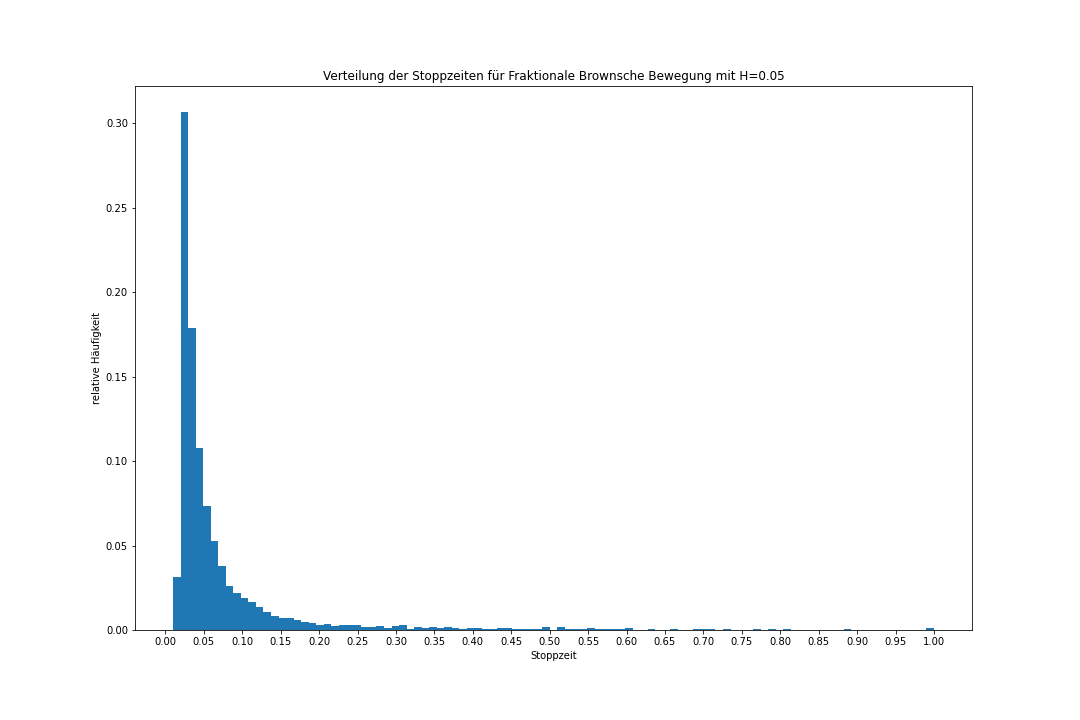
\includegraphics[width=.5\textwidth]{signatur/histogram_0_05.png}}
        \subfigure[Hybridmethode mit $H=0.05$]{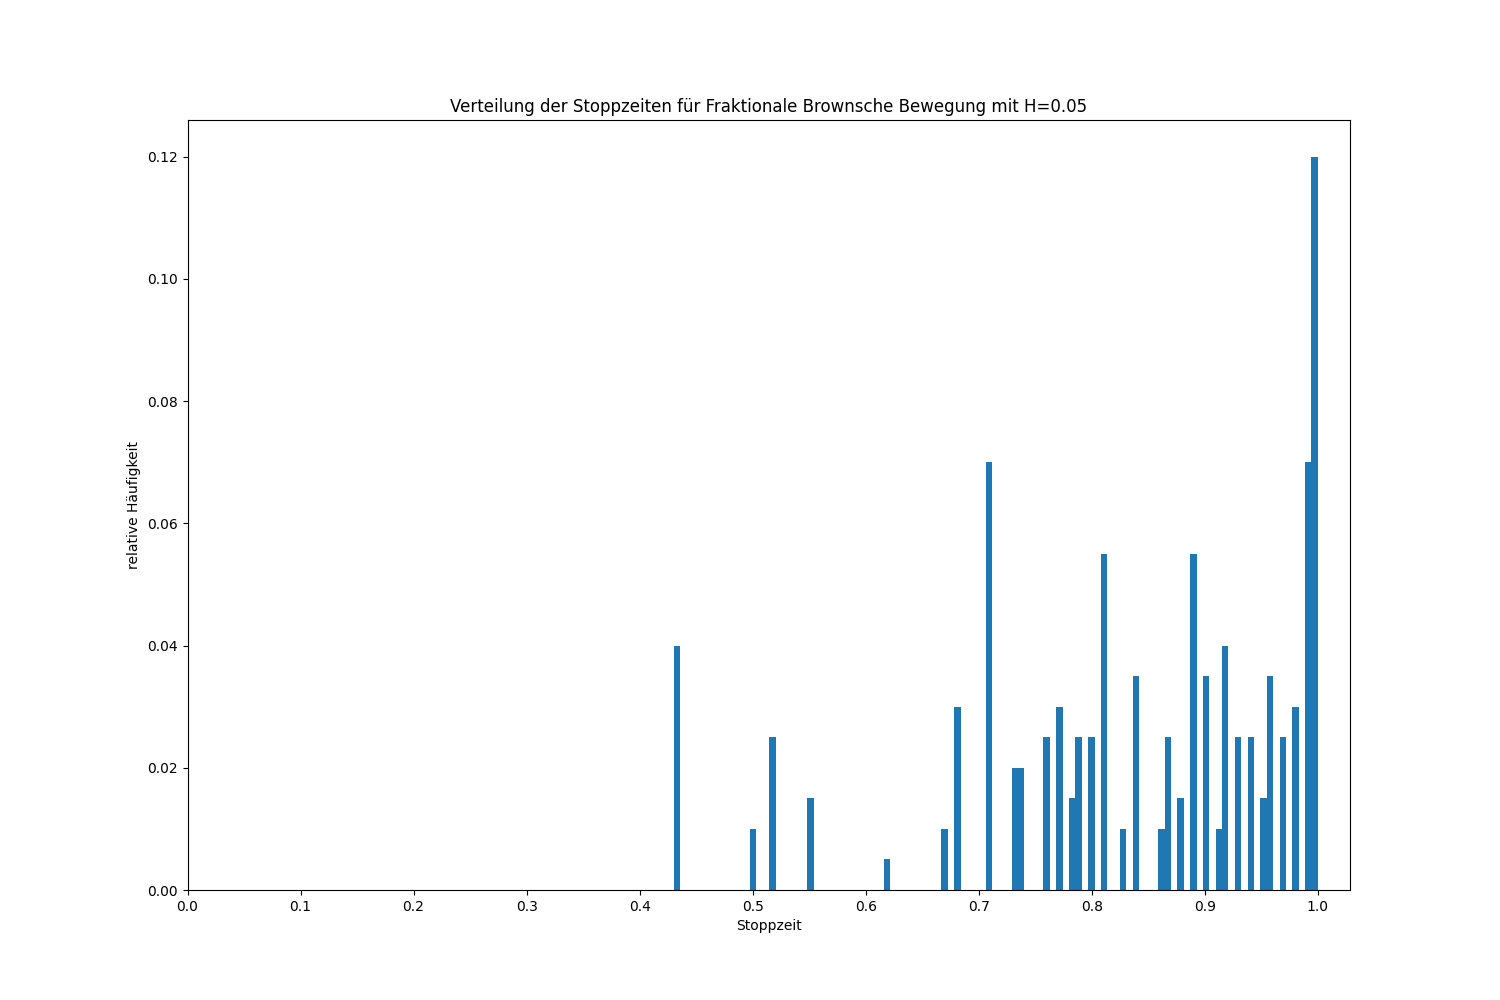
\includegraphics[width=.5\textwidth]{hybrid/histogram_0_05.png}}
        \subfigure[Signaturmethode mit $H=0.1$]{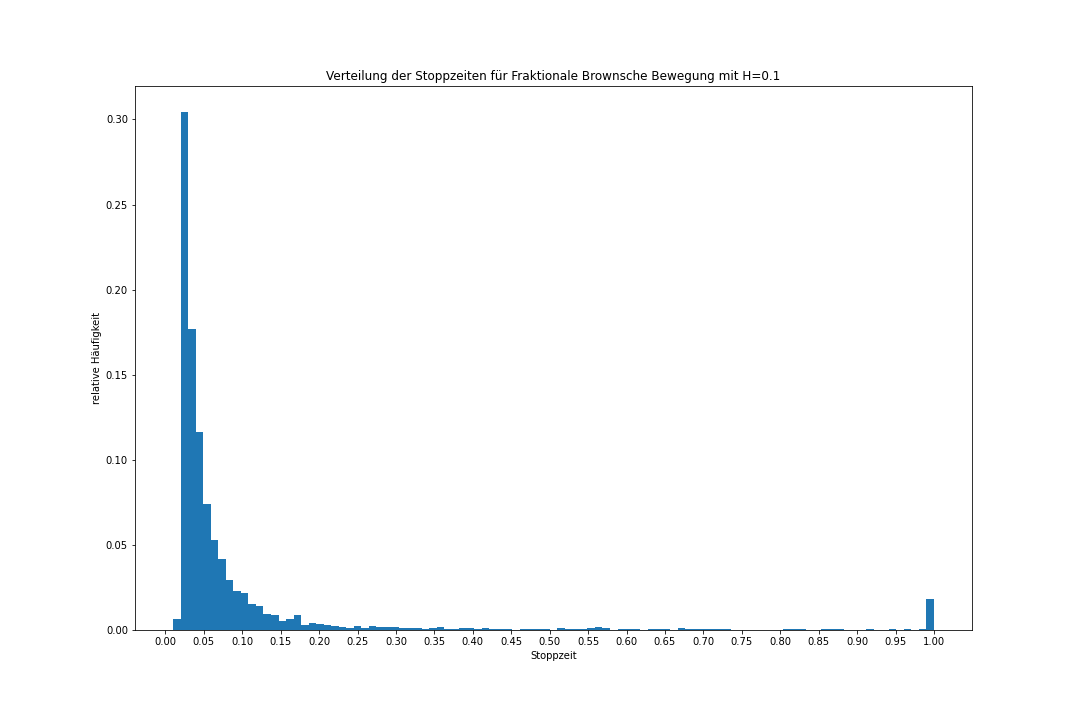
\includegraphics[width=.5\textwidth]{signatur/histogram_0_1.png}}
        \subfigure[Hybridmethode mit $H=0.1$]{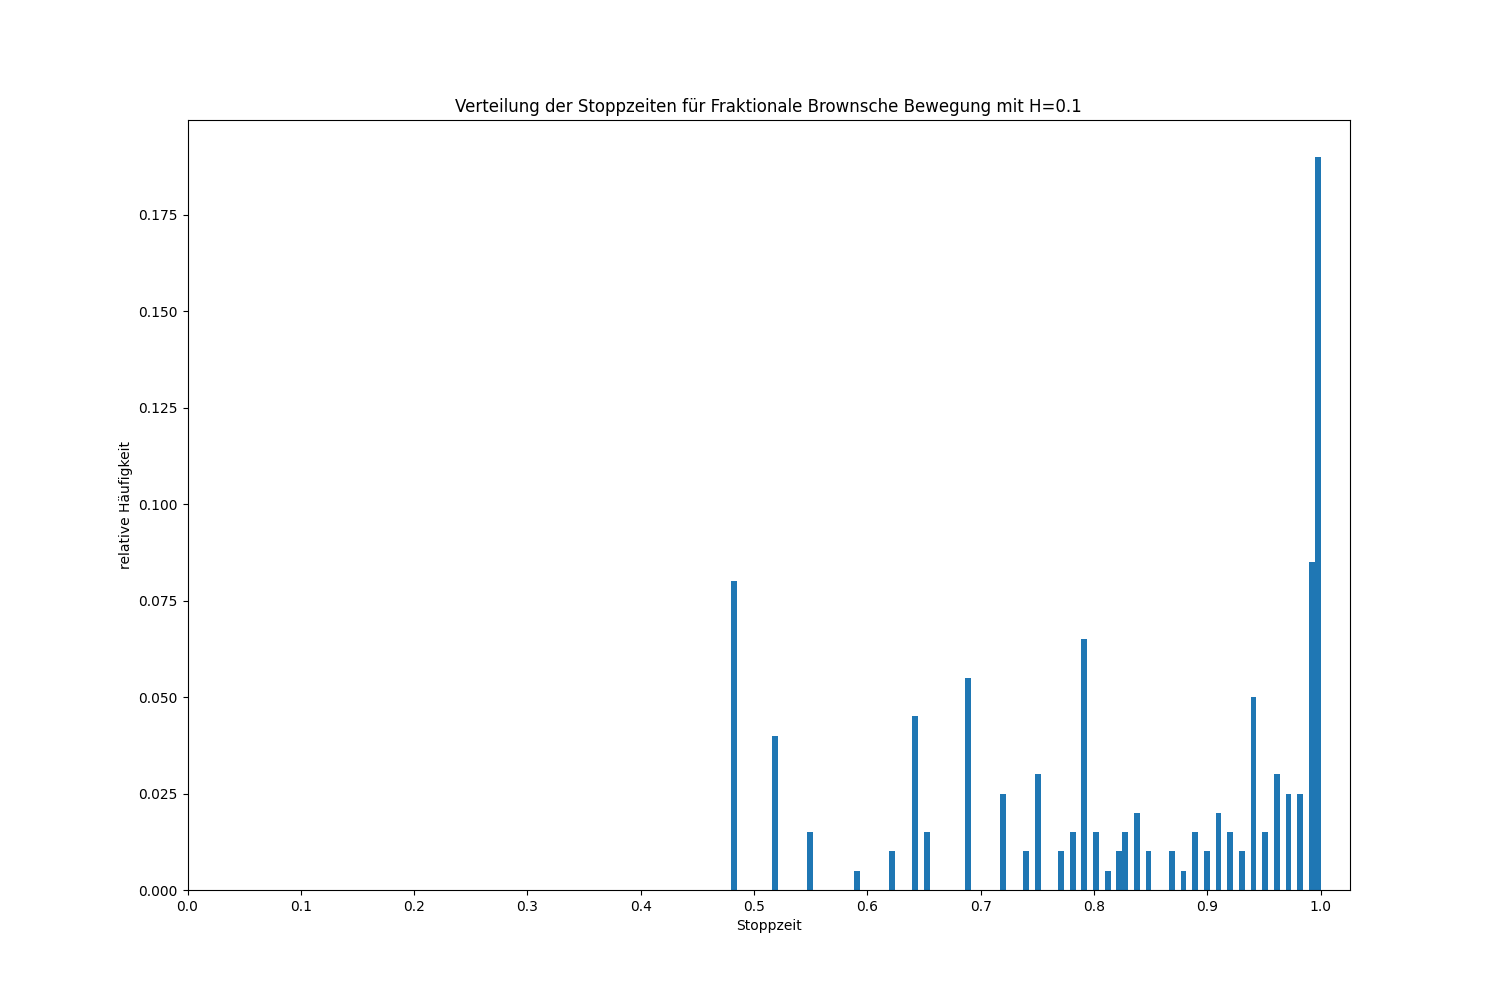
\includegraphics[width=.5\textwidth]{hybrid/histogram_0_1.png}}
        \subfigure[Signaturmethode mit $H=0.15$]{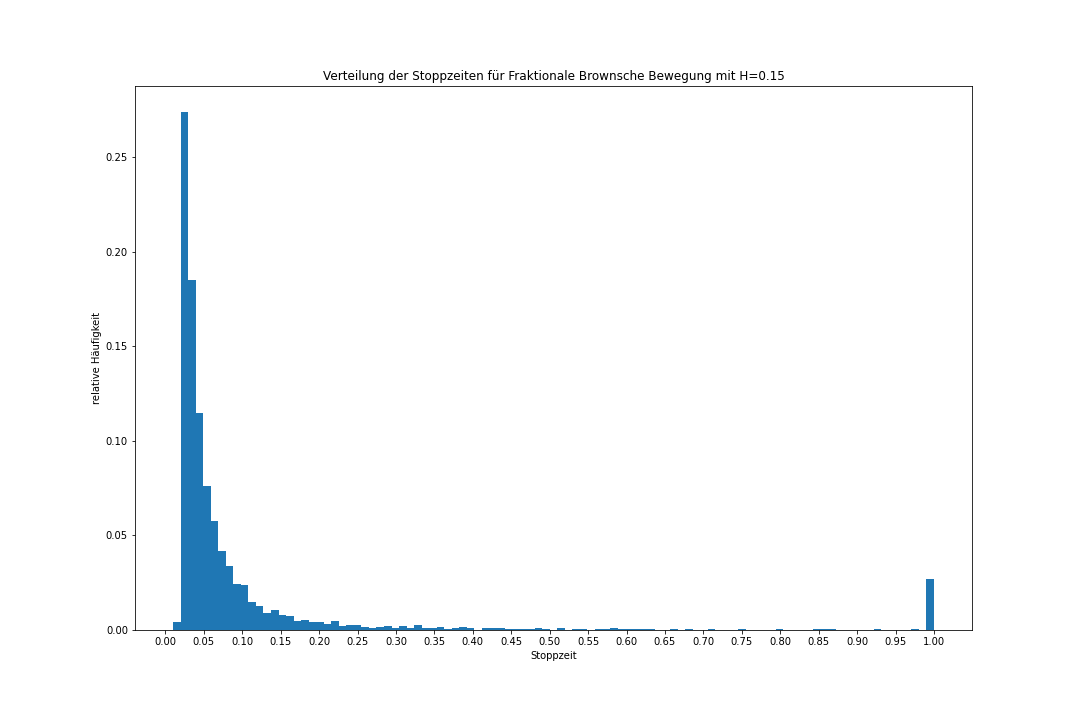
\includegraphics[width=.5\textwidth]{signatur/histogram_0_15.png}}
        \subfigure[Hybridmethode mit $H=0.15$]{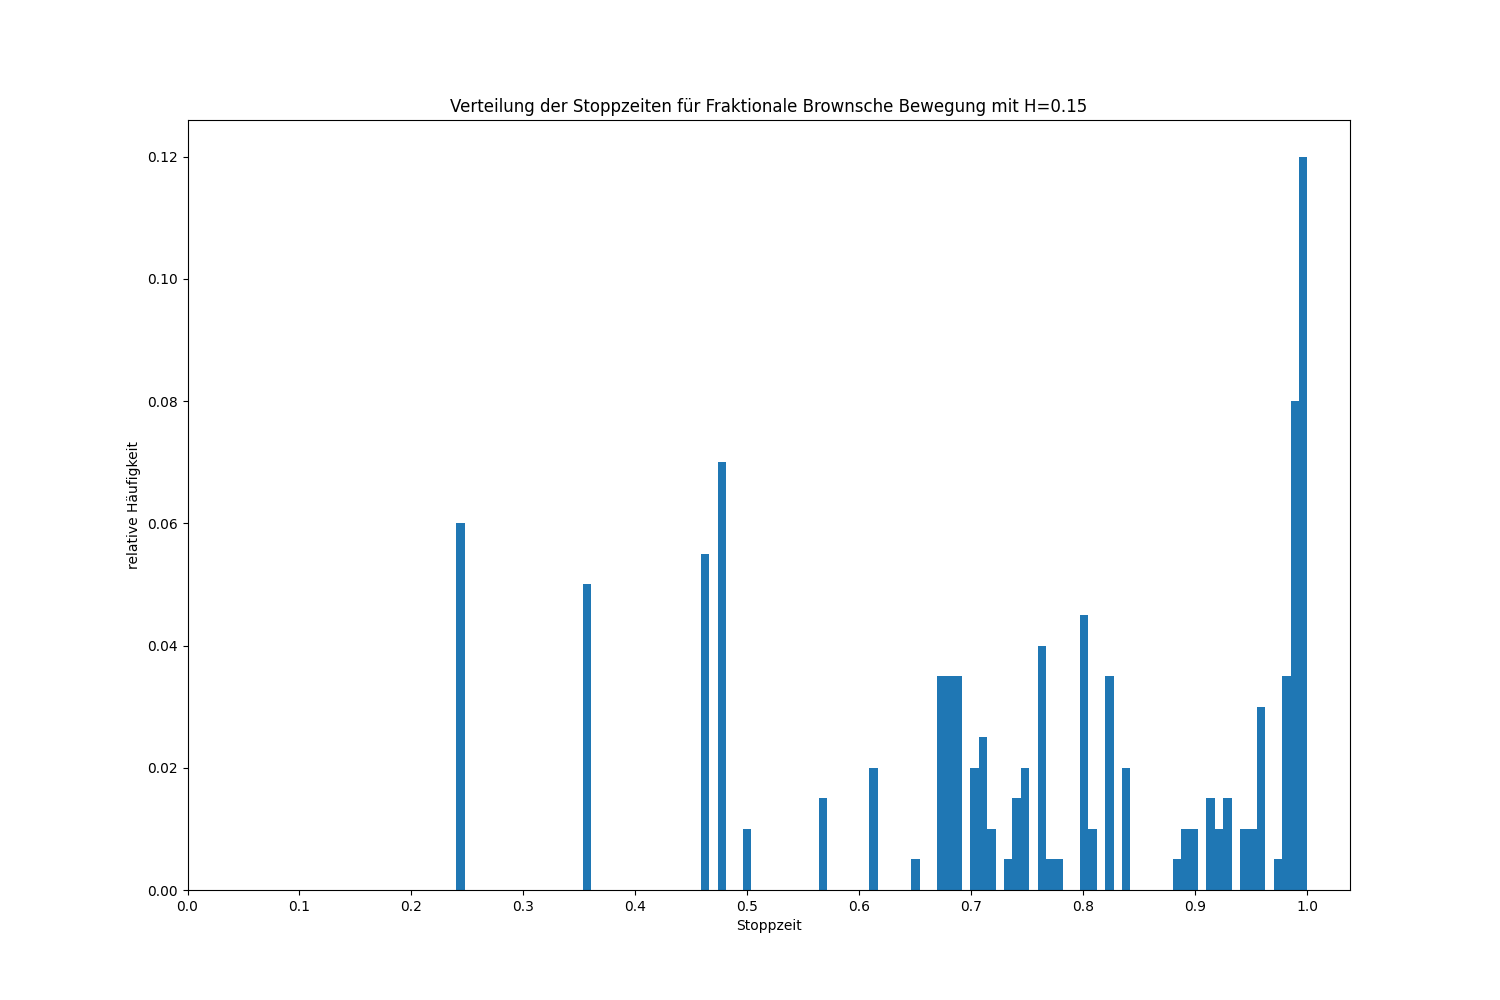
\includegraphics[width=.5\textwidth]{hybrid/histogram_0_15.png}}
        \subfigure[Signaturmethode mit $H=0.2$]{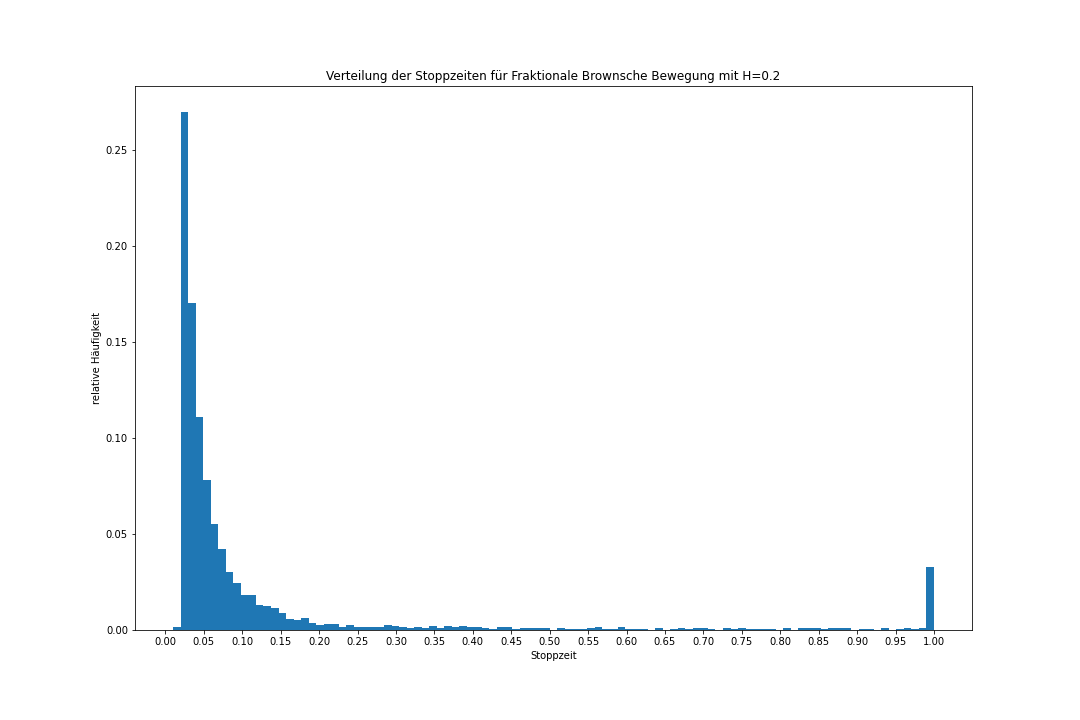
\includegraphics[width=.5\textwidth]{signatur/histogram_0_2.png}}
        \subfigure[Hybridmethode mit $H=0.2$]{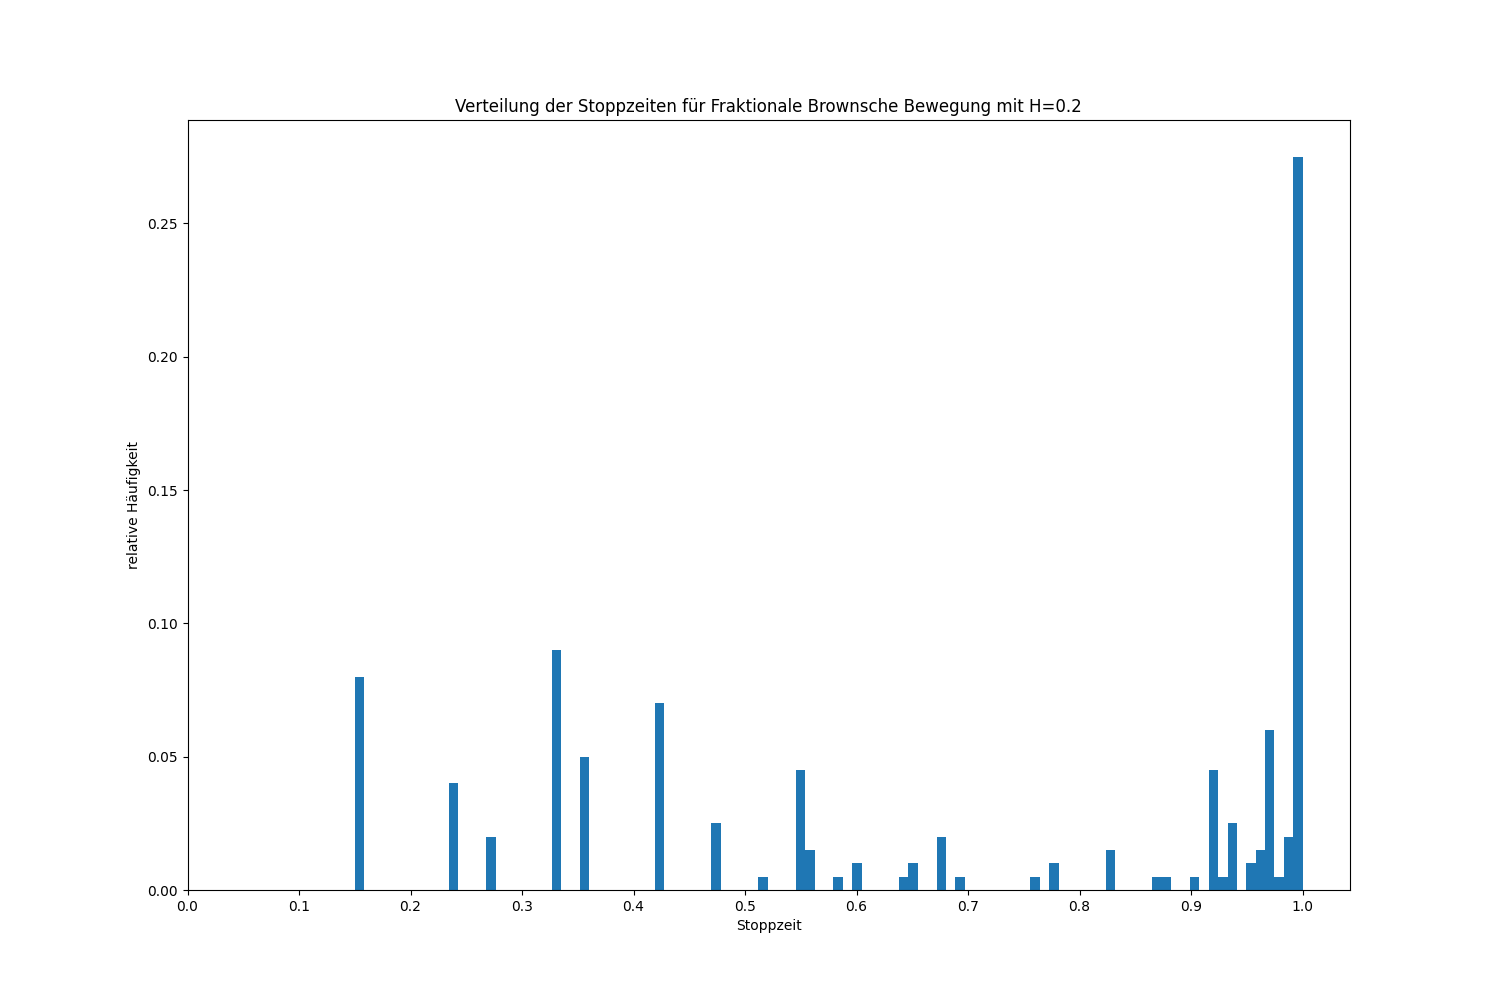
\includegraphics[width=.5\textwidth]{hybrid/histogram_0_2.png}}
      \end{figure}
      \begin{figure}[H]
        \subfigure[Signaturmethode mit $H=0.25$]{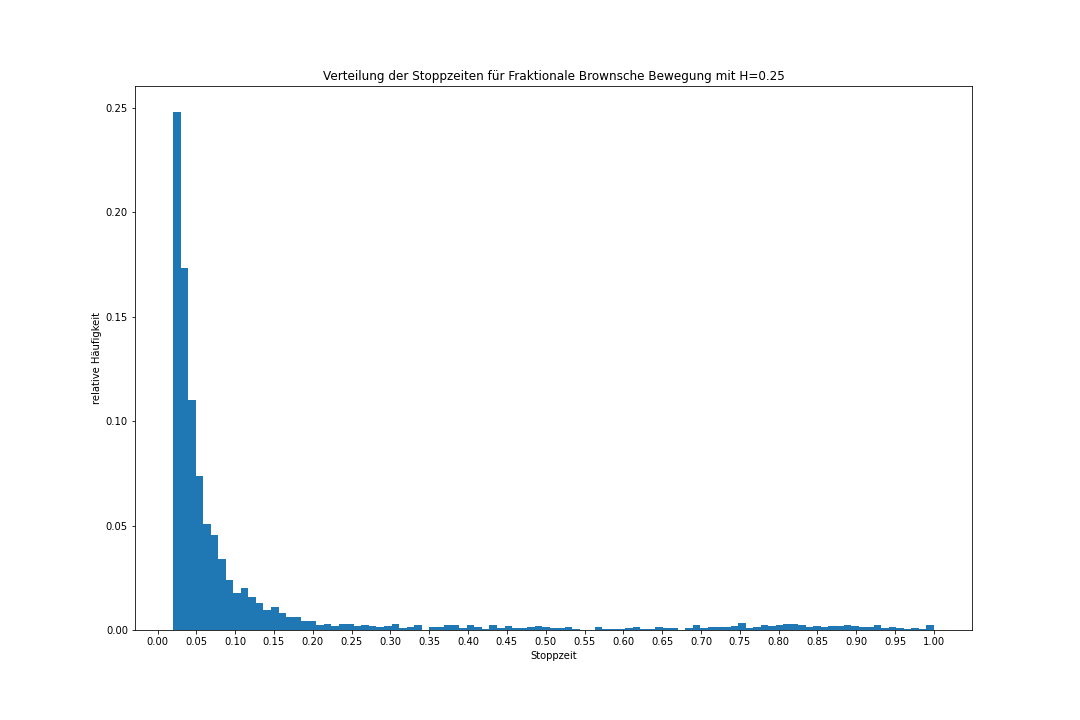
\includegraphics[width=.5\textwidth]{signatur/histogram_0_25.png}}
        \subfigure[Hybridmethode mit $H=0.25$]{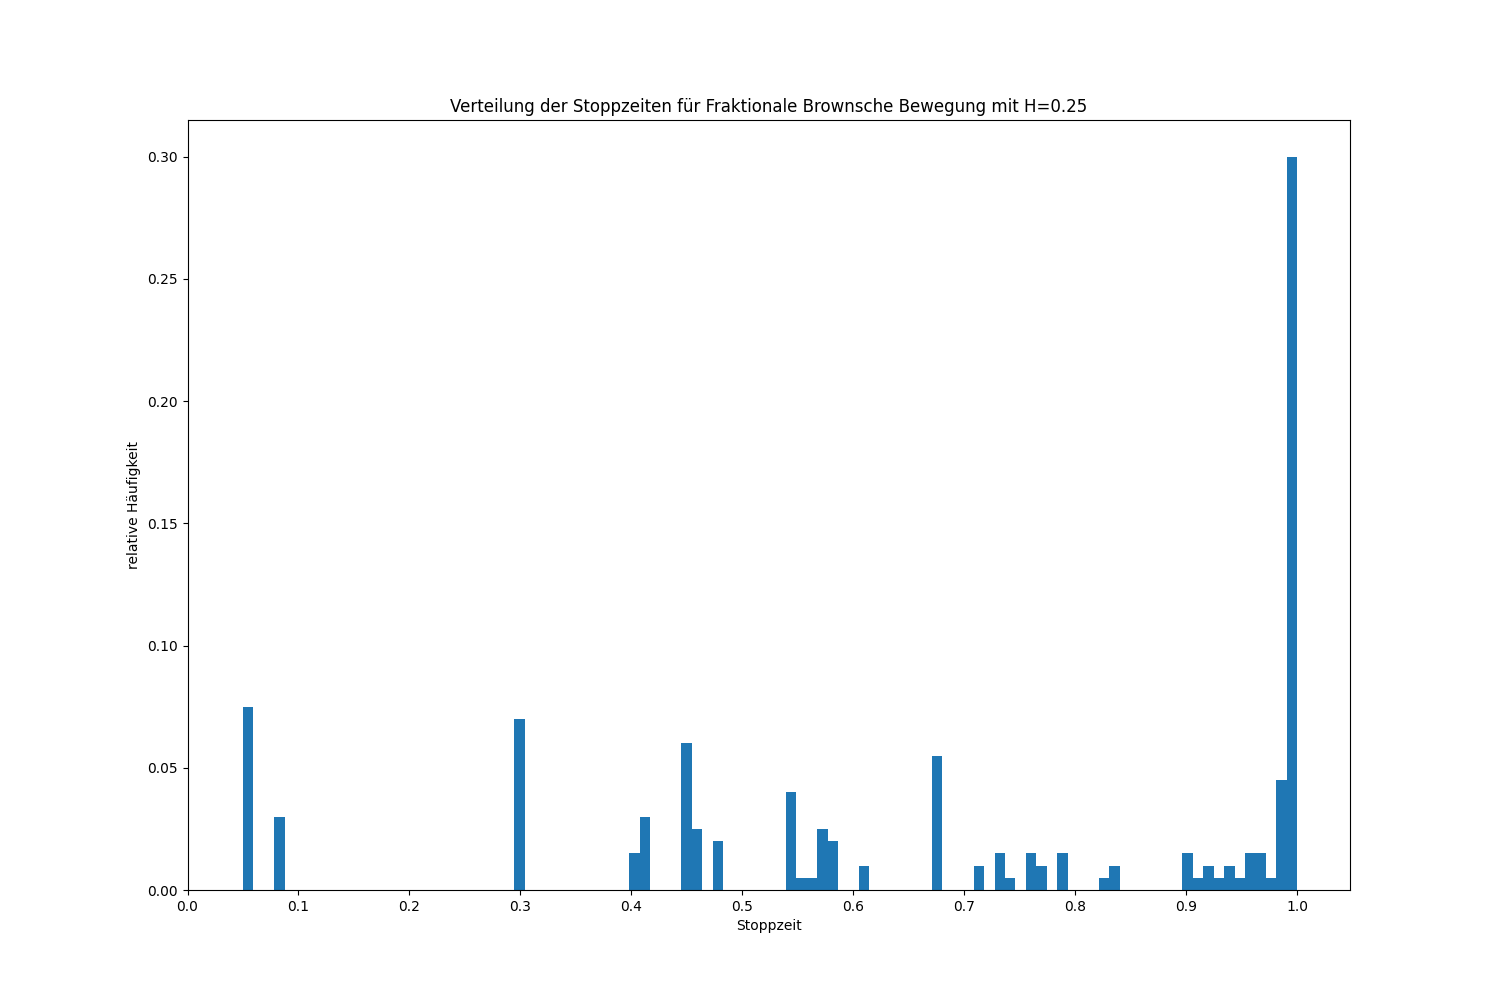
\includegraphics[width=.5\textwidth]{hybrid/histogram_0_25.png}}
        \subfigure[Signaturmethode mit $H=0.3$]{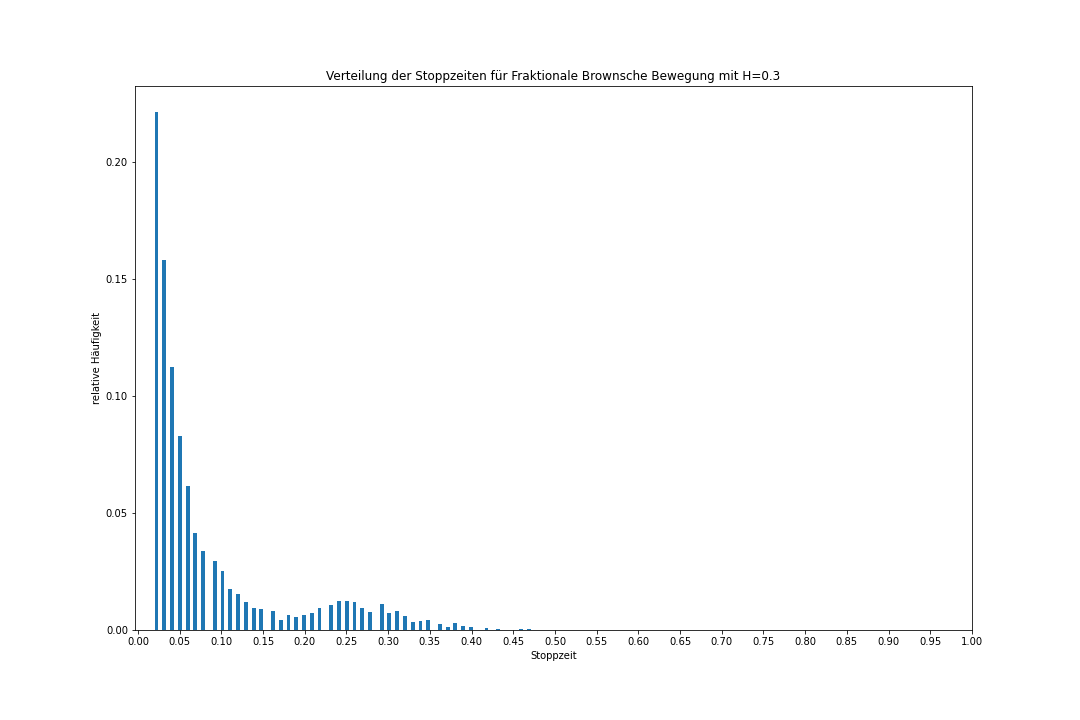
\includegraphics[width=.5\textwidth]{signatur/histogram_0_3.png}}
        \subfigure[Hybridmethode mit $H=0.3$]{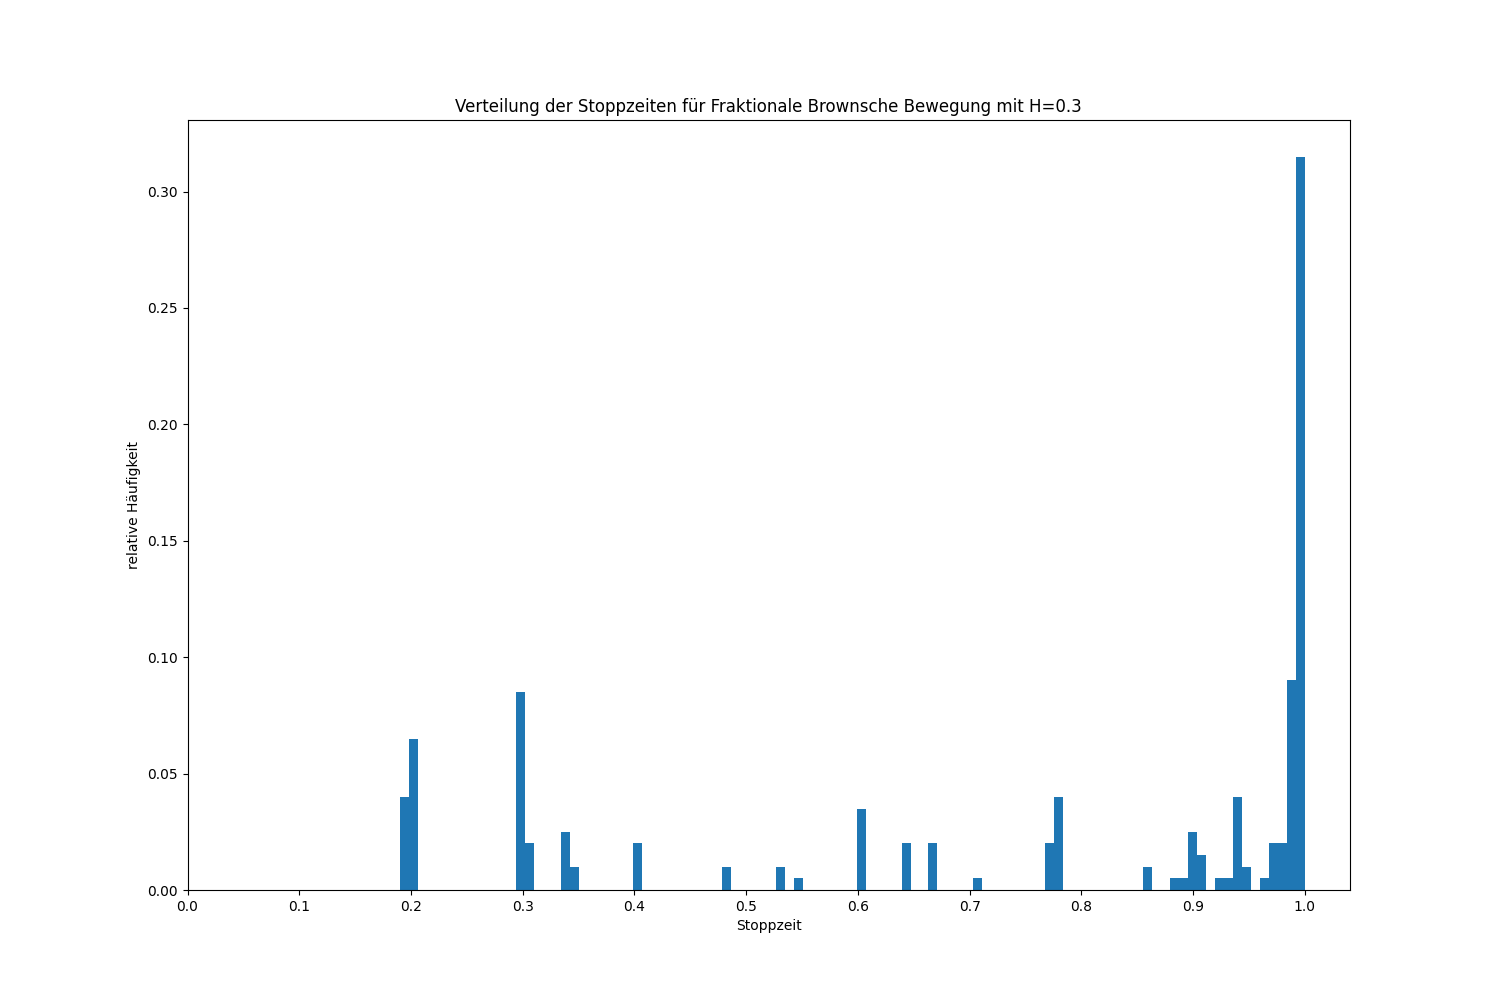
\includegraphics[width=.5\textwidth]{hybrid/histogram_0_3.png}}
        \subfigure[Signaturmethode mit $H=0.35$]{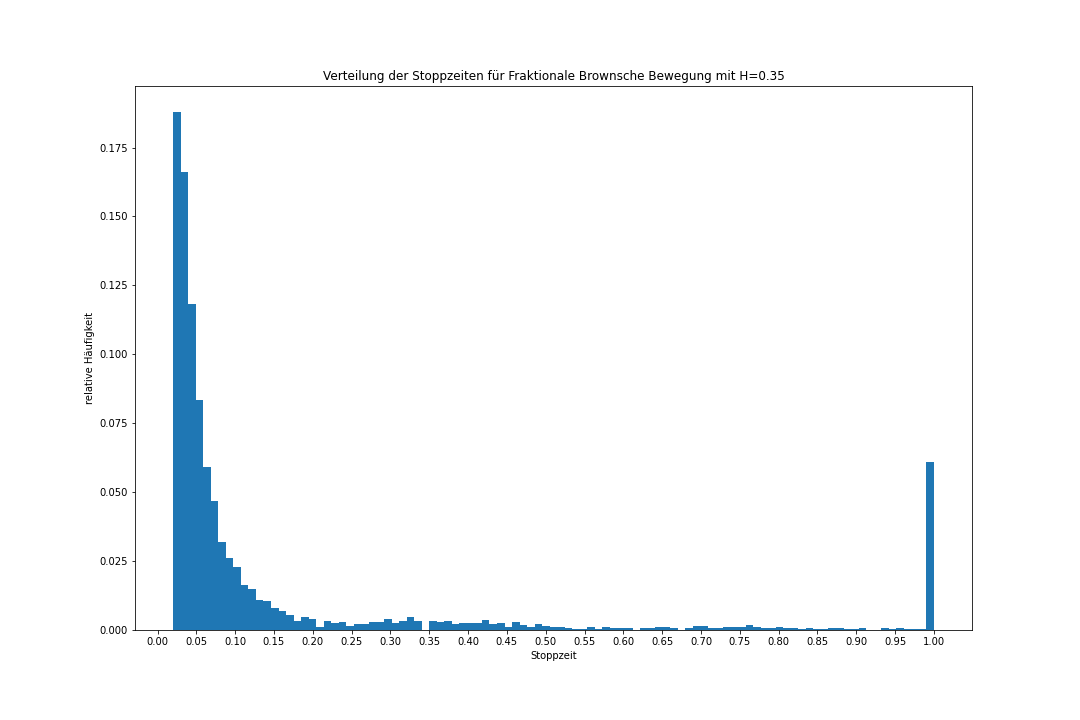
\includegraphics[width=.5\textwidth]{signatur/histogram_0_35.png}}
        \subfigure[Hybridmethode mit $H=0.35$]{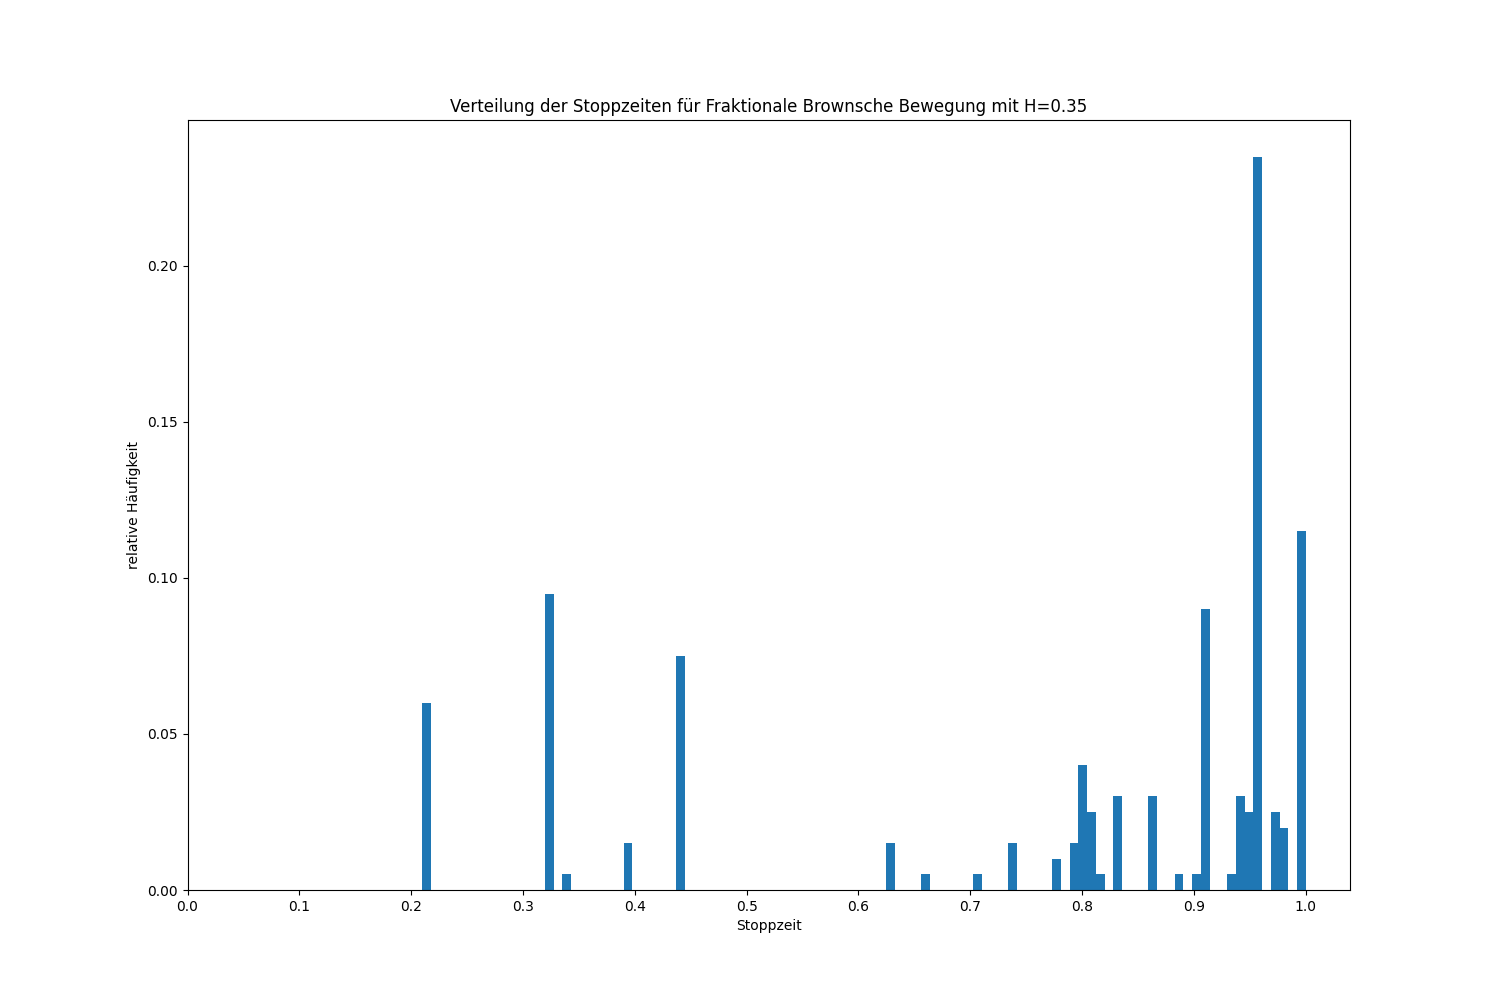
\includegraphics[width=.5\textwidth]{hybrid/histogram_0_35.png}}
        \subfigure[Signaturmethode mit $H=0.4$]{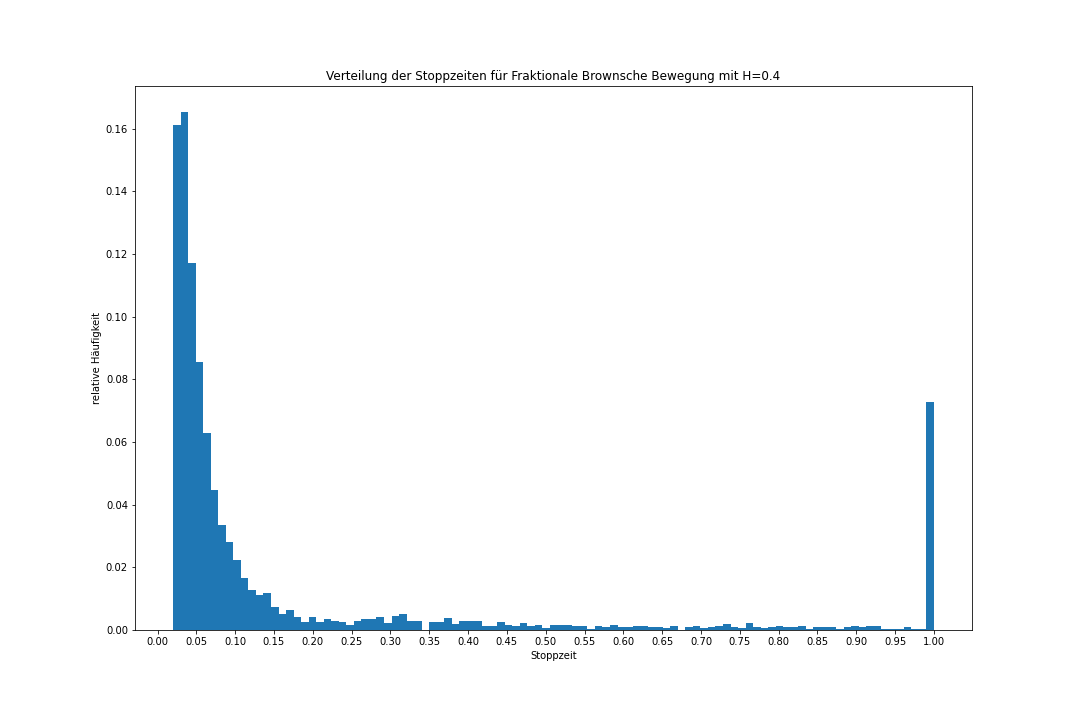
\includegraphics[width=.5\textwidth]{signatur/histogram_0_4.png}}
        \subfigure[Hybridmethode mit $H=0.4$]{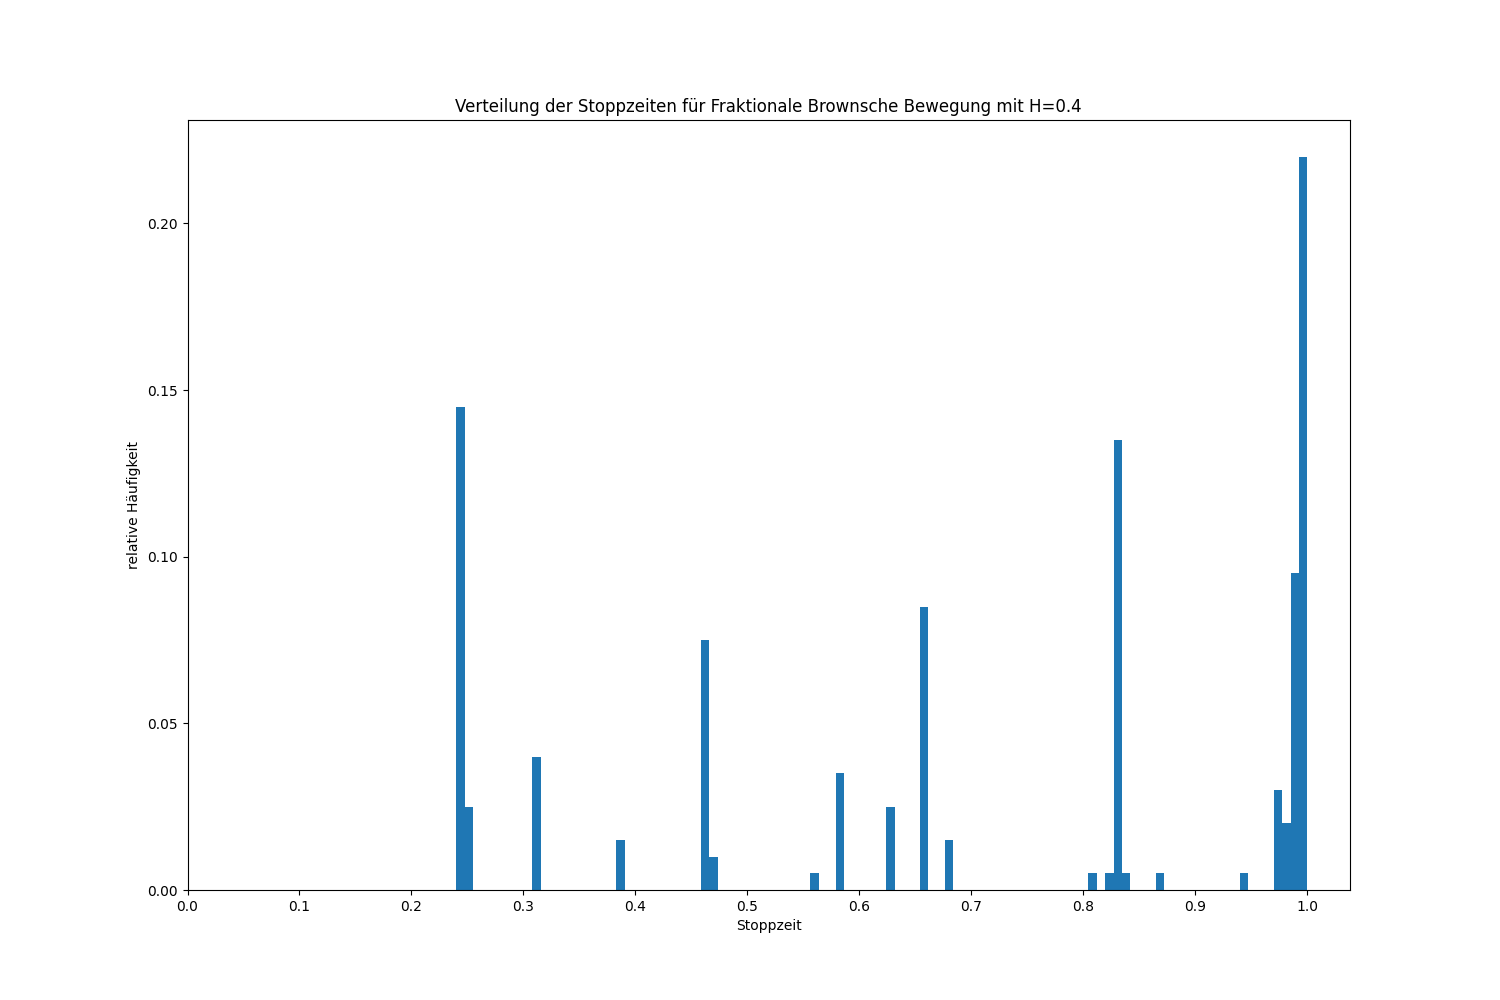
\includegraphics[width=.5\textwidth]{hybrid/histogram_0_4.png}}
      \end{figure}
      \begin{figure}[H]
        \subfigure[Signaturmethode mit $H=0.45$]{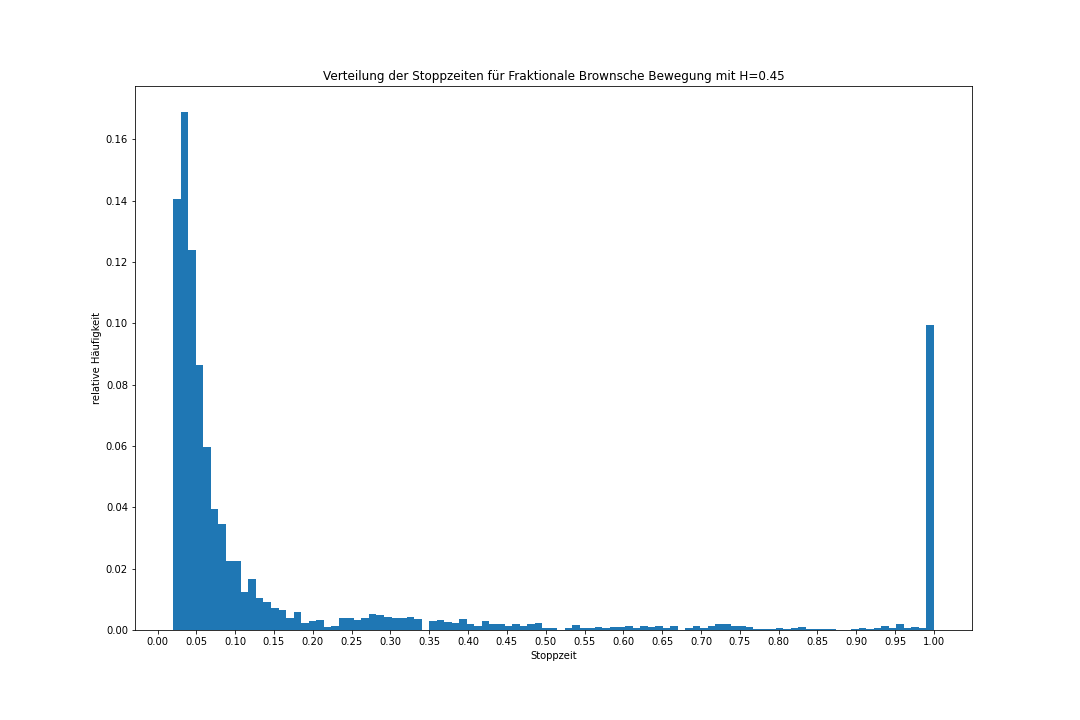
\includegraphics[width=.5\textwidth]{signatur/histogram_0_45.png}}
        \subfigure[Hybridmethode mit $H=0.45$]{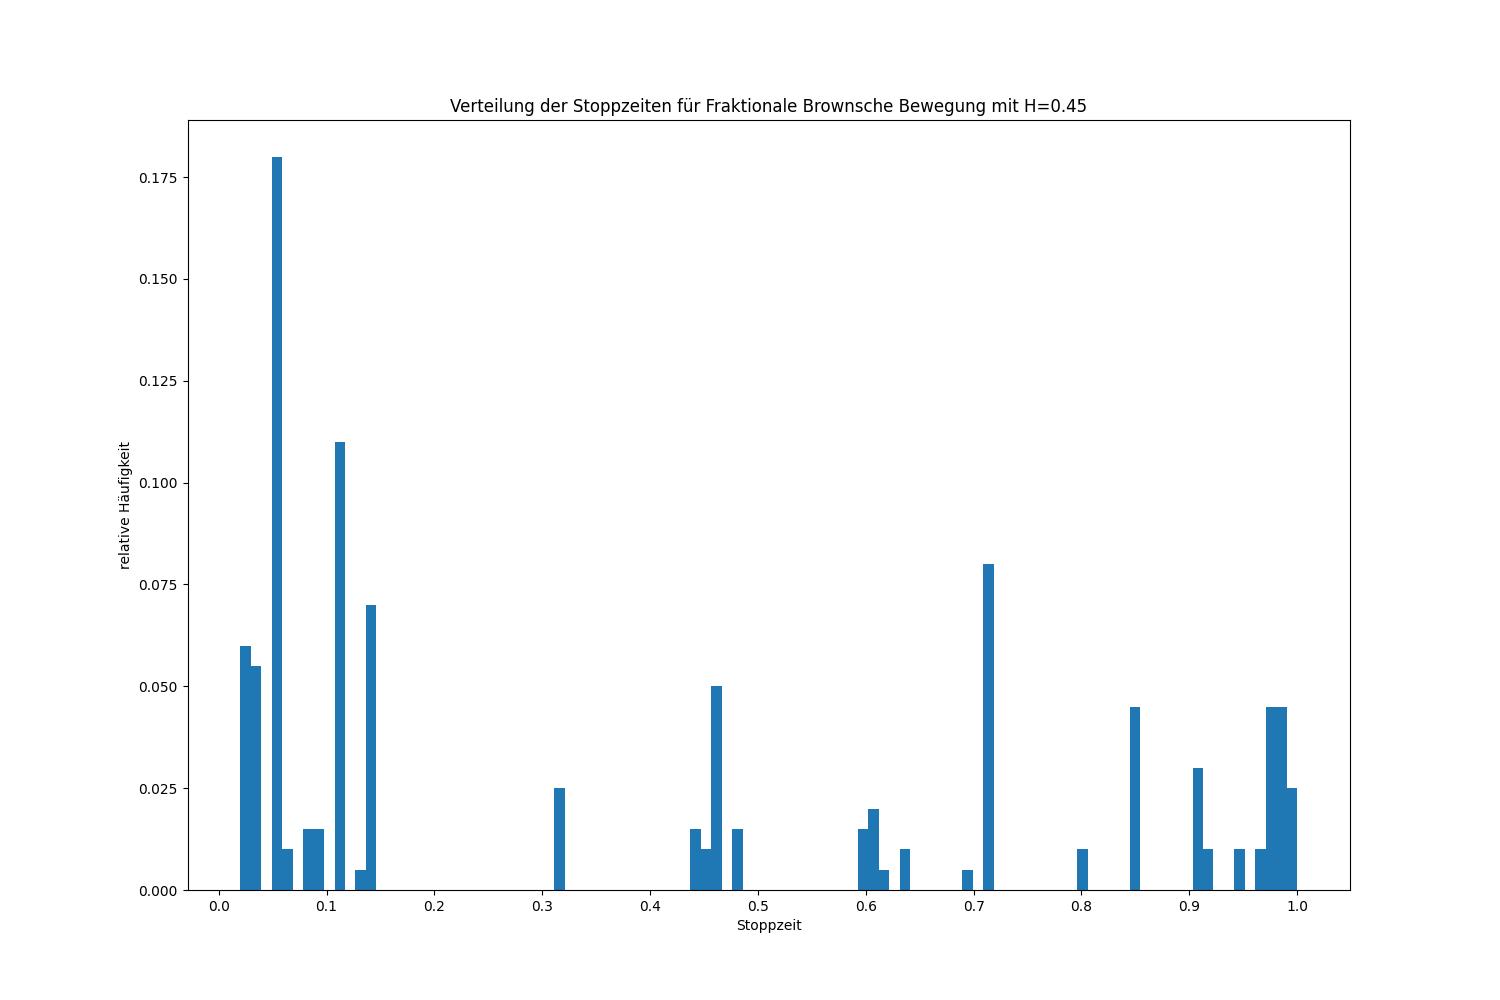
\includegraphics[width=.5\textwidth]{hybrid/histogram_0_45.png}}
        \subfigure[Signaturmethode mit $H=0.5$]{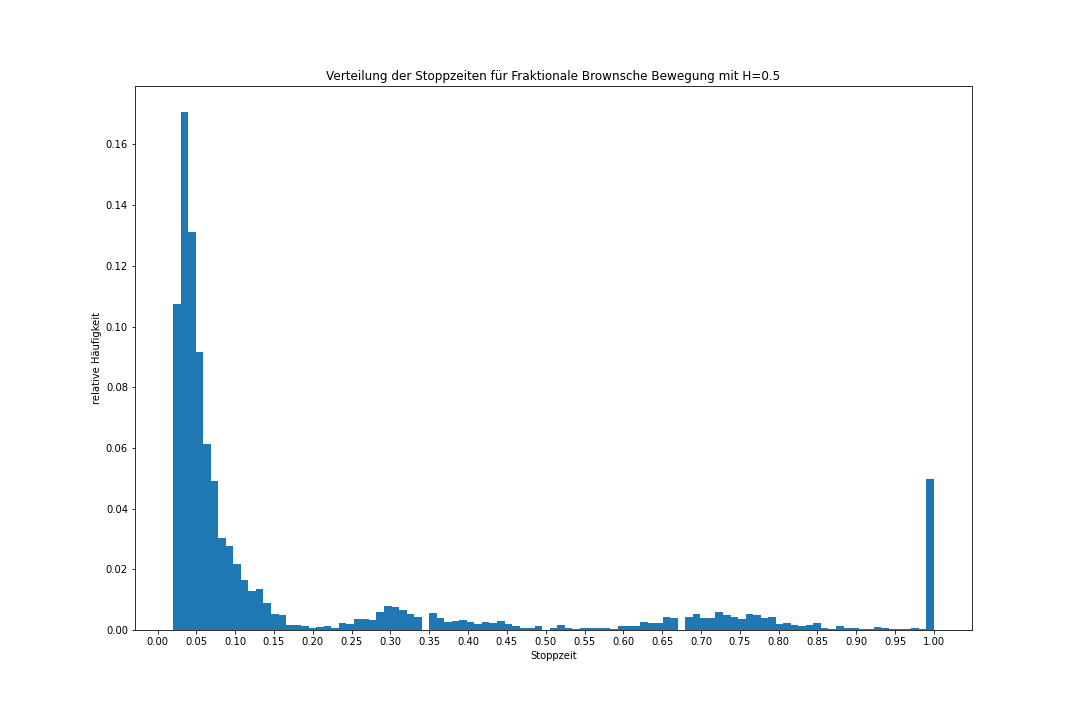
\includegraphics[width=.5\textwidth]{signatur/histogram_0_5.png}}
        \subfigure[Hybridmethode mit $H=0.5$]{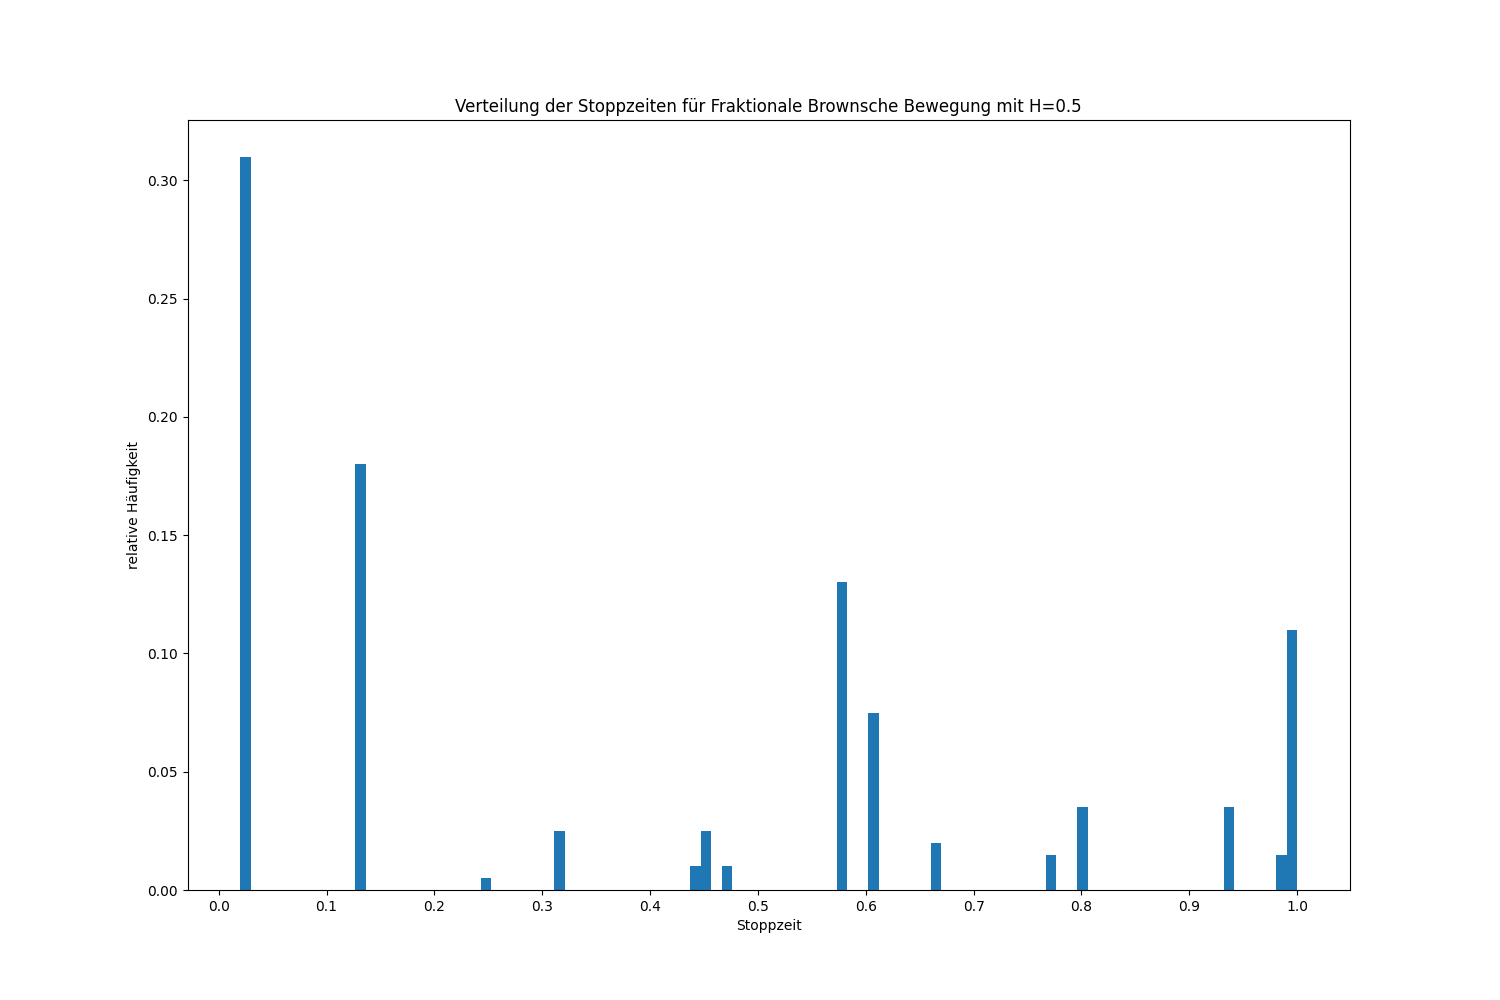
\includegraphics[width=.5\textwidth]{hybrid/histogram_0_5.png}}
        \subfigure[Signaturmethode mit $H=0.55$]{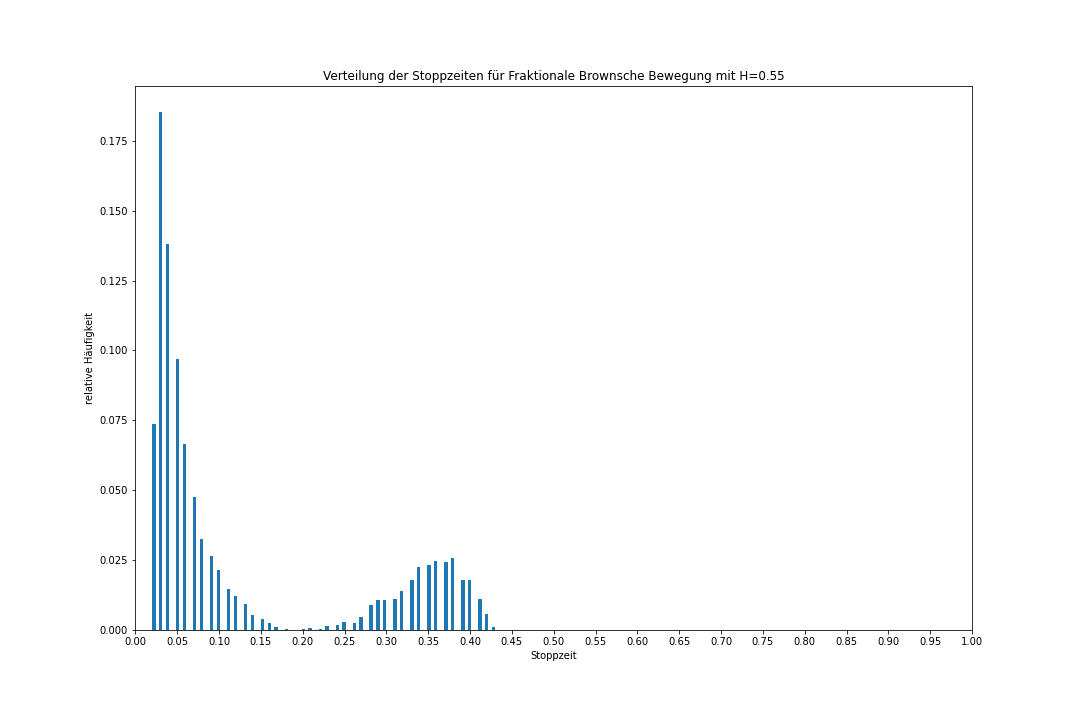
\includegraphics[width=.5\textwidth]{signatur/histogram_0_55.png}}
        \subfigure[Hybridmethode mit $H=0.55$]{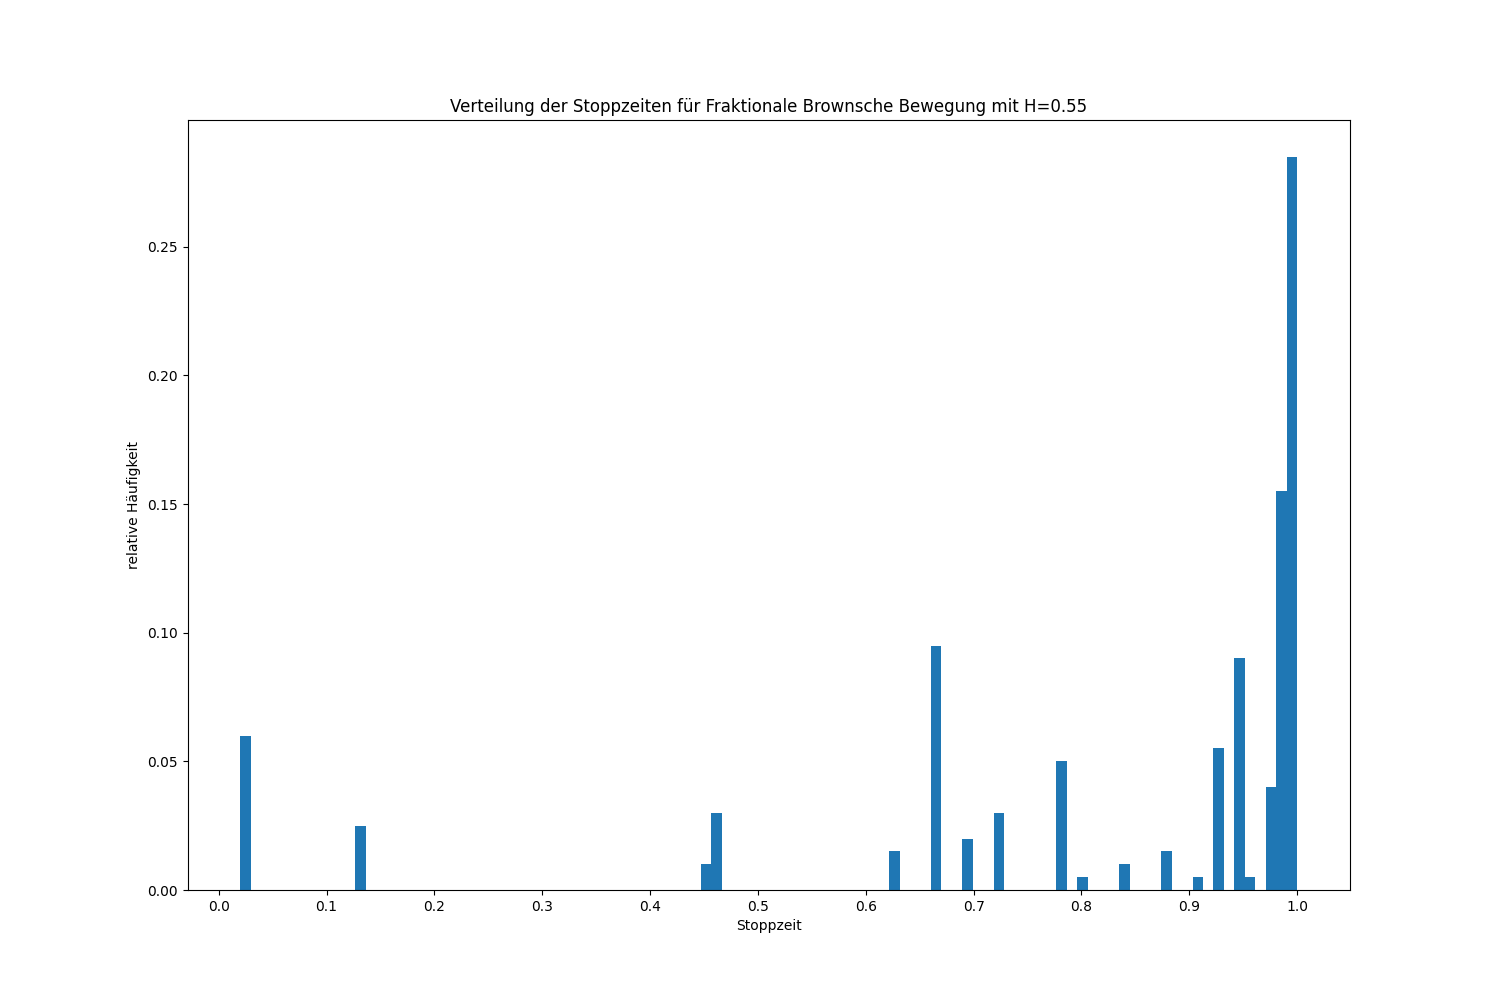
\includegraphics[width=.5\textwidth]{hybrid/histogram_0_55.png}}
        \subfigure[Signaturmethode mit $H=0.6$]{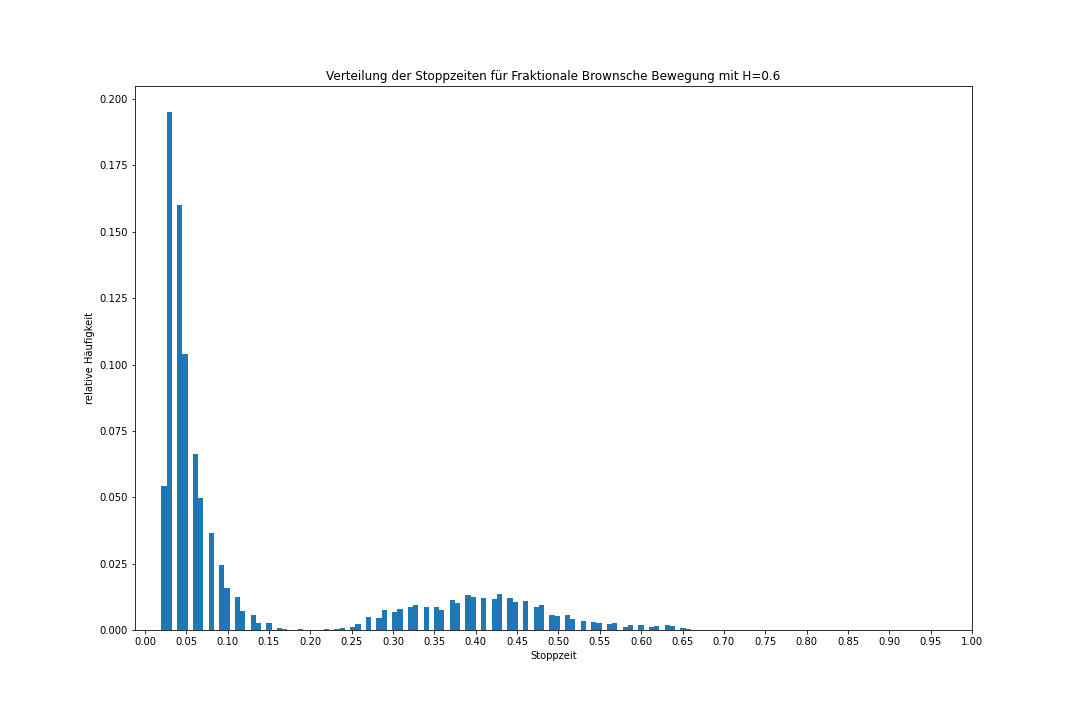
\includegraphics[width=.5\textwidth]{signatur/histogram_0_6.png}}
        \subfigure[Hybridmethode mit $H=0.6$]{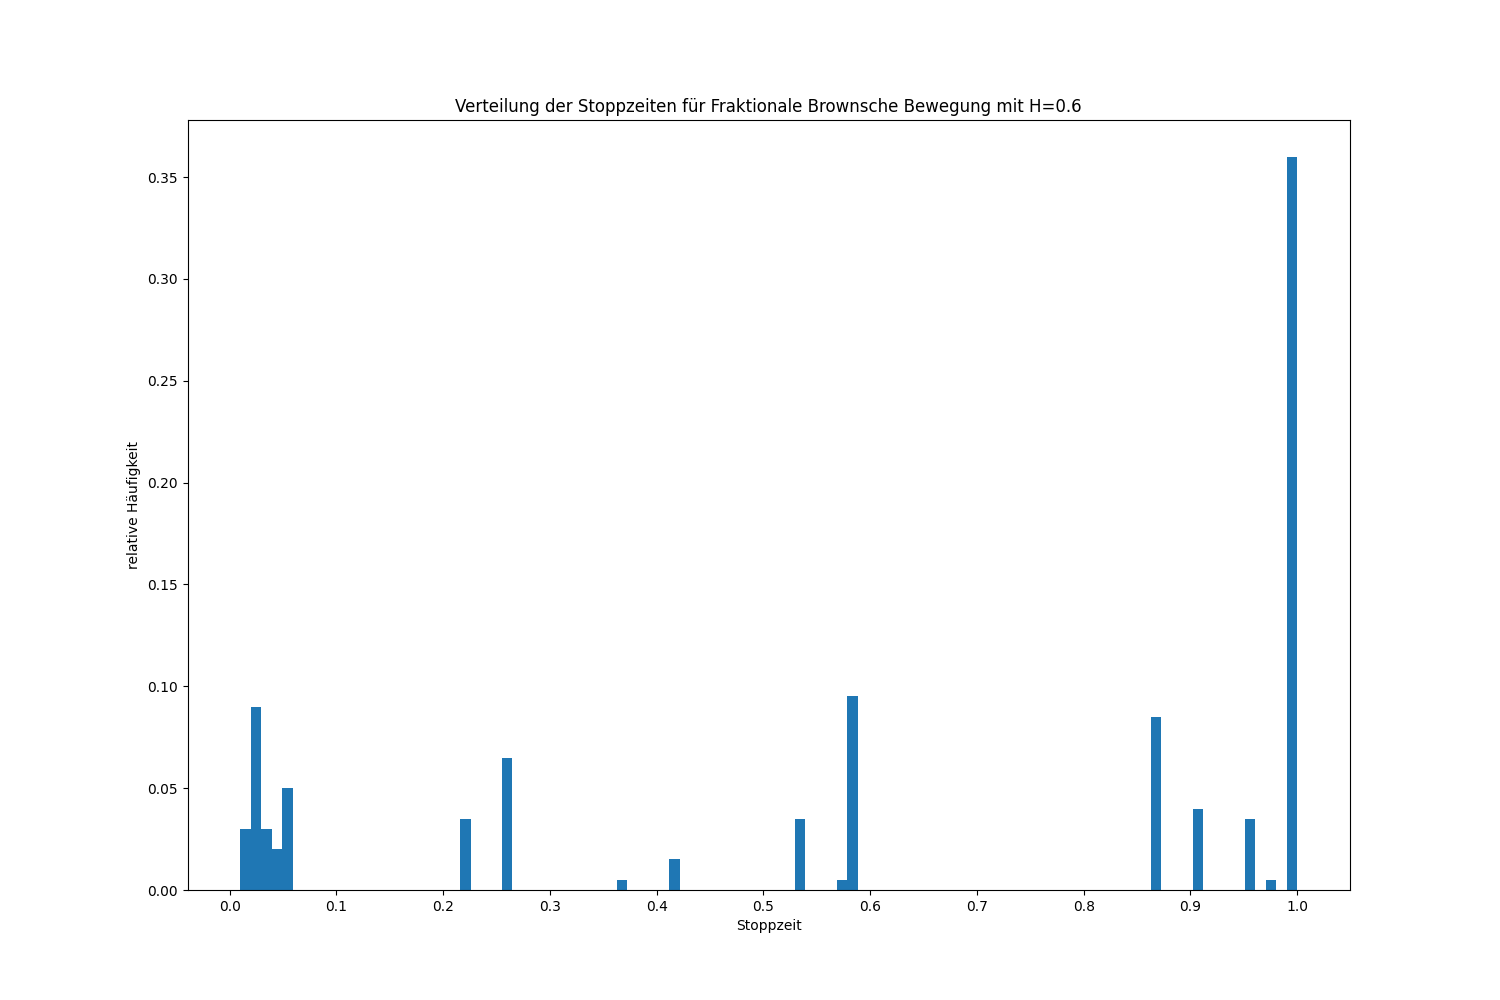
\includegraphics[width=.5\textwidth]{hybrid/histogram_0_6.png}}
      \end{figure}
      \begin{figure}[H]
        \subfigure[Signaturmethode mit $H=0.65$]{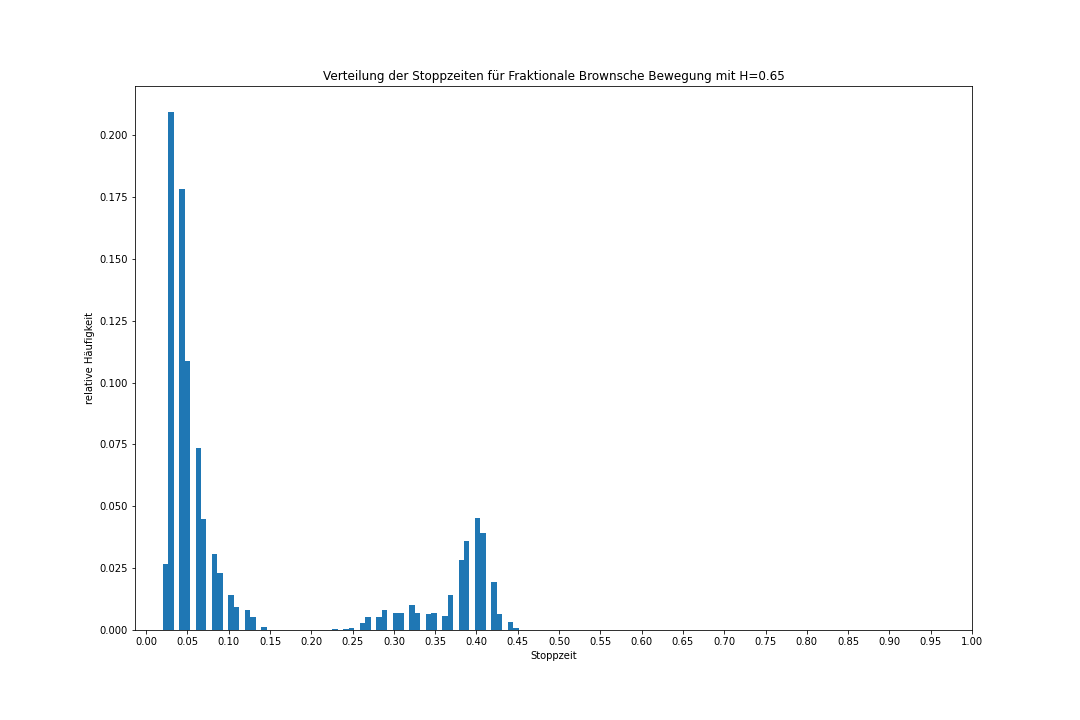
\includegraphics[width=.5\textwidth]{signatur/histogram_0_65.png}}
        \subfigure[Hybridmethode mit $H=0.65$]{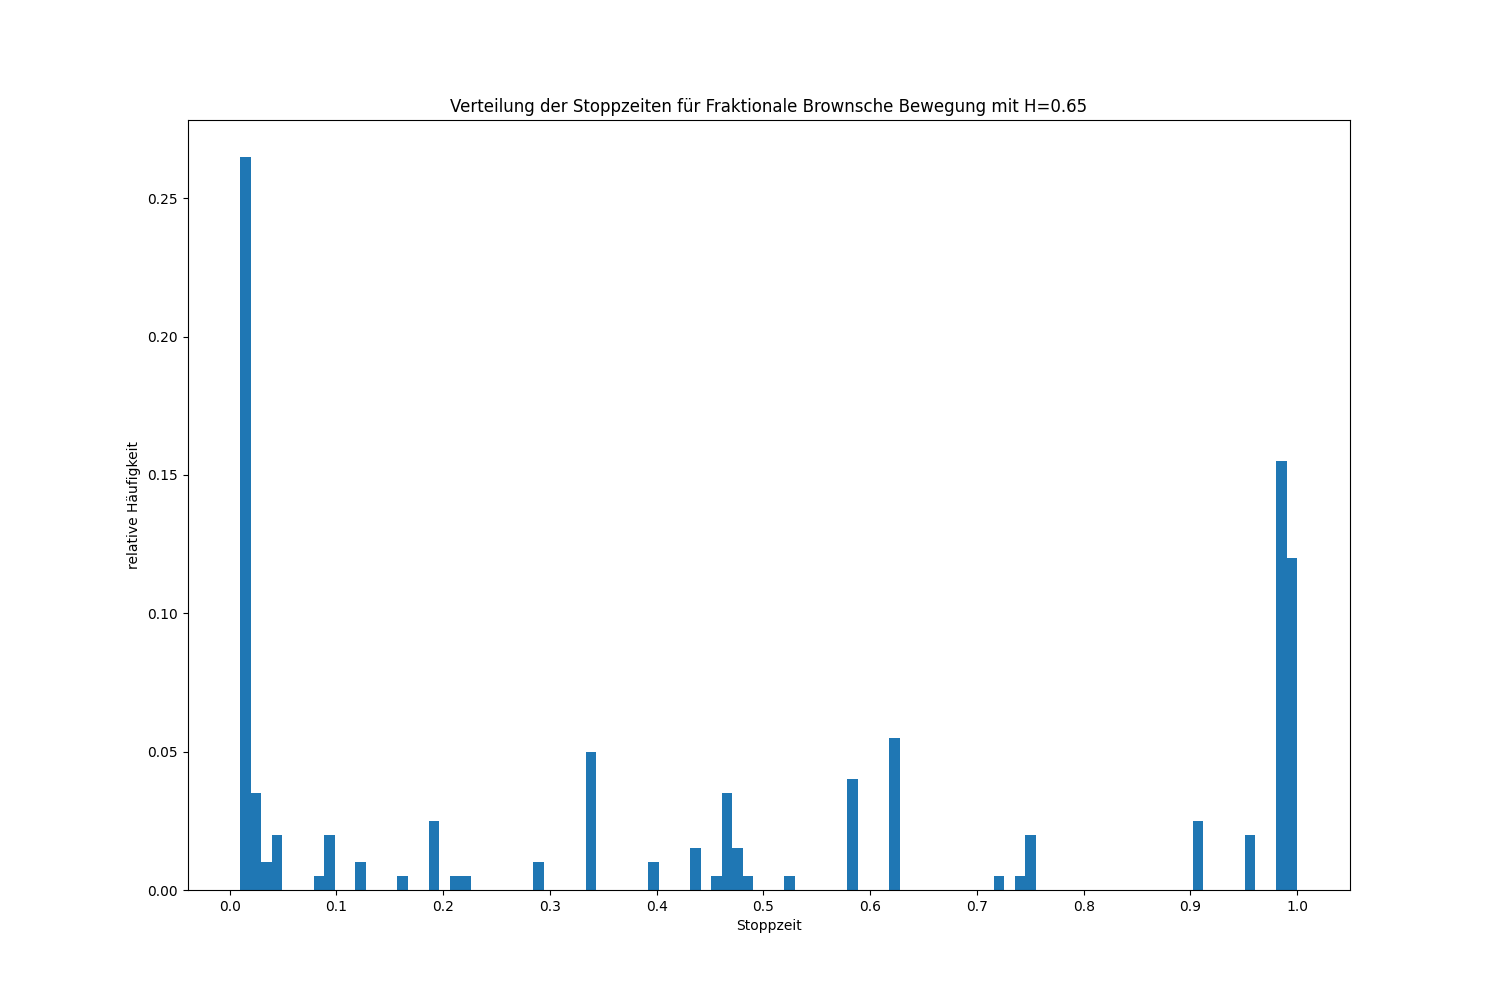
\includegraphics[width=.5\textwidth]{hybrid/histogram_0_65.png}}
        \subfigure[Signaturmethode mit $H=0.7$]{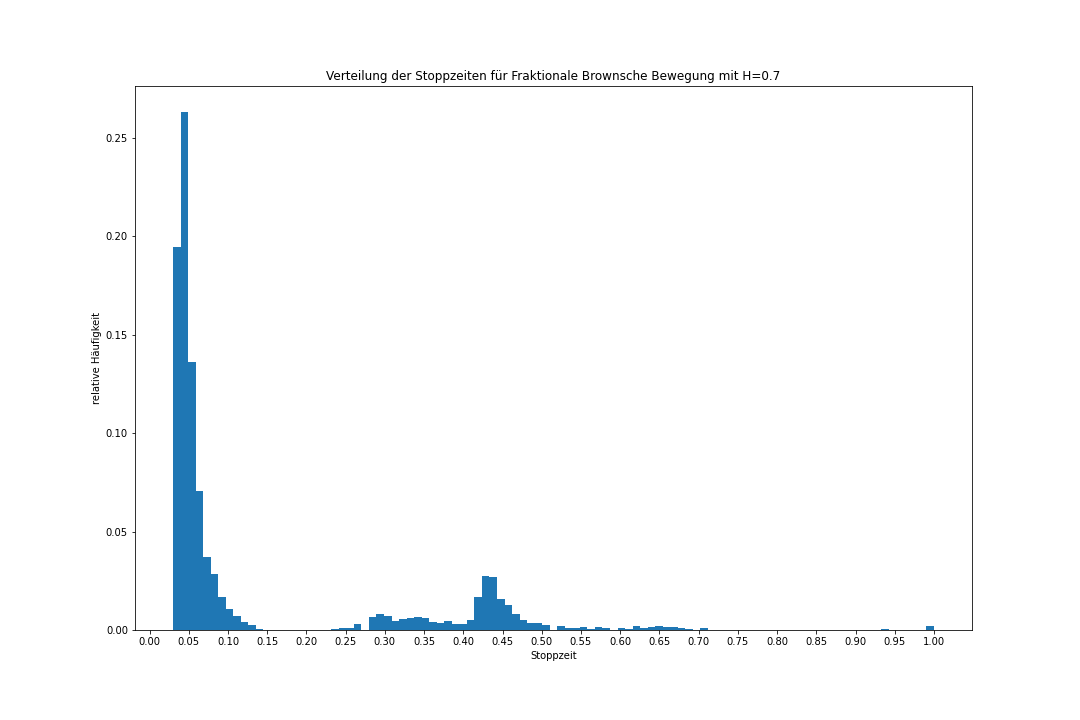
\includegraphics[width=.5\textwidth]{signatur/histogram_0_7.png}}
        \subfigure[Hybridmethode mit $H=0.7$]{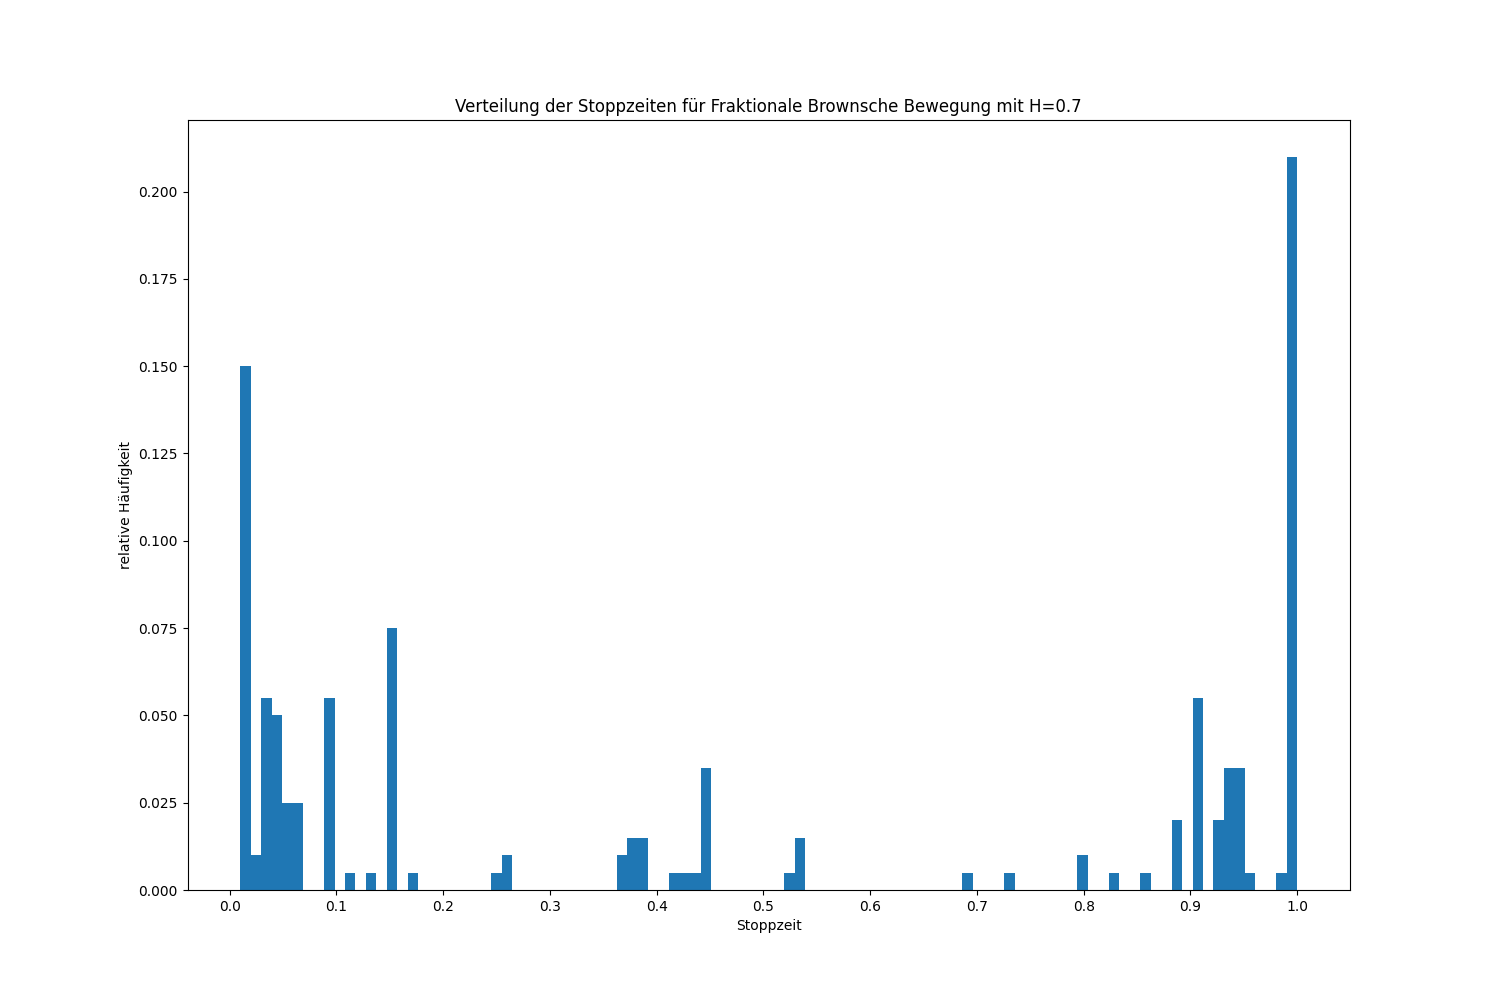
\includegraphics[width=.5\textwidth]{hybrid/histogram_0_7.png}}
        \subfigure[Signaturmethode mit $H=0.75$]{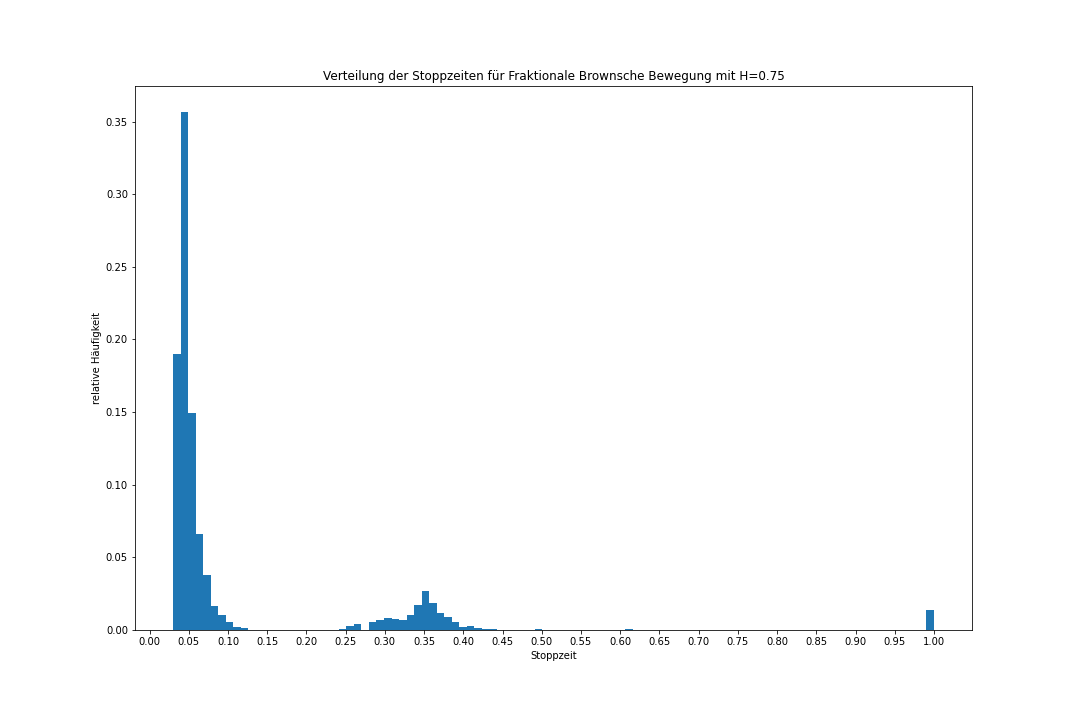
\includegraphics[width=.5\textwidth]{signatur/histogram_0_75.png}}
        \subfigure[Hybridmethode mit $H=0.75$]{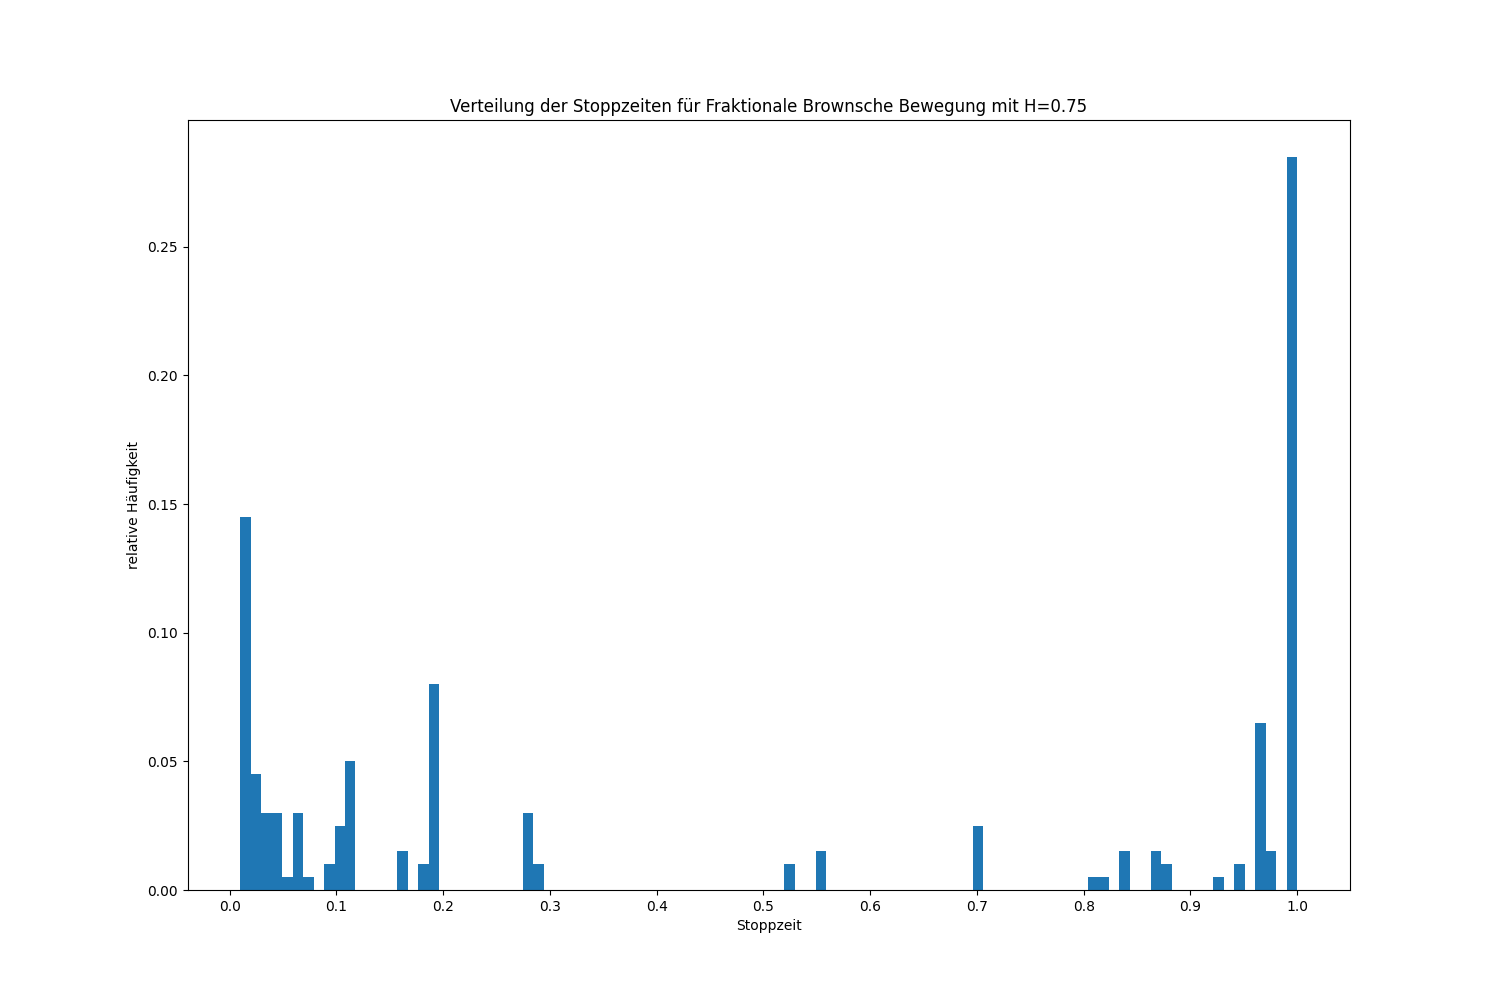
\includegraphics[width=.5\textwidth]{hybrid/histogram_0_75.png}}
        \subfigure[Signaturmethode mit $H=0.8$]{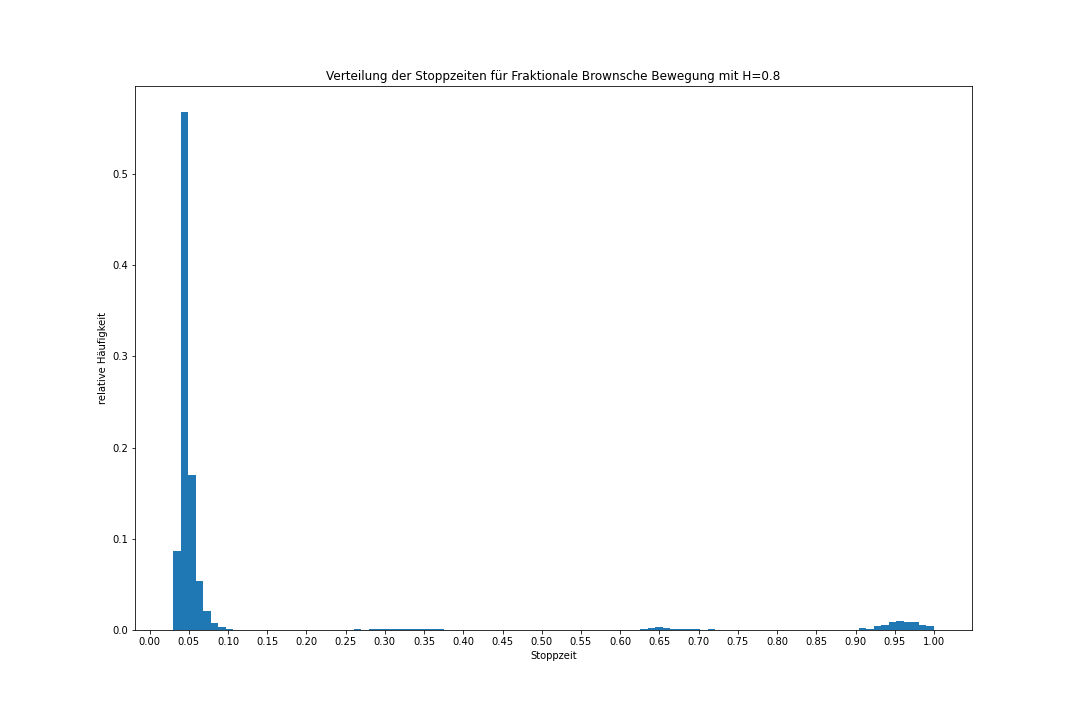
\includegraphics[width=.5\textwidth]{signatur/histogram_0_8.png}}
        \subfigure[Hybridmethode mit $H=0.8$]{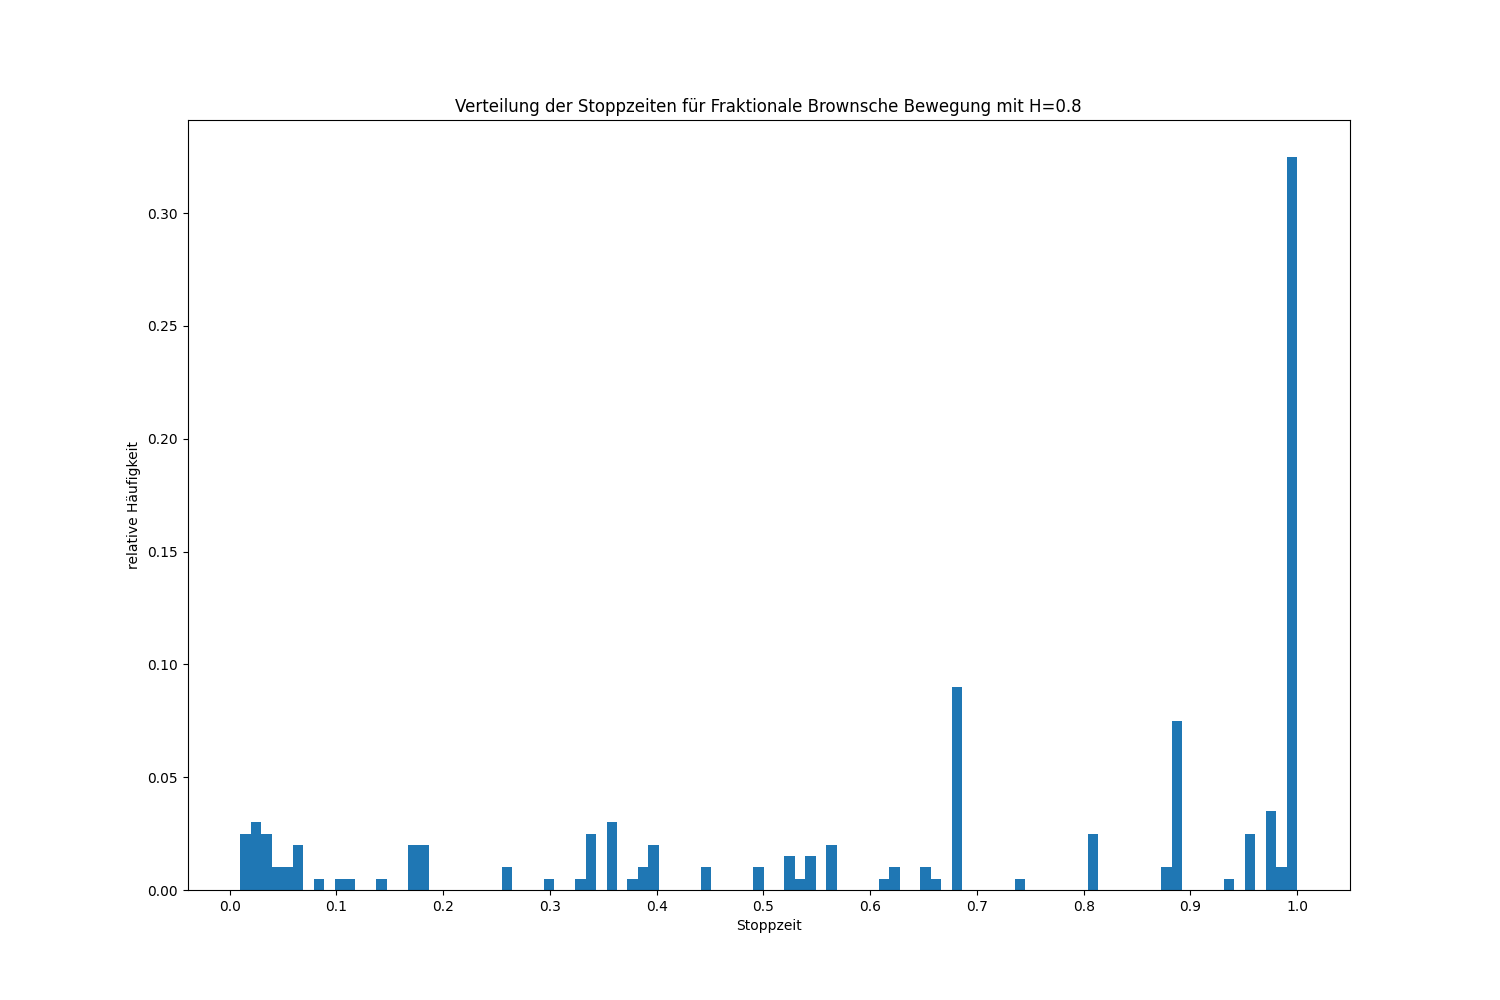
\includegraphics[width=.5\textwidth]{hybrid/histogram_0_8.png}}
      \end{figure}
      \begin{figure}[H]
        \subfigure[Signaturmethode mit $H=0.85$]{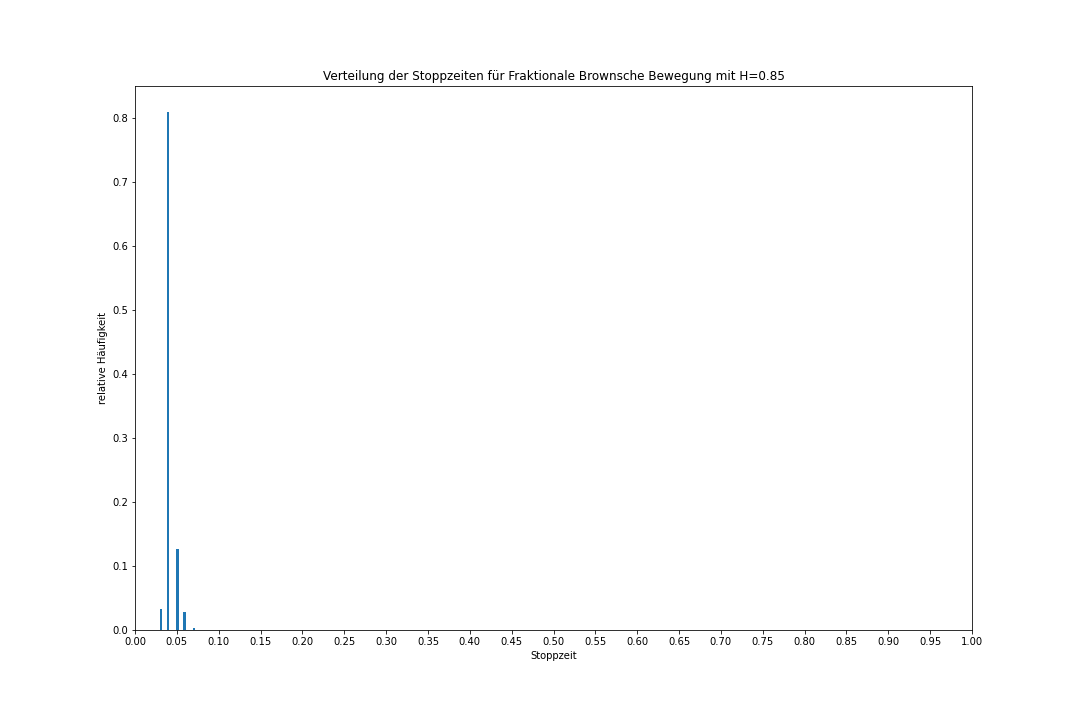
\includegraphics[width=.5\textwidth]{signatur/histogram_0_85.png}}
        \subfigure[Hybridmethode mit $H=0.85$]{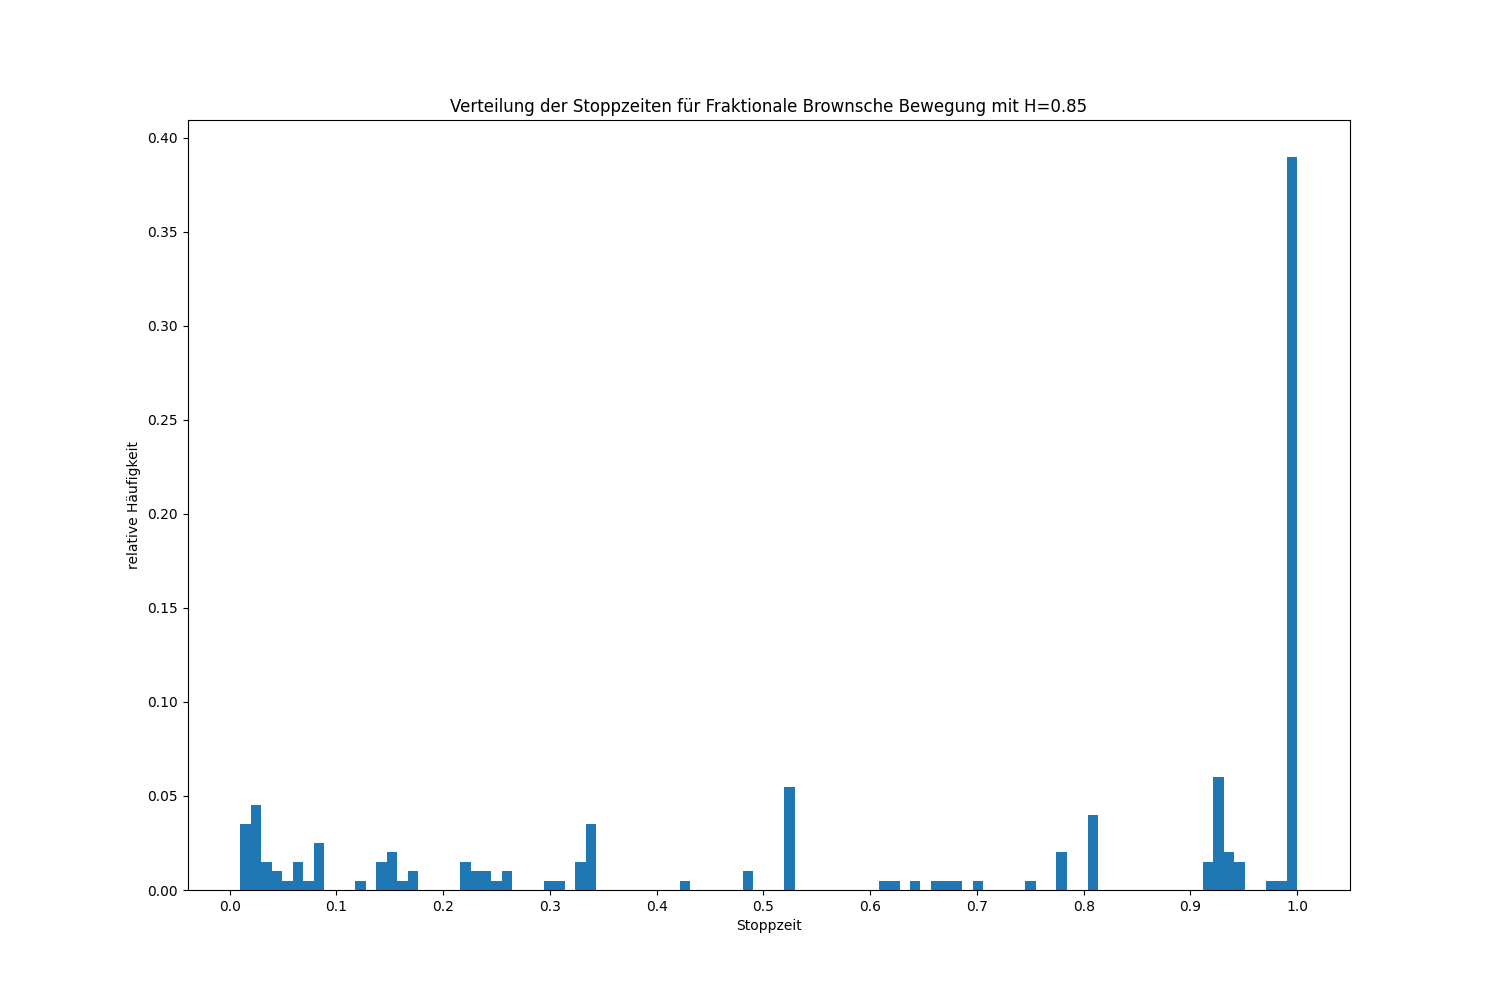
\includegraphics[width=.5\textwidth]{hybrid/histogram_0_85.png}}
        \subfigure[Signaturmethode mit $H=0.9$]{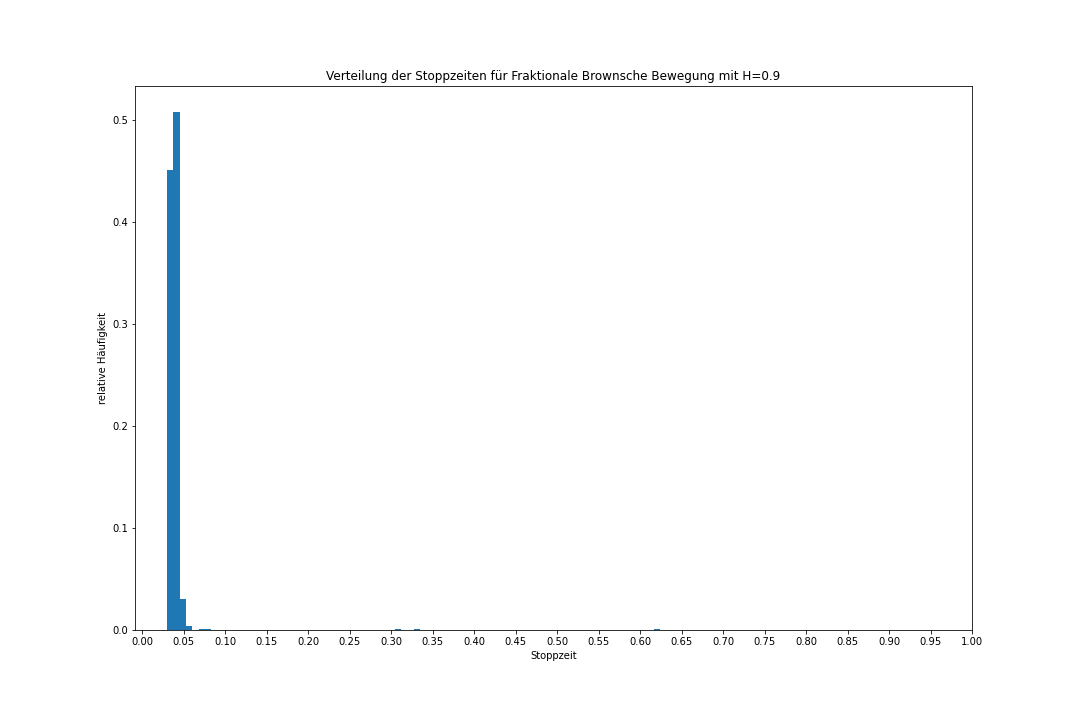
\includegraphics[width=.5\textwidth]{signatur/histogram_0_9.png}}
        \subfigure[Hybridmethode mit $H=0.9$]{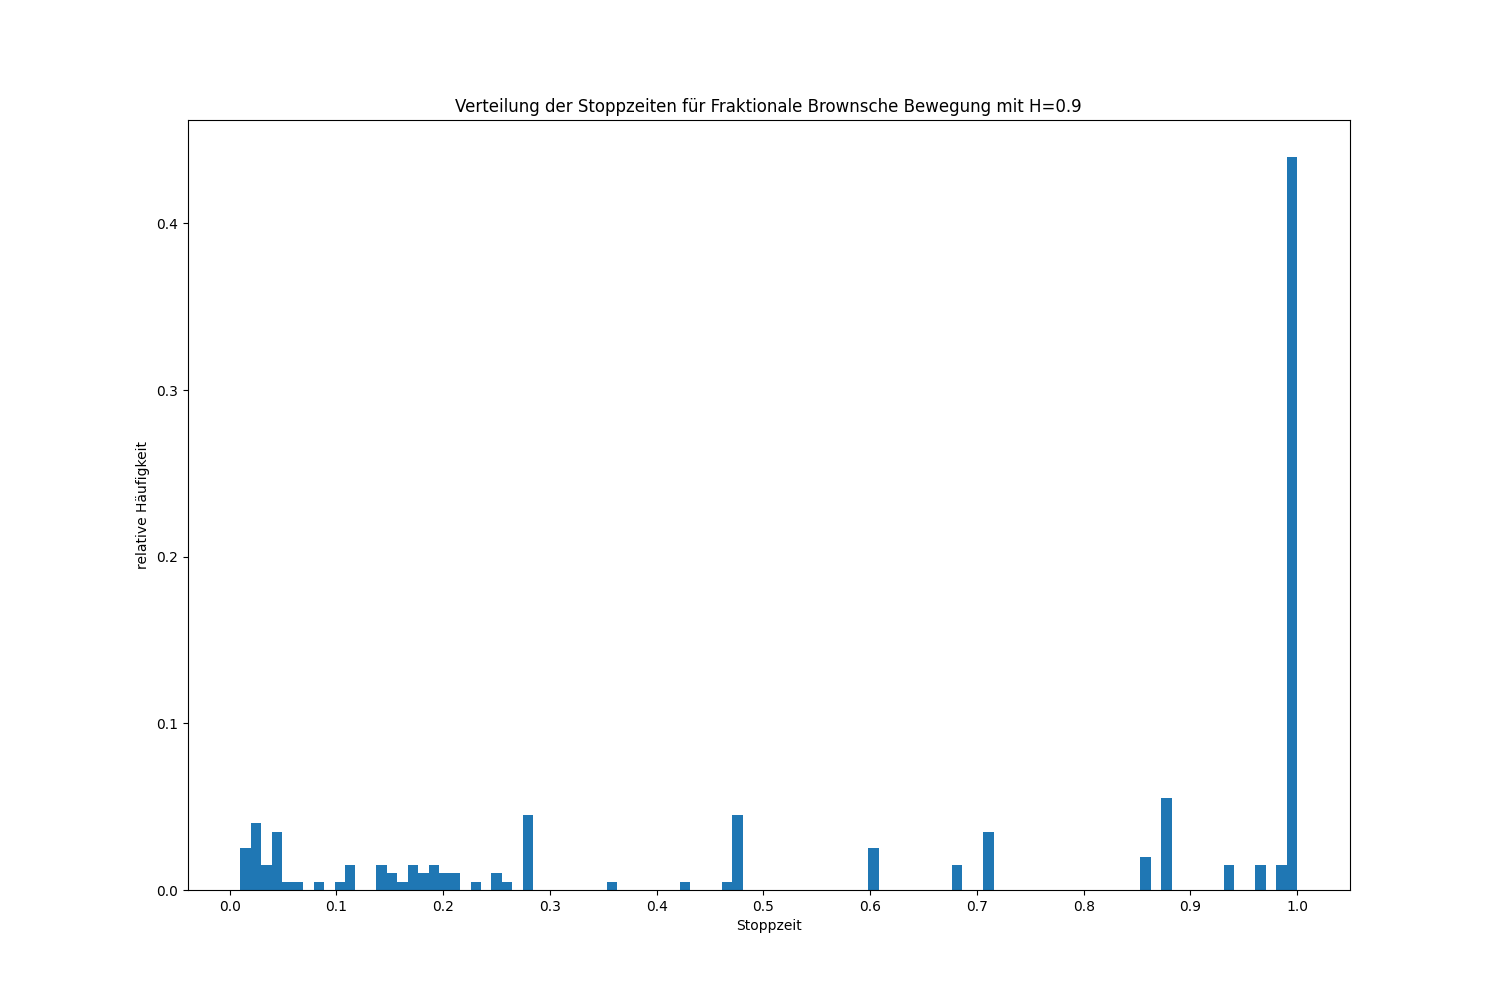
\includegraphics[width=.5\textwidth]{hybrid/histogram_0_9.png}}
        \subfigure[Signaturmethode mit $H=0.95$]{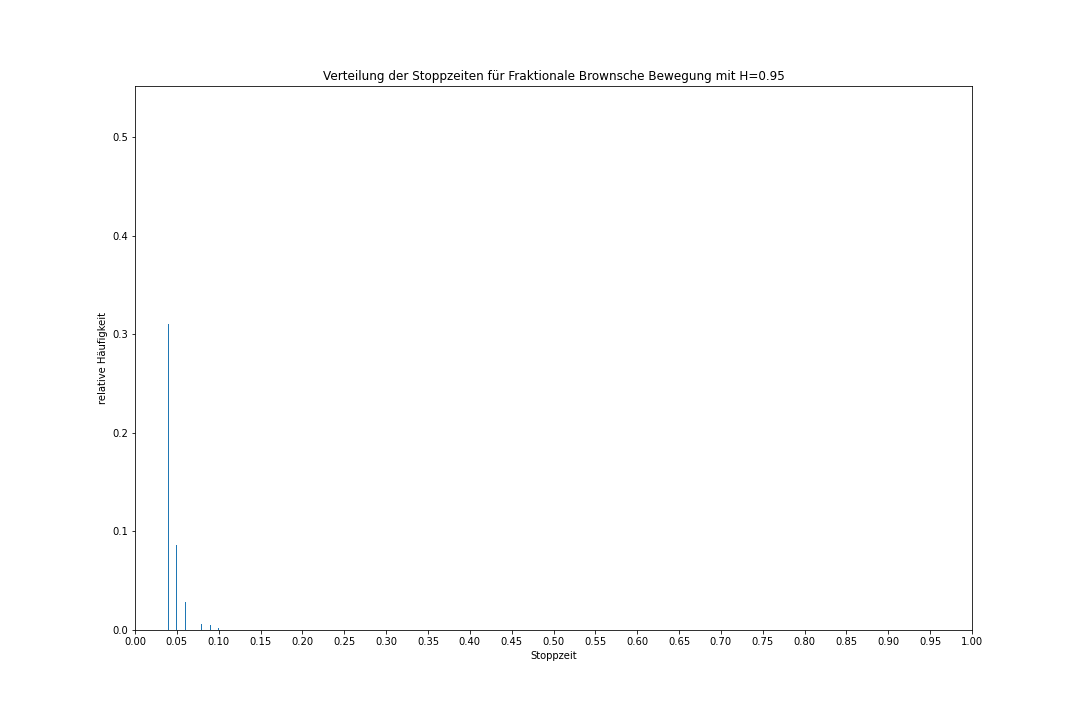
\includegraphics[width=.5\textwidth]{signatur/histogram_0_95.png}}
        \subfigure[Hybridmethode mit $H=0.95$]{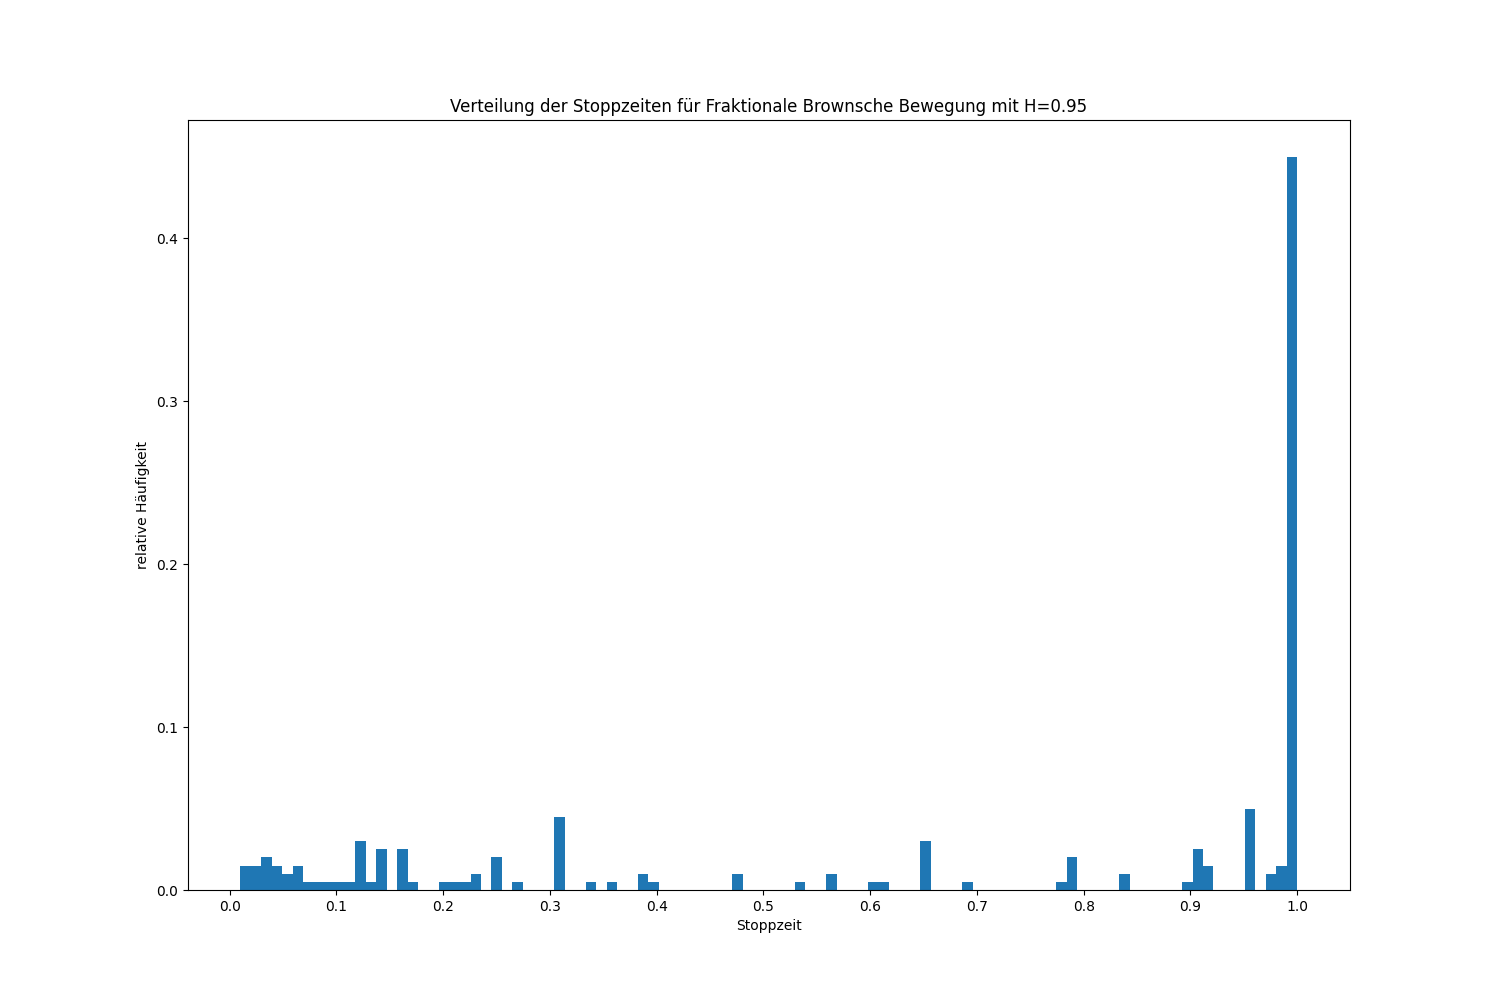
\includegraphics[width=.5\textwidth]{hybrid/histogram_0_95.png}}
      \end{figure}
      \newpage

\end{document}
